\documentclass[dvipsnames,letterpaper,12pt,titlepage,oneside,final]{memoir}

\usepackage{geometry}                % See geometry.pdf to learn the layout options. There are lots.
\geometry{letterpaper}                   % ... or a4paper or a5paper or ... 
%\geometry{landscape}                % Activate for for rotated page geometry
%\usepackage[parfill]{parskip}    % Activate to begin paragraphs with an empty line rather than an indent
\usepackage{epigraph}    %NEW
\usepackage{setspace} 
\usepackage{graphicx}
\usepackage{xcolor}
\usepackage{amssymb, amsmath}
\usepackage{epstopdf}

\DeclareGraphicsRule{.tif}{png}{.png}{`convert #1 `dirname #1`/`basename #1 .tif`.png}
\usepackage{tikz}
\usetikzlibrary{shadings, shadows, shapes, arrows, calc, positioning, shapes.geometric}

% \title{A note on the the theory of rent and urban economic development, August 20 2022}%\newline
% Financialization, Rent and Urban Economic Development
%Based on previous drafts , especially Financialization_of_the_Housing_Market .tex. June 27}

%\date{}                                           % Activate to display a given date or no date

\begin{document}
% \maketitle
\tableofcontents
t\chapter{Introduction}

Cities are a central feature of human society - Human beings are increasingly an urban species. Cities are one of the primary sources of technological development and increasing wealth. Behind these observations is a fundamental feature demonstrated in the recent literature on scaling laws: the productivity of cities increases super-linearly in population. Cities are the locus of a positive feedback loop: rising populations raises productivity, rising productivity attracts more people and resource.

Cities are where people live and work, where a great deal of production is concentrated, in addition to being where wealth is created and accumulated, cities are also where income is actually distributed. 

In Canada, there is a housing crisis. In the last few years, the need for affordable housing has come into focus as one of the most pressing issues facing Canadians. As more and more Canadians are finding housing unaffordable, the effects are being seen in everything from declining home ownership rates to an increasing number of Canadians unable to afford housing at all.

There has been extensive work on the drivers of the crisis, including supply shortages, stagnating incomes, and the finacialization of housing ownership.

There's been less work on the implications for productivity. The housing crisis raises the question of whether Canadian cities can continue to attract people and accumulate wealth for its residents and industries, whether in fact it can even sustain their growth.

This thesis presents a spatial model of the city that incorporates distributional issues and financialization and allows us to examine the productivity implications of the housing crisis. The model that incorporates the scaling of productivity in cities within a standard urban model. 
The urban model is based on those developed in geography, planning and urban economics. The organizing principle in  the spatial models of all three disciplines is an economic variable, land rent, which is the link to distribution, financialization and continuing productivity. *** (another sentence on why this is great)

The analysis makes clear that in addition to the recognized distributional consequences, the housing crisis has productivity impacts that should be considered in developing urban and housing policy. 


\subsection{OVERVIEW OF DOCUMENT}
\color{blue}

\textbf{In chapter XXX}  we link classical rent theory, neoclassical production theory, neoclassical growth theory, the scaling literature, and urban spatial models.
To show how our model is directly connected with this broad collection of linked theories, we use the Cobb-Douglas function, which is used across this entire range of literature 

After we develop the mathematical description of the relationship among these will discuss  in more detail, rent theory and our contribution, scaling laws, ......  and other issues in the literature that draw on parts of this model and 

???  apply to the specific situation we're in why rent theory is related to discussions of exploitation why it might lead the inefficiencies, whether or not this links with other important models in the literature.

\textbf{In chapter XXX} we  provide a description of finacialization and show it is a a form of rent-seeking in the housing market and ?? the potential consequences of fiancialization in the housing market. 



\textbf{In chapter XXX} we  describe an illustrative agent-based model of the urban system. Most of the analysis of urban systems has employed analytical models with roots that go back to von Thunen () and more recently Alonzo. These models are extremely useful, but necessarily abstract from the concrete  and variable individual behaviour and  the details  of dynamics that make real cities path-dependent. XXX (Dawn) have shown that agent-based models can reproduce the features of the analytical models, at least in simple cases. ABMs can be run multiple times to produce distributions of expected outocomes, which makes them valuable in planning exercises.  Our model is intended to be elaborated  for such use. 

After we develop the mathematical description of the relationship among these will discuss in more detail, various relevant applications, and issues in the literature that draw on parts of this model and apply to the specific situation we're in why rent theory is related to discussions of exploitation why it might lead the inefficiencies, whether or not this links with other important models in the literature.


\color{red}
Because we draw on a wide range of methods and literatures, we discuss the relevant literature and  nethodologies in the chapters where they apply 

\color{black}


Methodological questions: 

    - agent models (integrating theory more completely into agent models)
    
    - rent theory

Core model

    - static version
    
    - dynamic version

Simulations

Result---> hysterisis

policy

\subsubsection{OR (rougher):}

1. the core model and analysis - do a model of the endogenous dynamics of the model.

2. the resilience analysis -
but this is coupled with a larger system. we're interested in how it is coupled..

low interest rates have been key to financialization 
now they're going up?

we drive the system with signals to see how. and look at the external driving variables.

but what happens with changing interest rates? to explore we drive the system with external signal to explore how it is coupled with the larger economy and get an interesting resilience result, that it is actually a kind of ratchet pumping wealth out of communities on the upswing and on the downswing.

add interest, get a result which is hysteresis, which has policy implications
We get predictions about the implications of rising interest rates.

3.  policy analysis - finally we take a second step out to position the model within a larger dynamical system and do a systems analysis of the model and suggest policy implications. 

----------

% ?Ideally, an analysis of the current state of cities will incorporate supply, 
what do we want for the long introduction and background

\textbf{Ricardo concluded, significantly, that, ``It follows then, that the interest of the landlord is always opposed to the interest of every other class in the community.'' }


Our model has three stages: first, a production function, modeling how urban regions generate wealth,  second a spatial model of an urban housing market, and third, an analysis of distribution within that model 

In this section, we introduce the basic structure of the production side and connect it to the literature on urban scaling. The basic scaling result at the level of the city allows us to incorporate the effect of agglomeration in a standard  circular-city model in a simple way, avoiding the need to explicitly model labour markets and firms.\footnote{Explicitly modeling labour markets and firms is a natural way to specify the model more completely, but it would require introducing many ancillary assumptions and selecting among alternative models of agglomeration, when when we want to focus on distributional and growth-affecting features of the system.}

\begin{enumerate}
    \item to introduce  the productive nature of cities we basically assume the presence of scaling. Given  that the scaling literature gives us an estimate of the economies of scale in a production function this allows us to simplify the model and focus on the features of the urban system rather than on fully specifying a production system. In our model, the city  exhibits economies of scale with respect to population directly. 

     \item  productivity of the city to generates an economic value for land that gives rise to rents

    \item  the rental value of land structures the spatial structure of the city

    \item we exploit the rent model and transport costs to get  distributional consequences
\end{enumerate}

\color{red}
\chapter{Antecedents of modern Urban Rent theory}
In this chapter, we link classical rent theory, neoclassical, production theory, neoclassical, growth theory, the scaling literature,  and urban spatial models. 

We use the Cobb-Douglas function %, which is used to cross this entire range of literature 
to show how our  model is directly connected with this broad collection of linked theories. Our model connects to the results in this chapter at four points:



\section{Classical production and distribution theory}


 \subsection{Ricardo}



Modern neoclassical production theory can be seen as having one of its origins in  Classical economic theory going back to the Physiocrates. The physiocratic school of economics was the first to see labor as the sole source of value but, for the physiocrats, in the context of the prevalent European rural society of the time, only agricultural labor created a surplus. Ricardo's famous 1815 discussion of capital and  land rent \footnote{\href{http://la.utexas.edu/users/hcleaver/368/368RicardoOnCornLaws.html}{An Essay on the Influence of a low Price of Corn on the Profits of Stock}; shewing the Inexpediency of Restrictions on Importation: With Remarks on Mr Malthus' Two Last Publications: "An Inquiry into the Nature and Progress of Rent," and "The Grounds of an Opinion on the Policy of restricting the Importation of Foreign Corn" } 
provides the cannonical reference. He considers three-factor, three-class model with great precision but without the use of mathematics.   
In classical economics, land rent is a surplus value\footnote{``By rent I always mean the remuneration given to the landlord for the use of the original power of the land.'' David Ricardo corn laws note 7.}. 
and as Saunders pointed out in 1902, ``Of the concrete forms of income that have usually been classed as surplus, the rent of land was the earliest to be defined; and so prominent a position has been given to it that the terms " rent" and " surplus" have come to be used interchangeably.''\footnote{Rent in Modern Economic Theory: An Essay in Distribution Author(s): Alvin Saunders Johnson, Publications of the American Economic Association, Nov., 1902, 3rd Series, Vol. 3, No. 4 (Nov., 1902), pp. 1-129}. Ricardo and

The great social question that Ricardo addressed  was who gets the surplus. % The question was pressing because it appeared that landlords were capturing the surplus without contributing to production while many of those who worked that land were very poor. 
We begin with Ricardo and the classical economists because our focus is land rents, but in the context of an urban economy. According to Simon N. Patten, \footnote{Simon N. Patten,  The Quarterly Journal of Economics, volume 7, Issue 3, April 1893, Pages 322–352, https://doi.org/10.2307/1884006 }  Ricardo was ``the first writer to take the industrial phenomenon of city life and to create an economy based upon those characteristics.'' %Ricardo uses his model to explain the distribution of the product of the earth among the “three classes of the community” which is to say, to the owners of land, labour, and capital. 
In a passage that can be seen as a direct precursor to our analysis of urban land rent, Ricardo  wrote in his 1817 Principles of Political Economy, %

\begin{quotation}   
 “The produce of the earth - all that is derived from its surface by the united application of labour, machinery, and capital, is divided among three classes of the community; namely, the proprietor of the land, the owner of the stock or capital necessary for its cultivation, ad the labourers by whose industry it is cultivated. ...  But in different stages of society, the proportions of the whole produce of the earth which will be allotted to each of these classes, under the names of rent, profit, and wages, will be essentially different; ”  Chapter 1
\end{quotation}

Strikingly, Ricardo concluded\vootnote{An Essay on the Influence of a low Price of Corn} that, “It follows then, that the inter-
est of the landlord is always opposed to the interest of every other class in the community.” This is a view that Henry george would later pick up and it is one that we approach in our study, since the issue of urban rents is of great policy importance


\subsection{A more explicit treatment}
Ricardo expounded a theory of land rent, but he did not write down a formal production function as later neoclassical theorists would. In modern notation, Ricardo's model can be written


\begin{equation} 
Y=F(K,L,N).
\label{Eqn:Prod1}
\end{equation} 
where $K$ is capital, $L$ is labour and $N$  is the natural resource  land.\footnote{In principle any number of factors can be included.} 
Ricardo does not specify a functional form, but, like mathematical neoclassical economists, he does assume diminishing returns to all factors. The landlord  receives the surplus generated by the land and the rest of the value of production goes to labour and any capital employed in improving the land. 

The value of the land is the present discounted value of the surplus it generates

Most modern neoclassical treatments of production simplify by omitting land: 

\begin{equation} 
Y=F(K,L).
\label{Eqn:Prod1}
\end{equation} 

Leaving land out of the model makes sense for a variety of reasons. According to the Ricardian theory, rent is a surplus above cost. It does not, therefore enter into price. Land is a fixed factor for society as a whole that is not consumed in  the process of production.  Furthermore, neoclassical treatments of production  focus price determination and on the capitalist organization of production. 

% HOUSING RENT IN THE NATIONAL ACCOUNTS
%   Owner-occupied housing is included in Peersonal Consumption Expenditure because the National Income and Producgt Accounts (NIPAs) treat the owner-occupant as if it were a rental business, or in other words, a landlord renting to him or herself. That is, BEA imputes a value for the services of owner-occupied housing (space rent) based on the rents charged for similar tenant-occupied housing, and this value is included in GDP as part of personal consumption expenditures. This imputation is necessary in order for GDP to be invariant when housing units shift between tenant occupancy and owner occupancy.


%Ricardo  clearly understood and used the concept of diminishing marginal product. This shows in his use of the terms ``extensive margin'' and ``intensive margin'' to explain the income of the landowner. He focussed on the difference between the cost of production on a unit of land and the revenue generated. The landlord would rent out all the land which generated at least enough to pay all the costs. Anything in excess of the costs could be charged as land rent to a tenant farmer.



%Clearly in his model there are two basic productive factors, land and labour. The landlord  receives the surplus generated by the land and the rest of the value of production goes to labour. 
Recent urban models, on the other hand, tend to ignore the production process and consider the locational implications of land and transportation costs location of people. Wealth distribution is often ignored. 

\subsection{Marx}

Ricardo, agreeing with Malthus, essentially assumes that the wage is  just sufficient to reproduce the labouring class.\footnote{``In the natural advance of society, the wages of labour will have a tendency to fall, as far as they are regulated by supply and demand; for the supply of labourers will continue to increase at the same rate, while the demand for them will increase at a slower rate.''} He then explains the distribution of the fruits of labour on the land among the main classes of the economy.

 Marx shifted attention to a  manufacturing economy in which the owners contributed the machinery, buildings, and even working capital to fund the workers until the product can be sold. %This contribution must be accumulated from their profits in the preceding cycle of production,  and has to be reinvested once the revenues of the current round have come in and the bills have been paid. Marx actually describes a circuit of capital from its form as money to its form as physical capital. 
As in Ricardo, however, labour is in surplus and capital is scarce. As in Ricardo the scarce factor owned by a special class - now the capitalists, is able to appropriate the is able to capture the surplus value. Like Ricardo,  Marx saw the appropriation of surplus as without moral justification. 

Marx pointed to a new dynamic in capitalist systems - that productive capital is not fixed as land is, but  expands as surplus is reinvested. He famously suggested that the expansion will eventually outrun the expansion of demand and the rate of return will fall, leaving capitalists unwilling to invest and creating a crisis.


 
\subsection{Henry George} 
  Henry George, an influential American political economist,\footnote{Progress and Poverty: An Inquiry into the Cause of Industrial Depressions and of Increase of Want with Increase of Wealth: The Remedy (1879) book by social theorist and economist Henry George.}  returned to land rent with a new insight based on the emergence of the capitalist city: ``With the growth of population, land grows in value, and the men who work it must pay more for the privilege.'' For George the owners of urban land extract surplus in exactly the same way that owners of agricultural land in Ricardo's analysis. Where Marx saw  the extravagant productivity of capital  as the source of capitalist crises, George saw the extraction of wealth by land speculators as the mechanism that would bring on crises.
  
  Since land rent is not created by its owners, George argued that land rent should be seen as a social income - that it could be used to pay for all the needs of the community. The clearest statement of this view is found in Progress and Poverty: "We must make land common property." The same view was expressed by the Physiocrats who concluded  that ``ground rents'' should be the source of most or all taxes. They defined ground rent as that portion of all rent which is attributable only to the size and location of the parcel. George's analysis the `single tax' movement, which sought to shift all taxation to land  and resource rents.   
  
  In 1977, Joseph Stiglitz  showed, using a standard urban model, identified the conditions in which Henry George's "single tax" is  the only tax necessary to finance public expenditures.\footnote{Arnott, Richard J.; Joseph E. Stiglitz (November 1979). "Aggregate Land Rents, Expenditure on Public Goods, and Optimal City Size" (PDF). Quarterly Journal of Economics. 93 (4): 471–500. doi:10.2307/1884466. JSTOR 1884466. S2CID 53374401 }   The logic is fairly simple: if the public good increases productivity or the attractiveness of a city, attracting more people or businesses, land rents rise, and investment in the public good should proceed until the marginal cost of the public good is equal to the increase in land rent it brings. The result is now called the `Henry George theorem.'


The classical economists agreed that rents are unearned income. They did not emphasize, as George did, that land rents arise from labour's proximity to urban population and production.\footnote{To be fair, it was not lack of understanding, that the omission reveals, but rather lack of interest in explicitly examining urban land rent from residential or even industrial purposes.}% Ricardo von Thunen, Marx, Cantillon all grasped the notion of proximity to the market as part of the source land rent. The discussions seem to not gone farther than discussions of diffeerential and rents, however.  I just am not aware of them explicitly examining urban land rent for residential or even industrial purposes. 

%The need to be near a market or prodduction center is easily seen by considering a population at the carrying capacity of the land with individuals supporting themselves using purely local resources. There can be no land rent in this case. If a city rises that must be supplied from those still on the land, land close enough to the city will generate land rent. The value of the land is created by proximity to the city.



%  no separate and comprehensive data are provided on the amounts of land rents and subsoil rents charged and earned, because they are not officially regarded as part of value-added, and consequently are not included in the calculation of GDP (except for the value of productive lease contracts)     https://en.wikipedia.org/wiki/Differential_and_absolute_ground_rent#Rent_in_macro-economics    \href{https://en.wikipedia.org/wiki/Differential_and_absolute_ground_rent#Rent_in_macro-economics}{Wikipediat article on differential rent}



  \subsection{John Bates Clark and neoclassical distribution theory}
  Classical theories of distribution showed that ownership of a scarce and non-produced factor, land, was the  basis of rent extraction by the class of landowners. Profits were a bit puzzling in this context - Capital also earns its return from scarcity. Marshall pointed out, however, that scarcity profits (i.e., rent) would normally be competed away  as entrepreneurs entered the market in pursuit of those `excess' profits. He used the term `pseudo-rents' for these unearned but temporary incomes.\footnote{Alvin Saunders Johnson. Rent in Modern Economic Theory: An Essay in Distribution. AEA 3rd Series, Vol. 3, No. 4 (Nov., 1902), pp. 1-129 (129 pages)}

  
 John Bates Clark was one of the pioneers of marginalism and the neoclassical theory of  distribution.  The marginalist approach emphasized the rational decisions of economic agents in allocating their resources would lead them to allocate resources according to the value of the marginal product of he resource in production.  Initially a socialist like George, by 1986 he was praising the dynamical process of competition partly in opposition to the single tax movement George had initiated.  His (1891) ``Distribution as Determined by a Law of Rent,'' argued that, given  competition and homogeneous factors of production labor and capital, the division of the social product will be according to the productivity of the last (or marginal) physical input of units of labor and capital.\footnote{Responding to the "indictment that hangs over society" that it involves "exploiting labor," Clark wrote:

    It is the purpose of this work (his 1899 'Distribution of Wealth) to show that the distribution of the income of society is controlled by a natural law, and that this law, if it worked without friction, would give to every agent of production the amount of wealth which that agent creates. However wages may be adjusted by bargains freely made between individual men (i.e., without labor unions and other "market imperfections", the rates of pay that result from such transactions tend, it is here claimed, to equal that part of the product of industry which is traceable to the labor itself; and however interest (i.e., profit) may be adjusted by similarly free bargaining, it naturally tends to equal the fractional product that is separately traceable to capital.} 
 
Clark's analysis of income distribution does not contradict the classical view of rents, it simply displaces the analysis to the point where a competitive equilibrium prevails, and shifts attention away from the distribution of land rents. Rents are not earned by the marginal unit of land and  

\section{Neoclassical production theory}
The concept of a production function used by increasingly mathematical neoclassical economists and  rapidly developing statistical techniques  naturally led to attempts to identify the precise functional form that would describe the contributions of labour, capital and income to output.
 
Mathematician Charles Cobb and Economist Paul Douglas came up with a specific and very convenient functional form\footnote{Cobb, C. W.; Douglas, P. H. (1928). "A Theory of Production"  American Economic Review. 18 (Supplement): 139–165. JSTOR 1811556. Retrieved 26 September 2016. The function had apparently previously been used by Knut Wicksell, Philip Wicksteed, and L\'eon Walras.} that captured much of what economists were talking about. The function is just a generalized arithmetic mean:
 
 \[Y=AK^\alpha L^\beta\]
 where $A$ is a constant scale factor, commonly called `Total Factor Productivity'. 

%The Cobb Douglas function has several convenient features. One is that the sum of the coiefficents tells us the degree of returns to scale. If $\alpha+\beta = 1$, we have constant returns to scale,

%Another is that the coefficients of the factors, $\alpha$  and $\beta$ turn out to be the elasticities of output with respect to capital and labour respectively as well as the income share of the factor. These made it relatively easy for economists to combine national data on labour and capital stocks or income with output to test the model.

The Cobb–Douglas form was developed and almost immediately tested against statistical evidence in the USA by Cobb and Douglas between 1927–1947. It was  their widely circulated empirical work seems to have permanently associated this simple function with Cobb and Douglas for economists.

The Cobb-Douglas form captured  important regularities in the cross-sectional national data,\footnote{ A 2021 meta-analysis of 3186 estimates concluded that "the weight of evidence accumulated in the empirical literature emphatically rejects the Cobb-Douglas specification."Gechert, Havranek, Irsova, Kolcunova (2021), "Measuring capital-labor substitution: The importance of method choices and publication bias", Review of Economic Dynamics, doi:10.1016/j.red.2021.05.003, S2CID 236400765. More sophisticated models  such as the CES and translog functions have been developed  since.} 
but the estimates soon showed a systematic bias with time series. Essentially the value of the $A$ seemed to rise over time. Something that was not captured in the initial model  contributed to productivity over time: 
 \[Y=A(t)K^\alpha L^\beta\]

  \section{Neoclassical growth theories}  

 \subsection{The Solow-Swann growth model}
In 1956 Robert Solow\footnote{A Contribution to the Theory of Economic Growth,  Robert M. Solow, The Quarterly Journal of Economics, Vol. 70, No. 1 (Feb., 1956), pp. 65-94. Stable URL: http://www.jstor.org/stable/1884513} provided a possible explanation, opening the field for a further series of refinements in an enterprise that became known as ``growth theory.'' 

{\color{blue}  Both Solow and Denison were attempting to account for the main features of U.S. economic growth, not to provide a theory of economic development,  Denison's 1961 monograph, \textit{The Sources of Economic Growth in the United States}.  from R.E. Lucas, Jr., On the mechanics of economic development.}

Solow argued ``As a result of exogenous population growth the labor force increases at a constant relative rate n,'' so
  \[L(t)= L_0e^{nt}\] 
If we stick this into the production function 
 \begin{eqnarray}
 Y&=cK^\alpha (L_0e^{nt})^\beta\\
    &=c(e^{nt})^{\beta}K^\alpha L^\beta\\
  %  &=A(t)K^\alpha L^{1-\alpha} \label{Eq:Solow}
 \end{eqnarray}
we see that $A$ becomes
 \[A(t)=c(e^{nt})^\beta\]
The time-dependent term that allowed the model to track the data better. More than half  of the cross-country variation in income can be explained by per capita saving and population growth alone. However, the effects of saving and population growth on income are too large. To understand the relation between saving, population growth, and income, one must go beyond the textbook Solow model.t

%???       It is no surprise that adding a variable allowed the model to track the data better. More  interesting is that the appearance of term $1-\alpha}$ in the scale factor $A$ suggests a spillover effect of human capital on the productivity of other factors.\footnote{Breton, T. R. (2013). "Were Mankiw, Romer, and Weil Right? A Reconciliation of the Micro and Macro Effects of Schooling on Income" (PDF). Macroeconomic Dynamics. 17 (5): 1023–1054. doi:10.1017/S1365100511000824. hdl:10784/578. S2CID 154355849.}  

%The estimated model explained 78\% of variation in income across countries.
% the estimates of $\beta$ implied that\textbf{ human capital's external effects on national income are greater than its direct effect on workers' salaries.}%(\url{https://en.wikipedia.org/wiki/Solow\%E2\%80\%93Swan_model)}.  Theodore Breton provided an insight that reconciled the large effect of human capital from schooling in the Mankiw, Romer and Weil model with the smaller effect of schooling on workers' salaries. He demonstrated that the mathematical properties of the model include significant external effects between the factors of production, because human capital and physical capital are multiplicative factors of production.[20] The external effect of human capital on the productivity of physical capital is evident in the marginal product of physical capital:
%    \[ MPK={\frac {\partial Y}{\partial K}}=\frac {\alpha A^{1-\alpha }(H/L)^{\beta }}{(K/L)^{1-\alpha} }\]


Solow's 1956 paper stimulated a vast literature in the 1960s, exploring many variations on the original one-sector structure. % (per Lucas on mechanics) , See Burmeister and Dobell (1970) for an excellent introduction and survey. 
in these models the population growth rate determines the growth trend of the economy.

Robert E. Lucas observed  in 1988 that, ``It seems to be universally agreed that the model ... is not a theory of economic development.   \dots while it is not exactly wrong to describe these differences (in GDP  growth rates, ) by an exogenous, exponential term like A(t) neither is it useful to do so. We want a formalism that leads us to think about individual decisions to acquire knowledge, and about the consequences of these decisions for productivity.''\ footnote{Lucas,  Robert E. On the Mechanics of Economic Development. Journal of Monetary Economics 22, 1988 3-42}

\subsection{endogenous growth models}

Endogenous growth theories make the increase in total factor productivity depend on optimizing decisions about human capital investment, invention, and investment in technology improvement. Firms  actively search for innovations, and the ability to appropriate profits determines the resources devoted to innovative activity  %See (OECD, 1992, Crafts, 1996). Growth depends on the incentives to in-vest in improving technology.% 


Kenneth Arrow's 1962 paper\footnote{The Economic Implications of Learning by Doing, Kenneth J. Arrow, The Review of Economic Studies
Vol. 29, No. 3, 1962, pp. 155-173 }  is recognized as a forerunner of recent models of endogenous growth. It proposed `what he called `an endogenous theory of the changes in knowledge which underlie intertemporal and international shifts in production functions.'' Human capital, $H$ is acquired is acquired through learning by doing. 



In 1992, N. Gregory Mankiw, David Romer %(not to be confused with Paul M. Romer, mentioned above and below) 
and David N. Weil analyzed Solow’s Model in their paper “Contribution to the Empirics of Economic Growth” and  showed that %Solow correctly predicts the directions of saving and population growth, but not the orders of magnitude. Furthermore they pointed out that, 
if the model was augmented by the factor of human capital $H$, it would fit the data even better (Mankiw et al. 1992). The model became\footnote{Because they work with time series, all the quantities are dated. We omit the time marker for notational simplicity.}
\[Y=H^\beta K^\alpha (AL)^{1-\alpha-\beta\]
As a proxy for  $H$ the authors use the percentage of the working-age population in secondary school.  With Human capital included, the Solow model explains up to  78\% of the cross-country variation in income. 

Models of this sort have been described as employing only passive learning because the proxy for learning is not a decisions variable: it is still exogenous to the firm. Newer growth theories postulate that technology is endogenous because it relies on the decision to invest in research and development and diffusion


%\section{Rent}In economics, rent is a surplus value, i.e. the difference between the price at which an output from a resource can be sold and its respective extraction and production costs, including normal return (DFID, 2003; Luchsinger \& M\:uller, 2003; Sharp, 2003; Stoneham et al., 2005).

%More briefly, rent is a surplus value after all costs and normal returns have been accounted for. Normal costs include  payment of all the factors of production at their market rate.(Labour at the going wage, Capital at the interest rate, supplies at their normal price). 



%It is convenient in this model to use a Cobb-Douglas utility function that has the property that a fixed fraction of income is spent on housing.  We can start with the assumption that earnings are fixed for the lifetime at the one-period wage, $w$. Then total spending on housing is $\beta Y, \beta <1$ and $ Y=w$. Let the transportation cost for a specific location $l$ be $T(l)$. The  equilibrium price at that location will be $P(l)= \beta Y-T(l)$.

N. Gregory Mankiw, David Romer, and David Weil created a human capital augmented version of the Solow–Swan model that can explain the failure of international investment to flow to poor countries.

    \[Y(t)=(A(t)K(t)^\alpha H(t)^\beta L(t))^{1-\alpha -\beta} \]
    
    From the Solow example we can see that if all the time functions are exponential we end up with equation~\ref{Eq:Solow} again.
    
 

(((((   scale Bettancourt does this at the city level with N. he adds the empirical demonstration of the fun ctiohn. We  simply use the estimat to    

The model implicitly has a Solow-Swan style production model incorporating Jacobs-style labor-augmenting agglomeration economies (\textbf{\color{blue} maybe the discussion of agglomeration theories goes here? }) 



\color{black}

\color{green}
\subsection{Rent seeking}
  Rent-seeking is the act of growing one's existing wealth without creating new wealth by manipulating the social or political environment. Rent-seeking activities have negative effects on the rest of society. They result in reduced economic efficiency through misallocation of resources, reduced wealth creation, lost government revenue, heightened income inequality,
\color{black}
\chapter{Antecedents of modern Urban Rent theory}
In this chapter, we link classical rent theory, neoclassical production theory, neoclassical growth theory, the scaling literature, and urban spatial models. 

We use the Cobb-Douglas function %, which is used to cross this entire range of literature 
to illustrate each link and to show how our model is directly connected with this broad collection of linked theories. 

The Cobb-Douglas function is a production function, expressing the output produced, in terms of inputs such as labour and capital.

Maybe a high levels of summary of where the chapter will go?
Early theorists like Ricardo described something
can be thought of as describing a three-factor, three-class model with great precision but without the use of mathematics.   


and modern complexity theoriest have derived relations with urban scaling, which it turns out can be represented in the same form.
Part of what this does is shows how these different litteratures may be understood in terms of the production functions, with a common relation. 

%Our model connects to the results in this chapter at four points:



\section{Classical production and distribution theory}


 \subsection{Ricardo}

Modern neoclassical production theory can be seen as having one of its origins in classical economic theory. % going back to the Physiocrates. 

% The physiocratic school of economics was the first to see labor as the sole source of value but, for the physiocrats, in the context of the prevalent European rural society of the time, only agricultural labor created a surplus. % actually? % detail for it was ag economy This was the theory? also the french enginneers- detail for start of math/calc-..
%The canonical reference for only agricultural labour mattering? For the definition of rent?

%Ricardo's famous 1815 discussion of capital and  land rent \footnote{ %\href{http://la.utexas.edu/users/hcleaver/368/368RicardoOnCornLaws.html}{An Essay on the Influence of a low Price of Corn on the Profits of Stock}; 
%showing the Inexpediency of Restrictions on Importation: With Remarks on Mr Malthus' Two Last Publications: "An Inquiry into the Nature and Progress of Rent," and "The Grounds of an Opinion on the Policy of restricting the Importation of Foreign Corn"} provides the canonical reference. 
% We haven't introduced this model or what kind of thing it is.

In Ricardo's analysis and in classical economics in general, the income or landowners, land rent, is a surplus value\footnote{``By rent I always mean the remuneration given to the landlord for the use of the original power of the land.'' David Ricardo corn laws note 7.}. 
% rent was so central to their analysis it came to be used as this.
and as Saunders pointed out in 1902, ``Of the concrete forms of income that have usually been classed as surplus, the rent of land was the earliest to be defined; and so prominent a position has been given to it that the terms " rent" and " surplus" have come to be used interchangeably.''\footnote{Rent in Modern Economic Theory: An Essay in Distribution Author(s): Alvin Saunders Johnson, Publications of the American Economic Association, Nov., 1902, 3rd Series, Vol. 3, No. 4 (Nov., 1902), pp. 1-129}. 

The core social question that Ricardo addressed  was who gets the surplus. % The question was pressing because it appeared that landlords were capturing the surplus without contributing to production while many of those who worked that land were very poor. 
We begin with Ricardo and the classical economists because our focus is land rents, but in the context of an urban economy. According to Simon N. Patten, \footnote{Simon N. Patten,  The Quarterly Journal of Economics, volume 7, Issue 3, April 1893, Pages 322–352, https://doi.org/10.2307/1884006 }  Ricardo was ``the first writer to take the industrial phenomenon of city life and to create an economy based upon those characteristics.'' %Ricardo uses his model to explain the distribution of the product of the earth among the “three classes of the community” which is to say, to the owners of land, labour, and capital. 
In a passage that can be seen as a direct precursor to our analysis of urban land rent, Ricardo  wrote in his 1817 Principles of Political Economy, %

\begin{quotation}   
 “The produce of the earth - all that is derived from its surface by the united application of labour, machinery, and capital, is divided among three classes of the community; namely, the proprietor of the land, the owner of the stock or capital necessary for its cultivation, and the labourers by whose industry it is cultivated. ...  But in different stages of society, the proportions of the whole produce of the earth which will be allotted to each of these classes, under the names of rent, profit, and wages, will be essentially different; ”  Chapter 1
\end{quotation}

Land rent is easily illustrated. Imagine a carter who picks up vegetables at the farm gate and transports them into tow, where he sells them to a  storekeeper. He pays  the farmer at one end of the trip and is paid at the other. For simplicity. let's say all farmers have the same cost of production and the carters simply pay that amount at the farm gate and always is paid the merchant price in town. 

Clearly, the carter makes a `profit'  on his trip to the  farm nearest to town, but there is a farm so far out  that transport costs   eat up all the profit on the trip. That is as far as the carter will go. Ricardo termed this the `extensive margin'. 

 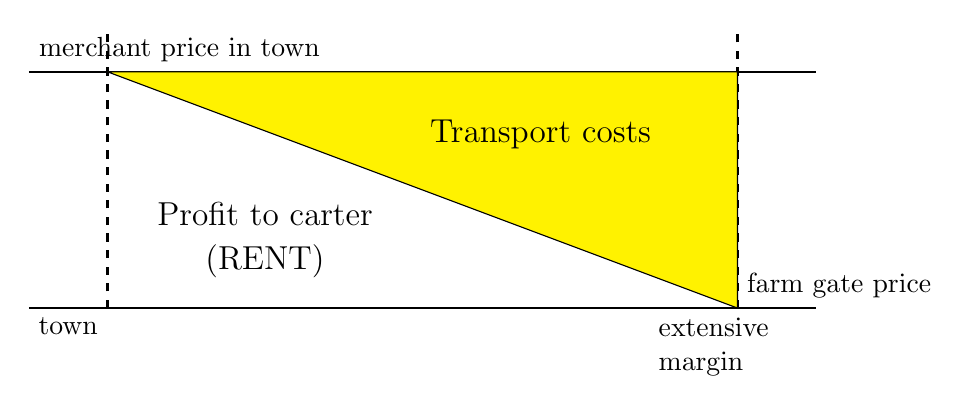
\begin{tikzpicture}[domain=0:2]
%\draw[thick,color=gray,step=.5cm, dashed] (-0.5,-.5) grid (3,3);
%\draw[line width=.01, green ] (0,0) -- (10,0) node[right  ] {Distance};
\node at (1,0) [below left] {town};
\draw[thick ] (0,3)node[above right] {merchant price in town} -- (10,3) ;
\draw[thick ] (0,0)  -- (10,0); 

draw[thick,color=red] (1.5,0) -- (1.5,1) node[below right] {Fixed cost} -- (1.5,1.5) --(10,3.25)node[above left] {total cost};
\draw[thick, dashed ] (1,0) -- (1,3.5) ;
\draw[thick, dashed ] (9,0)node[below,text width=2cm] {extensive margin} -- (9,3.5) ;
%\draw[ultra thick, blue,<-> ] (3,1.8) -- (3,2.5)node[left] {annual rent at a} -- (3,3) ; 
\draw[fill=yellow] (1,3) --(9,3)--(9,0) --cycle;
\node at (9,0)[above right] {farm gate price};
\node  at (6.5,2.2){\large Transport costs};
\node  at (3.,1.2){\large Profit to carter};
\node  at (3.,.6){\large (RENT)};
\end{tikzpicture}   

In the figure, total transport costs are shown as the yellow area. The area below the yellow triangle is profit for  the carter.\footnote{Compare the figure to one developed to illustrate Alonzo's urban model:


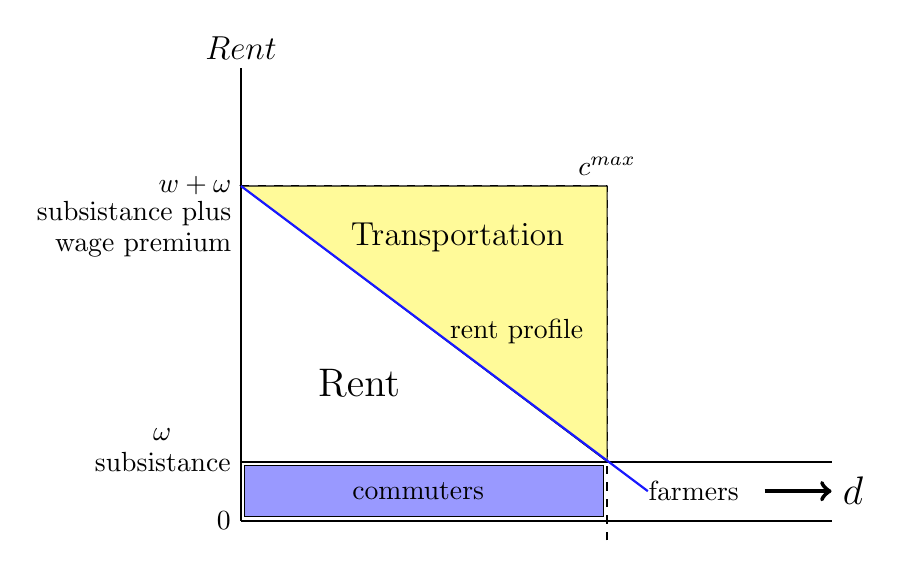
\begin{tikzpicture}[scale=.5]
\def\bndmax{5}        
\def\bndmin{0.2}
\def \n {10}  % height of y axis
\def \d {15}  % length  of x axis
\def \t {.75}  %  cost of transportation per unit x
\def \th {1}   %
\def \w {7}    %  wage premium
\def \om{1.5}%  omega =rural wage Zero for urban population
\def \azero{2}
\def \aprime {-.0}	
\tikzset{func/.style={thick,color=blue!90}}	

\draw [thick] (0,-\om) --(\d,-\om);  			% Zero for rural population
\draw [thick] (0,-\om)node[left]{$0$} --(0,\n);	% Y axis
\node at (0,\n+0.5){\large$Rent$};

\draw [thick] (0,0)node[left]{subsistance}--(\d,0);
\node a t(-2,.7) {$\omega$};
\node[left] at (0,\w){$w+\omega$};
\node[left] at (0,\w-.7){subsistance plus};
\node[left] at (0,\w-1.5){wage premium};	
\draw [dashed, thick](9.3,-2)-- (9.3,\w)node[above]{$c^{max}$};
\draw [dashed, thick](0,\w)-- (9.3,\w);
% solid color for commuters
\draw[fill=blue!40] (0.1,-0.1) rectangle (9.2,-\om+.1);
\draw[fill=yellow!40] (9.30,7.) -- (0,7)--(9.30,0.)--cycle;% Rent \w-.2
\draw[func,domain=0:\w/\t+1] plot [samples=200] (\x,{\w-\t*\x});
\node at (5.5,5.7){\large Transportation};
\node at (7,3.3){rent profile};		%Rent Profile	
\node at (3.,2){\Large Rent}; 		%Rent 
\node at (4.5,-\om/2){commuters};
\node at (11.5,-\om/2){farmers};
\draw [ ultra thick, ->](13.3,-\om/2)--(15, -\om/2)node [right] {\Large $d$};
 
 \end{tikzpicture}


} Together these areas represent the ``produce of the earth'', but only the lower triangle is net income\footnote{ Termed the `\textit{produit net}' by the Physiocrats}.   In modern supply and demand analysis it would be recognized as `producer surplus'.

Now consider Ricardo's case: the land owner delivers the grain to market and receives the merchant price. The profit now accrues to the landowner, and we call it land rent. For Ricardo, it was obvious that the land-owning class captured the land rent.\footnote{In the modern economy, agricultural land rents may be captured by corporations,  either by owning the land or by controlling the supply chain.}  Landlord income is a locational land rent that exists  because of the land's proximity to the market. 

Notice how the land rent declines with distance from the town,\footnote{It also declines as we move onto less fertile land.} At the extensive margin the land rent falls to zero. Even fertile land beyond the extensive margin will not be farmed because the product cannot be transported to market at a profit.\footnote{This simple example assumes that the land is uniformly productive and that there is only one product that can be marketed. Johann Heinrich von Th\"unen, in The Isolated state (Der isolierte Staat (1826)), provide a more complex analysis based on the same principles.} Transportation costs and the price of produce in town determine the size of the  rent triangle and therefore the amount of rent captured by the land-owning class.\footnote{The debate about the  `Corn Laws" that Ricardo  was engaged in was about whether Britain would allow wheat form Canada and Australia to enter, reducing the price of wheat and therefore reducing the income and influence of the land-owning class.} 


%\subsection{A more explicit treatment}
Ricardo expounded a theory of land rent, but he did not write down a formal production function as later neoclassical theorists would. In modern notation, Ricardo's model can be written


\begin{equation} 
Y=F(K,L,N).
\label{Eqn:Prod1}
\end{equation} 
where $K$ is capital, $L$ is labour and $N$  is the natural resource  land.\footnote{In principle any number of factors can be included.} 
Ricardo does not specify a functional form, but, like mathematical neoclassical economists, he does assume diminishing returns to all factors. The landlord  receives the surplus generated by the land and the rest of the value of production goes to labour and to any capital employed in improving the land. 

The value of the land is the present discounted value of the surplus it generates.

Most modern neoclassical treatments of production simplify by omitting land: 

\begin{equation} 
Y=F(K,L).
\label{Eqn:Prod1}
\end{equation} 

Leaving land out of the model makes sense for a variety of reasons. According to the Ricardian theory, rent is a surplus above cost. It does not, therefore enter into price. Land is a fixed factor for society as a whole that is not consumed in  the process of production.  Furthermore, neoclassical treatments of production focus price determination based on the cost of the last unit used, the marginal  unit of input, while rents are generated on all of the inframarginal units, those units used earlier, which are more productive. The marginal unit of land generates no rents. In neoclassical analysis, the rents disappeared from view for this reason. This difference is at the heart of the distinction between classical and neoclassical economic theory. 

%John B. Davis. Ricardo's Theory of Profit and the Third Edition of the \textit{Principles}. Journal of the History of Economic Thought, 15, Spring 1993. °1993 by the History of Economic Society.
%``Questions arise, however, when one turns to exchange between a sector paying rent and one not.'' The Principles tells us that as cultivation is extended and exchange increases, profits fall while rents increase. 

Leaving land out, however, creates a problem in  the neoclassical growth theories we will examine below. Under the assumption of perfectly competitive goods and factors markets as well as marginal productivity pricing of capital and labor, neoclassical growth requires technical change to be generated outside the model because there are no resources left to innovate if both factors of production are paid their marginal product.\footnote{This follows from Euler’s theorem: if, for a given level of technology $\bar A$ output Y is produced according to a \textbf{constant returns to scale} and twice continuously differentiable function of capital and labor $F(K, L, \bar A)$, Euler’s theorem implies that $F_K K + F_L L=Y$, where $F_i$ is the marginal product of factor $i$. Payments to  capital and labor take up the entire national product and no resources are left to finance the production of technology-improving innovations. are paid their marginal product.} 
If, however, land is reintroduced, as it must be in an urban model, there must be rents and there is therefore as surplus available for innovation.
\footnote{An alternative and common approach is to assume imperfect competition, which may be based on increasing returns to scale, in which case firms with market power may achieve a surplus. ``Although seldom modeled outside the monopolistic competition framework, market incompleteness and imperfect competition are central to the new growth theories'' (Gilles Duranton, Growth and imperfect competition on factor markets: Increasing returns and distribution, European Economic Review, 44-2, 2000, 255-280), Similarly, Sjak Smulders and Theo van de Klundert conclude that ``Growth is higher in a more concentrated market provided that market power of firms is not too high,'' (Imperfect competition, concentration and growth with firm-specific R \& D, European Economic Review, 39-1, 1995,139-160).}
%I have not followed this track down to give you references.

% ALSO Imperfect Competition and Total Factor Productivity Growth  AZZEDDINE M. AZZAM, ELENA LOPEZ and RIGOBERTO A. LOPEZ. Journal of Productivity Analysis. Vol. 22, No. 3 (November, 2004), pp. 173-184 (12 pages)

%Sjak Smulders and Theo van de Klundert.Imperfect competition, concentration and growth with firm-specific R & D European Economic Review. Volume 39, Issue 1, January 1995, Pages 139-160
% Duranton, Gilles (1997) Essays on growth: imperfect competition, labour supply and local public goods. PhD thesis, London School of Economics and Political Science.  http://etheses.lse.ac.uk/1471/1/U105715.pdf

%Alberto Bucci.  R&D, Imperfect Competition and Growth with Human Capital Accumulation, 2003. Scottish Journal of Political Economy. https://doi.org/10.1111/1467-9485.5004004. This paper studies the long-run consequences of imperfect competition on growth and the sectoral distribution of skills within an R&D-based growth model with human capital accumulation. We find that steady-state growth is driven only by incentives to accumulate skills. In the model imperfect competition has a positive growth effect, while influencing the allocation of human capital to the different economic activities employing this factor input. Contrary to general wisdom, the share of resources invested in R&D turns out not to be monotonically increasing in the product market power and its correlation with the equilibrium output growth rate is not unambiguous.

%NOTE URBAN COMPETITION PROVIDES INCENTIVES TO UPGRADE SKILLS!!!


% Both the Solow (1956) growth model and its Ramsey–Cass–Koopmans counterpart featuring an endogenous saving rate (Ramsey, 1928; Cass, 1965; Koopmans, 1965) see technical change as purely exogenous. In fact, under the assumption of perfectly competitive goods and factors markets as well as marginal productivity pricing of capital and labor, neoclassical growth requires technical change to be generated outside the model because there are no resources left to innovate if both factors of production. 

%  This follows from Euler’s theorem: if, for a given level of technology $\bar A$ output Y is produced according to a constant returns to scale and twice continuously differentiable function of capital and labor $F(K, L, \bar A)$, Euler’s theorem implies that $F_K K + F_L L=Y$, where $F_i$ is the marginal product of factor $i$. Hence, remunerating capital and labor takes up the entire national product, and no resources are left to finance the production of technology-improving innovations. Accordingly, the growth rate of technology will $\frac{\dot{A}}{A}=g_A$ is necessarily exogenous. %Focusing on balanced growth and 
% assuming that technical progress is labor augmenting (Uzawa, 1961), we can rewrite the production function as $F(K, AL$), where $AL$ is a measure of labor in efficiency units, or effective workers. Let k = K/(AL). Then, output per effective worker is y =Y/(AL)=f (k). Population grows at the constant rate n > 0 and, as we will assume throughout the whole paper, capital does not depreciate. The steady state of the Solow model solves

% $\frac{f(k_{ss}}{k_{ss}} = \frac{n+g_A}{s}kss s$

% Journal of Economic Surveys (2017) Vol. 31, No. 5, pp. 1272–1303 \c ECONOMIC THEORIES 1275


Classical rent re-appears in neoclassical theory as `economic rent' (``a money payment made for a factor of production that is over and above the minimum payment to keep it in its present use,'')  as quasi-or pseudo-rents (non-equilibrium rents that will be competed away in a competitive equilibrium according to Marshall.\footnote{see Lewis Cecil Gray Rent Under the Assumption of Exhaustibility, Quarterly Journal of Economics, May, 1914, Vol. 28, No. 3 (May, 1914), pp. 466-489}),  as consumer  and producer surplus in supply and demand analysis,  as rent profiles or Pseudo-rent curves in urban theory, as a major concern on resource economics, and the theory of rent-seeking. Economic rent is a surplus insofar as its payment is not necessary to ensure a supply of a particular factor of production. 


% HOUSING RENT IN THE NATIONAL ACCOUNTS
%   Owner-occupied housing is included in Peersonal Consumption Expenditure because the National Income and Producgt Accounts (NIPAs) treat the owner-occupant as if it were a rental business, or in other words, a landlord renting to him or herself. That is, BEA imputes a value for the services of owner-occupied housing (space rent) based on the rents charged for similar tenant-occupied housing, and this value is included in GDP as part of personal consumption expenditures. This imputation is necessary in order for GDP to be invariant when housing units shift between tenant occupancy and owner occupancy.


%Ricardo  clearly understood and used the concept of diminishing marginal product. This shows in his use of the terms ``extensive margin'' and ``intensive margin'' to explain the income of the landowner. He focussed on the difference between the cost of production on a unit of land and the revenue generated. The landlord would rent out all the land which generated at least enough to pay all the costs. Anything in excess of the costs could be charged as land rent to a tenant farmer.



%Clearly in his model there are two basic productive factors, land and labour. The landlord  receives the surplus generated by the land and the rest of the value of production goes to labour. 
Recent urban models, on the other hand, tend to ignore the production process and consider the locational implications of land and transportation costs location of people. Wealth distribution is often ignored. 

\subsection{Marx}

%Ricardo, agreeing with Malthus, essentially assumes that the wage is  just sufficient to reproduce the labouring class.\footnote{``In the natural advance of society, the wages of labour will have a tendency to fall, as far as they are regulated by supply and demand; for the supply of labourers will continue to increase at the same rate, while the demand for them will increase at a slower rate.''} He then explains the distribution of the fruits of labour on the land among the main classes of the economy.

 Marx shifted attention to the manufacturing economy in which the owners contributed the machinery, buildings, and even working capital to fund the workers until the product can be sold. %This contribution must be accumulated from their profits in the preceding cycle of production,  and has to be reinvested once the revenues of the current round have come in and the bills have been paid. Marx actually describes a circuit of capital from its form as money to its form as physical capital. 
As in Ricardo, however, labour is in surplus and capital is scarce. As in Ricardo the scarce factor owned by a special class - now the capitalists, is able to appropriate the is able to capture the surplus value. %Like Ricardo,  Marx saw the appropriation of surplus as without moral justification. 

Marx pointed to a new dynamic in capitalist systems - that productive capital is not fixed as land is, but  expands as surplus is reinvested. He famously suggested that the expansion will eventually outrun the expansion of demand and the rate of return will fall, leaving capitalists unwilling to invest and creating a crisis. 


 
\subsection{Henry George} 
  Henry George, an influential American political economist,\footnote{Progress and Poverty: An Inquiry into the Cause of Industrial Depressions and of Increase of Want with Increase of Wealth: The Remedy (1879) book by social theorist and economist Henry George.}  returned to land rent with a new insight based on the emergence of the capitalist city: ``With the growth of population, land grows in value, and the men who work it must pay more for the privilege.'' For George the owners of urban land extract surplus in exactly the same way that owners of agricultural land in Ricardo's analysis. Where Marx saw  the extravagant productivity of capital  as the source of capitalist crises, George saw the extraction of wealth by land speculators as the mechanism that would bring on crises.
  
  Since land rent is not created by its owners, George argued that land rent should be seen as a social income - that it could be used to pay for all the needs of the community. The clearest statement of this view is found in Progress and Poverty: "We must make land common property." The same view was expressed by the Physiocrats who concluded  that ``ground rents'' should be the source of most or all taxes. They defined ground rent as that portion of all rent which is attributable only to the size and location of the parcel. George's analysis the `single tax' movement, which sought to shift all taxation to land  and resource rents.   
  
  In 1977, Joseph Stiglitz  showed, using a standard urban model, identified the conditions in which Henry George's "single tax" is  the only tax necessary to finance public expenditures.\footnote{Arnott, Richard J.; Joseph E. Stiglitz (November 1979). "Aggregate Land Rents, Expenditure on Public Goods, and Optimal City Size" (PDF). Quarterly Journal of Economics. 93 (4): 471–500. doi:10.2307/1884466. JSTOR 1884466. S2CID 53374401 }   The logic is fairly simple: if the public good increases productivity or the attractiveness of a city, attracting more people or businesses, land rents rise, and investment in the public good should proceed until the marginal cost of the public good is equal to the increase in land rent it brings. The result is now called the `Henry George theorem.'


The classical economists agreed that rents are unearned income. They did not emphasize, as George did, that land rents arise from labour's proximity to urban population and production.\footnote{To be fair, it was not lack of understanding, that the omission reveals, but rather lack of interest in explicitly examining urban land rent from residential or even industrial purposes.}% Ricardo von Thunen, Marx, Cantillon all grasped the notion of proximity to the market as part of the source land rent. The discussions seem to not gone farther than discussions of diffeerential and rents, however.  I just am not aware of them explicitly examining urban land rent for residential or even industrial purposes. 

%The need to be near a market or prodduction center is easily seen by considering a population at the carrying capacity of the land with individuals supporting themselves using purely local resources. There can be no land rent in this case. If a city rises that must be supplied from those still on the land, land close enough to the city will generate land rent. The value of the land is created by proximity to the city.



%  no separate and comprehensive data are provided on the amounts of land rents and subsoil rents charged and earned, because they are not officially regarded as part of value-added, and consequently are not included in the calculation of GDP (except for the value of productive lease contracts)     https://en.wikipedia.org/wiki/Differential_and_absolute_ground_rent#Rent_in_macro-economics    \href{https://en.wikipedia.org/wiki/Differential_and_absolute_ground_rent#Rent_in_macro-economics}{Wikipediat article on differential rent}



  \subsection{John Bates Clark and neoclassical distribution theory}
  Classical theories of distribution showed that ownership of a scarce and non-produced factor, land, was the  basis of rent extraction by the class of landowners. Profits were a bit puzzling in this context - Capital also earns its return from scarcity. Marshall pointed out, however, that scarcity profits (i.e., rent) would normally be competed away  as entrepreneurs entered the market in pursuit of those `excess' profits. He used the term `pseudo-rents' for these unearned but temporary incomes.\footnote{Alvin Saunders Johnson. Rent in Modern Economic Theory: An Essay in Distribution. AEA 3rd Series, Vol. 3, No. 4 (Nov., 1902), pp. 1-129 (129 pages)}

  
 John Bates Clark was one of the pioneers of marginalism and the neoclassical theory of  distribution.  The marginalist approach emphasized the rational decisions of economic agents in allocating their resources would lead them to allocate resources according to the value of the marginal product of the resource in production.  Initially a socialist like George, by 1986 he was praising the dynamical process of competition partly in opposition to the single tax movement George had initiated.  His (1891) ``Distribution as Determined by a Law of Rent,'' argued that, given  competition and homogeneous factors of production labor and capital, the division of the social product will be according to the productivity of the last (or marginal) physical input of units of labor and capital.\footnote{Responding to the "indictment that hangs over society" that it involves "exploiting labor," Clark wrote:

    It is the purpose of this work (his 1899 'Distribution of Wealth) to show that the distribution of the income of society is controlled by a natural law, and that this law, if it worked without friction, would give to every agent of production the amount of wealth which that agent creates. However wages may be adjusted by bargains freely made between individual men (i.e., without labor unions and other "market imperfections", the rates of pay that result from such transactions tend, it is here claimed, to equal that part of the product of industry which is traceable to the labor itself; and however interest (i.e., profit) may be adjusted by similarly free bargaining, it naturally tends to equal the fractional product that is separately traceable to capital.} 
 
Clark's analysis of income distribution does not contradict the classical view of rents, it simply displaces the analysis to the point where a competitive equilibrium prevails, and shifts attention away from the distribution of land rents. Rents are not earned by the marginal unit of land and  

\section{Neoclassical production theory}
The concept of a production function used by increasingly mathematical neoclassical economists and  rapidly developing statistical techniques  naturally led to attempts to identify the precise functional form that would describe the contributions of labour, capital, and income to output.
 
Mathematician Charles Cobb and Economist Paul Douglas came up with a specific and very convenient functional form\footnote{Cobb, C. W.; Douglas, P. H. (1928). "A Theory of Production"  American Economic Review. 18 (Supplement): 139–165. JSTOR 1811556. Retrieved 26 September 2016. The function had apparently previously been used by Knut Wicksell, Philip Wicksteed, and L\'eon Walras.} that captured much of what economists were talking about. The function is just a generalized arithmetic mean:
 
 \[Y=AK^\alpha L^\beta\]
 where $A$ is a constant scale factor, commonly called `Total Factor Productivity. This function becomes the workhorse of neoclassical growth theory in the second half  of the 20th century. Our urban model is a direct heir of those developments.

%The Cobb Douglas function has several convenient features. One is that the sum of the coefficents tells us the degree of returns to scale. If $\alpha+\beta = 1$, we have constant returns to scale,

%Another is that the coefficients of the factors, $\alpha$  and $\beta$ turn out to be the elasticities of output with respect to capital and labour respectively as well as the income share of the factor. These made it relatively easy for economists to combine national data on labour and capital stocks or income with output to test the model.

The Cobb–Douglas form was developed and almost immediately tested against statistical evidence in the USA by Cobb and Douglas between 1927–1947. It was  their widely circulated empirical work seems to have permanently associated this simple function with Cobb and Douglas for economists.

The Cobb-Douglas form captured  important regularities in the cross-sectional national data,\footnote{ A 2021 meta-analysis of 3186 estimates concluded that "the weight of evidence accumulated in the empirical literature emphatically rejects the Cobb-Douglas specification."Gechert, Havranek, Irsova, Kolcunova (2021), "Measuring capital-labor substitution: The importance of method choices and publication bias", Review of Economic Dynamics, doi:10.1016/j.red.2021.05.003, S2CID 236400765. More sophisticated models  such as the CES and translog functions have been developed  since.} 
but the estimates soon showed a systematic bias with time series. Essentially the value of the $A$ seemed to rise over time. Something that was not captured in the initial model  contributed to productivity over time: 
 \[Y=A(t)K^\alpha L^\beta\]

  \section{Neoclassical growth theories}  

 \subsection{The Solow-Swann growth model}
In 1956 Robert Solow\footnote{A Contribution to the Theory of Economic Growth,  Robert M. Solow, The Quarterly Journal of Economics, Vol. 70, No. 1 (Feb., 1956), pp. 65-94. Stable URL: http://www.jstor.org/stable/1884513} provided a possible explanation, opening the field for a further series of refinements in an enterprise that became known as ``growth theory.''
\footnote{Solow and his contemporary, Edward F. Denison in his 1961 monograph, \textit{The Sources of Economic Growth in the United States}, were attempting to account for the main features of U.S. economic growth, not to provide a theory of economic development.}%   R.E. Lucas, Jr., On the mechanics of economic development.}

Solow argued ``As a result of exogenous population growth the labor force increases at a constant relative rate n,'' so
  \[L(t)= L_0e^{nt}\] 
If we insert this term into the production function 
 \begin{eqnarray}
 Y&=cK^\alpha (L_0e^{nt})^\beta\\
    &=c(e^{nt})^{\beta}K^\alpha L^\beta\\
  %  &=A(t)K^\alpha L^{1-\alpha} \label{Eq:Solow}
 \end{eqnarray}
we see that $A$ becomes
 \[A(t)=c(e^{nt})^\beta\]
and we have a version of the time-dependent term needed to  allow the model to track the data better. More than half  of the cross-country variation in income can be explained by per capita saving and population growth alone.



%???       It is no surprise that adding a variable allowed the model to track the data better. More  interesting is that the appearance of term $1-\alpha}$ in the scale factor $A$ suggests a spillover effect of human capital on the productivity of other factors.\footnote{Breton, T. R. (2013). "Were Mankiw, Romer, and Weil Right? A Reconciliation of the Micro and Macro Effects of Schooling on Income" (PDF). Macroeconomic Dynamics. 17 (5): 1023–1054. doi:10.1017/S1365100511000824. hdl:10784/578. S2CID 154355849.}  

%The estimated model explained 78\% of the variation in income across countries.
% the estimates of $\beta$ implied that\textbf{ human capital's external effects on national income are greater than its direct effect on workers' salaries.}%(\url{https://en.wikipedia.org/wiki/Solow\%E2\%80\%93Swan_model)}.  Theodore Breton provided an insight that reconciled the large effect of human capital from schooling in the Mankiw, Romer, and Weil model with the smaller effect of schooling on workers' salaries. He demonstrated that the mathematical properties of the model include significant external effects between the factors of production because human capital and physical capital are multiplicative factors of production.[20] The external effect of human capital on the productivity of physical capital is evident in the marginal product of physical capital:
%    \[ MPK={\frac {\partial Y}{\partial K}}=\frac {\alpha A^{1-\alpha }(H/L)^{\beta }}{(K/L)^{1-\alpha} }\]


Solow's 1956 paper stimulated a vast literature in the 1960s, exploring many variations on the original one-sector structure. % (per Lucas on mechanics), See Burmeister and Dobell (1970) for an excellent introduction and survey. 
In these models, saving and population growth rates determine the growth trend of the economy. An important  contribution of the neoclassical framework stems from its ability to quantify the effects of various influences on growth. The estimated influences of saving and population growth with the Solow model appear too large, however.%Ludcas on the mechanics of ec dev
\footnote{In 1992, N. Gregory Mankiw, David Romer %(not to be confused with Paul M. Romer, mentioned above and below) 
and David N. Weil analyzed Solow’s Model in their paper “Contribution to the Empirics of Economic Growth” and  showed that %Solow correctly predicts the directions of saving and population growth, but not the orders of magnitude. Furthermore they pointed out that, 
if the model was augmented by including human capital $H$, it would fit the data even better.   (Mankiw et al. 1992). Their equation was, in our notation   \[Y=A(t)K^\alpha H^\gamma L^\beta\label{Eq:Mankiw}\] They assume $\alpha+\gamma<1$ which implies decreasing returns to all capital.}

To understand the relation between saving, population growth, and income, it was necessary to go beyond the textbook Solow model, which assumed  diminishing returns to capital and labor separately and constant returns to both factors jointly,


 MISSED Mankiw et al equation 
 % The  model became\footnote{Because they work with time series, all the quantities are dated. We omit the time marker for notational simplicity.}

In 1988, Robert E. Lucas would observe that ``It seems to be universally agreed that the model ... is not a theory of economic development.   \dots while it is not exactly wrong to describe these differences (in GDP  growth rates) by an exogenous, exponential term like A(t) neither is it useful to do so. We want a formalism that leads us to think about individual decisions to acquire knowledge, and about the consequences of these decisions for productivity.''\footnote{Lucas,  Robert E. On the Mechanics of Economic Development. Journal of Monetary Economics 22, 1988 3-42} 

% NOTE for  K   
%If we replace the labor-capital technology of the Solow model with a land-labor technology of the same form, and treat labor as the mobile factor and land as the immobile, we obtain a model that predicts exactly the immigration flows that occurred and for exactly the reason - factor price differentials - that motivated these historical flows



One of the predictions of the neoclassical growth model, even  when the concept of capital includes human capital, is that without  continuing improvements in technology, per capita income growth eventually ceases on the equilibrium path. 
By treating technological change as exogenous, neoclassical growth theory could not focus on the fundamental forces which determine long-run growth of nations. Theorists got around the problem to some extent by assuming that technological progress occurs in an exogenous manner. 

The models that followed, starting with Arrow's  1962 model of `learning by doing', introduce human capital and learning in a variety of ways. This is a central insight. Human capital may enter  as a stock that accumulates in the firm or the sector (Arrow (1962), Levhari (1966), and Sheshinski (1967b)) (proxied by aggregate prior capital investment.)
%(Levhari-Sheshinski)as  the experience of workers, the number of units previously produced, 
or the amount of innovation in other firms and sectors. % ( King and Robson )


Identifying  plausible ways that human capital might affect development was relatively easy. Measurement of human capital presents great practical difficulties. To extract the implications of a particular path, it was also necessary to construct a tractable model, analyze its dynamic properties, and find proxy data to test the initial hypothesis.   A series of papers did exactly that.

Kenneth Arrow (1962) gave a dynamic interpretation to increasing returns by emphasizing 'Learning by Doing'. This was an early attempt to render technological progress endogenous in growth models by making the productivity of a given firm an increasing function of cumulative aggregate investment for the industry. Productivity rises with cumulative firm output.


 It is important to note that these models all open the possibility that governments can  promote growth through investment in education, research, technology transfer, and incentives for firms.

\subsection{Endogenous (neoclassical) Growth Models}
A new wave of research on economic growth was stimulated by Romer (1986) and Lucas (1988). In their models, returns to scale are external to single economic agents and internal to a sector or larger parts of the economy. We apply the same insight to urban models to incorporate the growth-enhancing effect of agglomeration. 

%Basically, two branches have developed, pioneered by Romer (1990) and Lucas (1988). CHECK THESE SOURCES

Paul Romer's 1986  model\footnote{ based on his 1983 thesis} describes `learning by investment'. In this model, the increase in total factor productivity depends on firms’ learning, or investment in knowledge accumulation through research, rather than output. He models the incentives for the production of knowledge explicitly. The production function  can be written

\[Y = A(R^T)R^\gamma  K^\alpha L^\beta) \]
Where $R(\equiv R_i)$ is the research effort of the specific firm, and $R^T=\sum_iR_i$ is the total research in the industry,  $R$ is a choice variable for the firm, which is to say, it decides how much to invest in research. 

A notable feature of this model is the spillover effect on all other firms of the firm's investment through the Total Factor Productivity term,  $A(R^T)$. \textbf{This is the logic of our own model of agglomeration effects in the city.}



In 1988 Lucas also argued that technical progress is not exogenous, but endogenous. He proposed a model that is very close technically to the similar models of Arrow (1962), Uzawa (1965)and Romer (1986). Following our notation, 
\[ Y = A(H^e) K^\alpha (HeL)^\beta \] 
where $H^e$ is the economy's average level of skill (human capital).  Improvements in skill in any firm  increase overall productivity.  $HeL$  can be understood as the `effective' labour force of the firm. It is a product of $L$, size of the workforce. $H$, is the skill level of the firm's workers, and $e$, is the fraction of work time spent working. $1-e$ is the fraction of worker time  spent in training. The  special feature is that $e$ is a choice variable for the firm.\footnote{It could as easily be a choice variable for workers in the aggregate model.} More time training increase $H$ but reduces $e$, so the firm faces a tradeoff.


The difference between Romer and Lucas style theories is that endogenous growth in the theory of Romer is caused by accumulating technology (or knowledge), while in Lucas it is through training (accumulating human capital)\footnote{Although it is not of direct concern for our work, it is useful to recognize that much of the emphasis in these models is on finding the conditions that can explain the observed long term  and growth over and above that driven by exogenous population or technology growth. }

%THIS NEXT PARAGRAPH A SIMPLE COPY. FIND SOURCE

Again we see the  internal effects of human capital, where the individual worker undergoing training becomes more productive, and an external or `spillover' effect which increases the productivity of the economy. 
The evidence supports the existence of significant learning spillovers in a variety of industries. Using survey data, Mansfield (1985) found that information about new processes and products in ten industries surveyed had widely diffused within a year. Spillovers have also been found in econometric studies: Irwin and Klenow (1994) find them in semiconductors; Thornton and Thompson (2001) in wartime shipbuilding; Lieberman (1989) in chemicals; Foster and Rosenzweig (1995) in the adoption of high-yielding seed varieties; and Conley and Udry (2007) in the adoption of best practices by Ghanaian pineapple farmers. 

\textbf{ NOTE for Kirsten:  Neoclassical  growth theory predicts that growth rates of different countries with same rates of saving and population growth and with access to the same technology will converge. In  endogenous growth theory there is no force leading to the convergence of growth rates of different countries with closed economies. If the logic extends to urban systems as we believe it does, growth rates of cities will also diverge.}

\subsection{Neoclassical Production Theory and the City}
%\href{https://www.yourarticlelibrary.com/economics/new-theory-of-growth-of-economic-development/38329}{New Theory of Growth of Economic Development}Supriya Guru

In all of these models, the unit of analysis is the nation,  or the firm. Lucas has suggested,\footnote{Journal of Monetary Economics 22 (1988) 3-42.  ON THE MECHANICS OF ECONOMIC DEVELOPMENT*
Robert E. LUCAS, Jr., University of Chicago, Chicago, 1L 60637, USA}
however, that `` a national economy is a completely arbitrary unit to consider.'' and that ``we know from ordinary experience that there are group interactions that are central to individual productivity and that involve groups larger than the immediate family and smaller than the human race as a whole.''  


As a result, ``following very closely the lead of Jane Jacobs, whose remarkable book The Economy of Cities (1969)'', Lucas goes on to suggest `` that the 'force' we need to postulate account for the central role of cities in economic life is of exactly the same character as the 'external human capital' I have postulated as a force to account for certain features of aggregative development.''  He concludes that if this is so, ``\textbf{\dots land rents should provide an indirect measure of this force (emphasis  ours)}, in much the same way that schooling-induced earnings differentials provide a measure of the productive effects of internal human capital. ''

This insight, which parallels ours, has not been adequately explored, in our view.  Allowing Lucas to expand on his observation, 


\begin{quotation}
    Her emphasis on the role of cities in economic growth stems from the observation that a city, economically, is like the nucleus of an atom: If we postulate only the usual list of economic forces, cities should fly apart. \textbf{The theory of production contains nothing to hold a city together.} (empahsis ours) A city is simply a collection of factors of production - capital, people, and land - and land is always far cheaper outside cities than inside. Why don't capital and people move outside, combining themselves with cheaper land and thereby increasing profits? Of course, people like to live near shopping and shops need to be located near their customers, but circular considerations of this kind explain only shopping centers, not cities. Cities are centered on wholesale trade and primary producers, and a theory that accounts for their existence has to explain why these producers are apparently choosing high rather than low-cost modes of operation.
\end{quotation}

This observation provides a natural link to the scaling literature on cities.


\section{Cities and the Scaling Literature}
Neoclassical production theory does not address the spatial structure of the economy. Why are there cities? What drives the historic transition from land-based agricultural society to a much denser urban society? 

In The Economy of Cities (1969) Jane Jacobs argued that when people come together in cities they make each other more productive. This is in essence, a theory of urban agglomeration that could be written
\begin{equation}\label{eq:LtoN}
Y = A(t) K(t)^\alpha L^\beta 
\end{equation}
where $L$ stands for the size of the urban labour force. Since urban labour force and population are closely correlated, the familiar model is  observationally equivalent to
\begin{equation}\label{eq:N2}
Y = A(t)N^{\alpha+\beta}
\end{equation}
\footnote{ To see why, let  $cN$ be labour employed by capital in firms, where $N$ represents the urban population and  assume a constant capital-labor ratio $1/d$. Replace $K$ with $dcN$
\[Y = A(t) (dcN)^\alpha (cN)^\beta) \]
But  $dc^\alpha$ and $c^\beta$  are simply  multiplicative constants that can be incorporated into the scale factor $A$, so  the function becomes 
\[Y = A(d, c,\alpha, \beta, t)N^{\alpha+\beta}\]
}

A model of a national economy that uses the number of urban dwellers would track as well using the number employed. As countries develop, cities account for an ever-increasing share of  national populations and an ever-increasing share of national income.  This is  even more likely when we recall that the principle insights coming out of neoclassical growth theory point to human capital and education as the mystery factor in growth and cities are where the most skilled workers concentrate and where the strongest educational institutions tend to be. The mysterious contribution to growth pursued in the previous sections might  actually be a consequence of urbanization.

We have conventional diminishing returns to scale  if we impose the standard neoclassical assumption, 
$\alpha +\beta <1 $.\footnote{
The required condition is that 
$Y(\delta K,\delta L< \delta Y(K,L)$. 
In the function that we use to illustrate the models, 
$Y(\delta K,\delta L)= \delta^{\alpha +\beta}Y < Y(K,L)$.} 
That leaves us with a question: what do we need for Equation~\ref{eq:N1} to represent Jacobs' observation?  

The answer lies in making the synergies that Jacobs point to explicit: we require $N$ to generate a spillover effect similar to those  identified in neoclassical growth theory. There are three obvious generic ways to introduce such a term: $N$ can augment $A$, $K$, or $L$, 

NEEDS ALIGNMENT
  
\[Y = A*N^\gamma K^\alpha N^\beta= AK^\alpha N^{\beta+\gamma}\]
\[Y = A (N^\gamma* K)^\alpha  N^\beta= AK^\alpha N^{\beta+\gamma^\alpha}\]
\[Y = A K^\alpha (N^\gamma* N)^\beta= AK^\alpha N^{\beta+\gamma}\]

Each of these yields a form of
\[Y = AN^\psi\]
where $\psi> \alpha +\beta$ and may be greater than one. 
The question now is whether we can find estimates of $\psi$.

The evidence we need comes from another field. Complex systems theory is concerned with identifying and characterizing common design elements that are observed across diverse natural, technological and social complex systems. It focuses on general principles  identified in complex systems across many fields such as biology, physiology, ecology, stock markets, multi-user online  networks, data systems, human settlements.and urban systems.

Scaling analysis is a tool developed in complex systems science to investigate how extensive properties of the system vary with a system's size.  or scale.  In urban science, there are now many studies of  the relationships between urban population size and  features like urban economic output,  area, growth, traffic congestion costs, and even social  indicators like crime and homicide rates. Our particular interest is in studies linking city population  and  economic output. 

The model used is familiar. Omitting subscripts for time, $t$ and city, $i$, \footnote{Bettancourt (2021) writes the model \[Y_i = Y_0(t)N_i(t)^\beta e^{\xi(t)}\]. }
\[Y = Y_0e^{n(t)}N^\beta\]
where $Y_0$ is an initial value. Notice that this looks exactly like the form that we saw in the 
Solow-Swan model with the transform from $K^\alpha L^\beta$ to $N$.  The interpretation is different because the model is used to estimate the parameter $\beta$ and $e^{n(t)}$ is described  as an error term of the form commonly used in estimating multiplicative time-series models. As a result estimates of $\beta$  can be used as estimates  of $\psi$.

\vspace{1cm}
\textbf{\Large COPY BOTTOM FIVE ROWS OF TABLE ON BETTANCOURT PAGE 67}  


\vspace{2cm}
The empirical scale factor is a feature of  a static urban system, but, as we have seen it is essentially a growth model. If the population rises, output must rise more than proportionately, but if the population responds to the share of output, the population should then rise. This is a 

Much of growth theory was concerned with identifying the dynamics of such systems and in particular with the implications for the growth of incomes. The growth models, however, were not spatial models, and therefore abstracted from land rents And distribution. They have nothing to say about the distribution of city product and the effect that distribution might have on growth.\footnote{Early models employ a macroeconomic savings function which usually has a fixed savings rate, with savings being reinvested in productive capital. } 

\vspace{2cm}

\section{Equilibrium city size  in terms of scale factor} 
At this point we can briefly describe how the discussion of this chapter relates to our overall modelling. There are four basic equations in the model. The first two link output and the wage to population. 

\subsubsection{population and output}
Equation one, following Bettencourt (p65) says that  urban productivity is proportional to population via a scale factor: 
\[Y\propto N^{\beta}\]  
\footnote{ In contemporary US cities productivity increases by about 11\% with each doubling of their population.  Urban Scaling and the Production Function for Cities Lobo J, Bettencourt LMA, Strumsky D, West GB (2013) PLOS ONE 8(3): e58407. https://doi.org/10.1371/journal.pone.0058407 },
and has both theoretical and empirical support. 

% \begin{tabular}{ll}
% $Y$ is &Aggregate urban output, or GDP \\
% %$\alpha$ & agricultural wage\\
% $G$ is&a `prefactor', possibly time dependent, an initial population\\
%  $N$ is& city population\\
% $ \beta$  is& scale factor, the elasticity of output with respect to city population .\\
% \end{tabular}\vspace{.5cm}

This is illustrated below for $\beta=1.13$.

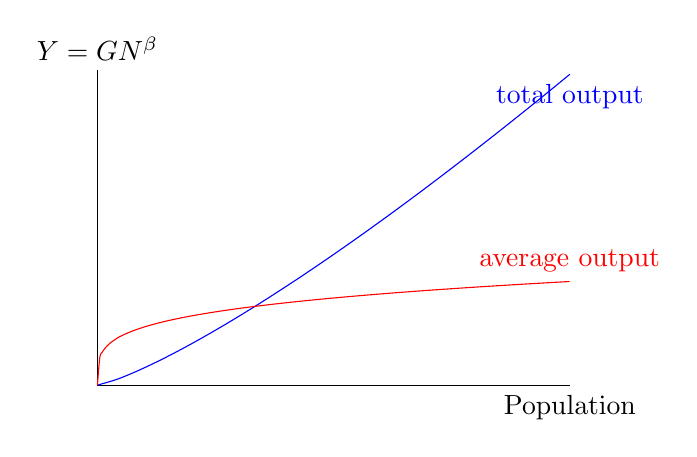
\begin{tikzpicture}
  \draw (0,4)node[above]{$Y= GN^{\beta}$}--(0,0) --(6,0)node[below]{Population};
   \draw[scale=1, domain=0:6, smooth, variable=\x, blue] plot ({\x}, {(\x/2)^1.25})node[below]{total output };% divide by 2 to get it on the plot
   %\draw (0,1)node[left]{$\alpha$}--(6,3.5)node[left]{$\alpha +\rho P$};
  \draw[scale=1, samples=200,domain=0:6, smooth, variable=\x, red] plot ({\x}, {(\x/2)^.25})node[above]{average output};% THis is the wage plot
       %   \draw[red] plot[samples=200, domain=-0:6] function {(\x/2)^.25};%node[above]{wage};
  %  \node [left] at (0,2){$w=\rho P$};
     % \draw [dashed](0,3)node[left]{$Y_i$}--(6,3);
 \end{tikzpicture}\vspace{.5cm}
 
 This figure illustrates a worry for me - the \textbf{average income} - {a proxy for the wage?) rises with $N$ but not more rapidly than transportation costs.
 
\subsubsection{Output and wage}
We need a combination of classical and neoclassical distribution theory.

City output is divided among the classes of society. Neoclassical theory suggests wages are allocated according to marginal product and classical theory suggests rents according to the pattern of ownership.

Eqaution one, in effect determines a wage, (Given the observed values for the scaling coefficients for total wages and labor, $bW < 1.15$ and $bL < 1$, )  although there are many possible distributional specifications and many possible labour market and firm structures. Bettencourt provides two  estimates,  1.11 and 1.35, for the scale factor for urban personal income in the Brazil and South Africa respectively.\footnote{A more recent  study supports the Bettancourt results for Chiin Wu W, Zhao H, Tan Q, Gao P. An Urban Scaling Estimation Method in a Heterogeneity Variance Perspective. Entropy (Basel). 2019 Mar 28;21(4):337. doi: 10.3390/e21040337. PMID: 33267051; PMCID: PMC7514821.} 

\subsubsection{Wage and city size}
The third determines the extent of the city. This comes form the Alonzo model discussed in chapter XXXXA.  A simple case is the circular city with uniform transportation cost, $t$. \[r^*= \frac{w}{t}\]% A more complex model might have density depend on location, for example, in the continous circular cityt\,
If transportation costs vary by  distance we might have something like this constraint on extent\[w=\int_0^{d*} t(d)dt.\]

This approach imposes an equilibrium condition on the model. It is unnecessary working with a citation of known extent and density. The analytic approach is easily extended to variable transportation cost, although at the expense of additional computational complexity.

\subsubsection{City extent and population}
Equation  four  closes the model by linking the extent of the city to the population. A simple case is the circular city with uniform population $d$, where $d$ is density per unit area and $r^*$ is the radius of the city: \[P=d\pi r^{*2}\] 
More generally, density might vary with for example, the distance $r$ from the centre of the city:
\[P=\pi \int_{0}^{r*}d(r)\,dr\] In a computational model a table of densities would provide the link.


\subsubsection{challenges}
maybe discuss some of the modeling challenges - division of income, lags, ???

\color{black}


\vspace{2cm}


\color{green}
 The growth of many cities was initially fueled by agricultural rents and resource exports. The industrial revolutions transformed many of these consumption cities into thriving production centers. 

while the ``origins'' of consumption cities can be traced to (i)
resource rents, (ii) rents from agricultural exports in countries with sufficiently high agricultural productivity, and (iii) ``premature'' deindustrialization.  Source:
%\href{https://www.brookings.edu/blog/future-development/2022/07/14/1622441/}
{Are cities engines of production or consumption, and does it matter?}








\subsection{Rent seeking}
  Rent-seeking is the act of growing one's existing wealth without creating new wealth by manipulating the social or political environment. Rent-seeking activities have negative effects on the rest of society. They result in reduced economic efficiency through misallocation of resources, reduced wealth creation, lost government revenue, heightened income inequality,


\color{black}
\section{Chapter: Model}
\label{Sec:Model}
%MAIN VERSION HERE IN OVERLEAF UNTIL MOVED BACK

%We build a spatially explicit agent model where agents work in one location and have transportation costs to travel to work. 


This work integrates a model of production and labour into a standard spatial model of the city. 
In this chapter, we introduce an analytic model of production and a labour market in a stylized circular city. 
We develop a spatial model with a labour market and agglomeration effects consistent with the literature as our base model. 
% Extended appropriately, this basic model could be used for planning.
We take a step beyond integrating labour markets in a city, to studying the distributional effects: who gets the surplus, what does that mean for the class structure, and ultimately the productivity of cities? 
% In this section we introduce the production function, introduce the labour supply and the urban model, the source of the surplus, then we calculate profit, consider who gets the profit, and from there we draw our conclusions.. then we calculate the urban surplus, and consider who gets it. 
%In subsequent sections we relax assumptions and look at how the interaction between the production of social wealth in cities interacts with housing and the extraction of rent to drive patterns in a richer model with heterogenous agents interacting over space and time. 
In the next chapter we will integrate a version of this production model in a spatially explicit agent based model with financialized investment. 

This model has two parts, first a production function, modelling how urban regions generate wealth, and second a model of an urban housing market. 
In this section, we introduce the basic structure of the model and examine the effect of agglomeration, using a circular city model.  
\textbf{The model has a Solow-Swan style production model with agglomeration effects using a Cobb-Douglas production function that incorporates Jacobs-style labour-augmenting agglomeration economies 
%(Beaudry and Schiauerova 2009, Panne 2004, J. Jacobs 1969), 
in the way neoclassical growth theory incorporates labour-augmenting technical change.}
It then integrates the production function with an Alonso-style urban model of a city economy (Alonso 1964). 
It is a model of a productive economy since the centre is productive and demands labour.

% Alternative phrasing 
%We integrate a labour market into a spatial urban model, set up to explore rent, and implications for the distribution of wealth.
%This model has two parts, first a production function, modelling how urban regions generate wealth, and second a model of an urban housing market. In this section introduce the labour supply and the urban model, we model the production function, then we calculate profit, consider who gets the profit, and draw conclusions. % The work draws on the Alfonso/Von Thünen model of the concentric city and Dawn Parker and Filatova's work in agent based modelling of housing markets (see http://jasss.soc.surrey.ac.uk/12/1/3.html 2009).% We begin with a simple model of a circular city with urban agglomeration effects. In subsequent sections we will use an agent based model to relax assumptions to look at how the interaction between the production of social wealth in cities interacts with housing and the extraction of rent to drive patterns for individuals over space and time.

The result is a simple model in which marginal productivity determines the wage, the wage determines the size of the city, the size of the city determines the labour supply, and labour supply determines marginal productivity. 
The model is constructed so that there is neither land rent nor capitalist exploitation in the rural economy. 
This special case allows us to examine the distribution of the social surplus generated by agglomeration economies and the effect of financialization.

In the simplest model, the central place pays a uniform wage, $w$ to all employees, who have identical preferences and transportation costs. $w$ is an attribute of individual residents. Residents  purchase or rent equal quantities of land at differing locations $l$ for identical housing.  

There are transportation costs $T$ that depend on distance from the  central place, so land close to the central place is more attractive than land farther from the central place.  

The equilibrium concept is that a market with identical individuals with identical incomes and transportation costs will result in identical utilities. The result is that land rent must decline with distance from the central place to offset rising transportation cost. 

The size of the city is determined by population and lot size. Income and transportation costs will interact with lot size. The basic model can be initialized by matching the number of properties to the size of the population. 


\subsection{A Circular City}

%Call it a radial city?
Following the Alonzo model [], firms are located at the centre of a circular city, the central business district. Residents residents live, spread across the space, and can take jobs and commute to work.
%In the simplest version, firms concentrate at the city centre. Workers are spread over space and pay transportation costs to commute.

Firms produce goods to sell. They can produce more goods by hiring additional workers. 
There is an agglomeration effect, which means firms can also produce more goods by operating in a city with more people, because of the connections and interactions between people (CITE). 
The simple circular city can be extended to to produce other forms, including polycentric cities and hierarchies of cities at the cost of additional computational complexity. The simple case we examine will allows us to focus on the general, and neglected, distributional features of this class of models.

\subsection{Labour Supply}

%The wage  determines how far people can travel, since it pays for subsistence, that surplus can go to travel, so the higher the wage, the farther workers travel for work. \note{Maybe } 

Workers in the countryside receive a subsistence wage, $\psi$, which could come from work in the local community, living off the land, family support, social support, or something else. % cite other models with subsistence wage.

Firms pay a wage premium, $w$, over the subsistence wage to attract workers. 
When workers take a job, they give up the subsistence income and instead receive the wage from their employer. 
The total wage employers pay is thus the subsistence wage plus the urban wage premium  $\psi + w$.
Specifying the model in terms of a wage premium simplifies the link to the production side and the treatment of household choice.

The urban wage premium determines how far people can travel. The higher the wage, the farther workers travel for work. 
Workers will go to work if the wage premium is greater than the cost of travel, $\tau$ per unit distance. 
Wage and transportation cost therefor determine the radius of the circular city, which determines the size of the labour force which affects urban productivity.  The cost of travel is therefore an important variable in the development of urban productivity. 

%Living close to work has value to workers because it saves the cost of transportation. 
%We assume workers receive a subsistence wage, $\psi$, in the countryside, which could come from work in the local community, living off the land, family support, social support, or something else. % [MAYBE ADD This follows xyz's approach, and makes it possible to explore resident's choice to work]. 

%If the cost of transportation is $\tau$ per unit distance, then t
The farthest workers will travel to work is thus $\frac{w}{\tau}$, which defines the radius of the commuter shed. Thus a worker, located at a distance $d$ from work, paying as much as $w-\tau d$ in rent, would still choose to work, and the maximum distance that workers will commute is the radius of the commuter shed. Given a uniform lot size $s$, with one worker per unit land, the labour available is the area of the city. In the circular city, this is the area of the circle divided by the lot size
\begin{equation}
                 L%=  \frac{\pi}{s}(c^{max})^2	
			=\frac{\pi}{s}  \left(\frac{w}{\tau}\right)^2
			=\frac{\pi}{\tau^2 s} w^2, \label{Eqn:LabourSupply}
\end{equation}
which increases with the square of the wage. This is the equilibrium urban labour supply curve.

As in the standard circular city model the constraint on city size and hence growth is provided by transportation costs, which limit the size of the labour force at any wage. 
% Rising transportation costs can become the limit on firm or city expansion. 

%To get wage, we can write thee  inverse labour supply function  is
%\begin{equation}
%	w= (\frac{ \tau^2s}{\pi})^{0.5} L^{0.5},	%\label{Eqn:InverseLabourSupply}
%\end{equation}

 % TODO:  FOOTNOTE the transportation cost/distance relationship appears to be non-linear in many cases. While the linear model connects with the established literature, we likely want to explore the implications of more empirically grounded curve (e.g. Alain Bertaud, 2015)
% More generally, if we were to introduce variations in lot size and housing types  we would want the integral of the worker density function. In our ABM version  of the model we simply count the workers within the commuter shed.

% DETAILS AND ALTERNATIVE PHRASING  
% MARGINAL PRODUCT The marginal product of labour is monotonically declining, ensuring a labour market equilibrium, to connect with the analytic tradition of economic modelling by ensuring there is an equilibrium level of production.  While adding more labour may always adds some value, the rate at which it adds value drops off. 
% If the marginal product increased, then a firm that got large enough would out compete smaller firms, hire all labour, always be able to produce more wealth by hiring more people, and would always produce more wealth by hiring people than by firing people. This doesn't happen. 
% Perhaps, the firm hires employees who best fit its needs first, but to grow, eventually it must hire less selectively. Finding markets may get harder with growth. Perhaps expansion adds additional costs, building a parking lot, administration, acquiring a larger building. Whatever the explanation, the marginal product of labour declines. 

% Frictional unemployment usually just refers to people moving between jobs. When people look for jobs, it may take time to get them. The analytic model offers an equilibrium solution with full employment. In the agent based model this assumption does not hold, workers are laid off, and take time to find new employment.
% labour adjustment costs include moving costs for the employee or hiring, firing, or training cost for the firm. (there might be a hiring, firing, or training cost on the firm side, or on the employee side: expected time to employment costs, moving costs, etc.)
% The assumption of monotonically embedded marginal product of labour is embedded in the production function, so it applies in the analytic and agent models. This appears in the requirement that the sum of the exponents in the Cobb Douglass are less than one without agglomeration effects. Agglomeration effects can push the sum above one. When the exponents add up to less than one, there are diminishing returns to scale.  Exploring alternatives would involved exploring other formulations of the production function.

% $mvp(x) = p(x)$ where x can be labour, capital or any other factor, falls out of the function when you introduce profit maximization. Continuity and differentiability assumed but it is a convenient approximation-- take away assumptions you typically get a close approximation.

%We have a two factor model of production with labour and capital.  


\subsection{Production}

Firms produce goods which they sell in a commodity market\footnote{For simplicity, assume firms produce a variety of perfectly substitutable commodities which are exported and locally consumed at a fixed price in a large market. Note increasing product variety may produce a consumption agglomeration economies as in \cite{FujitaKrugmanVenables}.}. Demand for the urban product is perfectly elastic which means producing more won't affect the product's price; and there are decreasing returns to scale, which means each new worker increases output by less than the last worker did. 
  
We use a two factor model of production, where production, is a function of capital and labour. The firm maximizes profit by setting the marginal value of the product of each factor equal to the unit cost per factor. We model agglomeration with a Solow-Swan style term for labour augmenting technical change. In the Solow-Swan model 

 \begin{equation} 
Y(t)=K(t)^{\alpha }(A(t)L(t))^{\beta }
\label{Eqn:Solow-Swann}
 \end{equation}
where $Y$, $K$ and $L$ are aggregate output, capital, and labour, respectively,  $A$ is the term the Solow-Swan model introduced for technology, that can capture the growth of labour productivity over time, $\alpha$ is the elasticity of output with respect to capital, $\beta$ the elasticity of output with respect to effective labour, and $t$ time. If $\beta=1-\alpha$, this is a constant returns to scale (CRS) production function at the firm level.

% In the Solow-Swan model all factors of production are fully employed, and initial values $A ( 0 )$, $K(0)$, and $n( 0 )$  are given. The number of workers, i.e. labor, as well as the  level of technology grows exogenously at rate %s are $n$ and it   $g$,% respectively:     $L(t)=L(0)e^{nt}$     $A(t)=A(0)e^{gn}$ 
 
This model uses a similar functional form to look at  the effect of population density increasing % productivity. %how density increases in in  % It models how population increases productivity. $\Lambda(n)n$ is  ``effective labor'' 
 the productivity of labour, rather than technology growing productivity over time. With labour augmenting agglomeration, $\Lambda(n)$, in place of technology, the equation becomes 

\begin{equation} 
Y=K_i^{\alpha }(\Lambda(n)n_i)^{\beta }.
\label{Eqn:Prod1}
\end{equation} 
where $n_i$ is the number of workers at the firm, the labour, and $n$ is the urban population. The agglomeration factor increases with population. It multiplies labour because agglomeration scales the productivity of workers. 

A natural functional form of the agglomeration effect for illustrative purposes n is $\Lambda(n) = n^\gamma$. Then:

\begin{eqnarray}
 Y&=K^{\alpha }(n^{\gamma}n)^{\beta}  \nonumber\\
 Y&=K^{\alpha }n^{\beta(1 + \gamma)}.
 \label{Eqn:Prod2}
\end{eqnarray}
If $\gamma=0$ there are not agglomeration effects. Notice that  this formulation implies it is possible to have increasing returns to scale for the urban economy even with a production function at the firm level with decreasing returns to scale: the return to the total economy $\alpha + \beta(1 + \gamma)$ can be greater than one, even if $\alpha +\beta$ is less than one. %.\label{Fn:PSI}}  
(CITE Appendix: Excess Returns)

Assume $\Lambda(1)=1$ so the agglomeration effect has no influence with one person in a multiplicative function like the Cobb-Douglas, and %$\die
FIX die ${\Lambda}{n}>0$, so it is increasing with population.

%%%%%%%%%. ***WHY
If $\beta=1-\alpha$, this is a constant returns to scale (CRS) production function. Without agglomeration effects, $T(n)=1$,  Then  \textbf{$\mathbf{L(n) = T(n) n}$} 

% Without agglomeration effects, $\Lambda(n)=1$,  Then  \textbf{$\mathbf{L(n) = T(n) n}$} }

% Firms will purchase the time of workers to capture the product of their effective labour % and enjoy the product of effective labour. %was If labour markets are competitive, it will set 
%$\die{Y}{L}=w$.
%*** DEFINE EFFECTIVE LABOUR, COMPETITIVE MARKET
% Effective labour is the productive output from labour. As soon as you introduce agglomeration economies, labour becomes a more complex phenomena. There is the benefit of the single worker which should be perfectly declining on that nice concave production function and there is the diagonal movement as a result of increasing productivity because you keep adding people to the market. That means that your productivity of the worker isn't' just attached to the worker and your plant. It has this other component.. 'effective labour' -- the output including the A term.
% Labour always depends on the human capacity, technology, tasks aside so it is always complicated
%Capital is always complicated too it has dates, whether you can get the inputs for it, whether they're produced nearby etc.. -- 

%** ``The notion that your labour force is on average more productive when there are more people around is pretty dramatic and it's very much not part of the basic model that we use. Our starting point is that's the fundamental feature of cities, and what does that do with financial capital and what does that do to distribution and that's not been explored.

%Competitive market- everybody is a price taker they don't assume.
%price takers don't assume anything you do affects other producers or suppliers .. so you act in terms of account your internal prices and costs.
%Take into account any one else's behaviour
%the easy way to see that is assume prices are fixed - all that's required to get the behaviour.

%* have a few other things like free exit and entry, perfect information etc -- to get the efficiency result. - (or to ensure price taking)

%Monopolists knows that increasing output will require a reduction in price-- and take into account how consumers will apply and take it into account.
%No externalities imperfect information etc.. ensure efficiency but aren't needed, all you need is price taking for individuals to only pay attention to their own costs and their own benefits. 

%competitive markets many sellers, many buyers, monopoly single seller, monopsony - single buyer, intermediate cases - monopolistic competition - with some market power but not complete - duopoly- some inefficiency depending on the behavioural model because in the duopoly case they may be able to take advantage of the behaviour of buyers.
% Start with perfect competition, then introduce monopolistic competition is most likely.. but it's more difficult to handle. e.g. with brand names, people have some preference for some feature of your particular good so you can price it higher even though you may loose some marginal people. Firms compete on brand name and reputation, not the pure cost effect.
% In the spatial economy, goods are deferentially interchangeable. Put them on a line and firms pick a place along they line. Firms are in competition but are competing on a line-.. spatial model moved over to characteristic space.. -- looking at this would involve overlaying another space - the characteristic space on the physical space. .. There are also local places with local grocery stores. Polycentric stores have effectively monopolistic competition in real space. - like a named cafe downtown has the same.
% Market power means you can price above marginal costs. Need free entry to get rid of it. -- it doesn't drive out profit - profits can be sustained over longer.
% Monopolist can charge a higher price but pays competitive price for all inputs including labour. If a firm also had a monopoly on offering jobs, they could drive down wages.

%Firms calculate what the next worker is worth to them. That's what they're willing to pay for labour. 
%This is the labour demand function based on the marginal product which is declining. When a firm has only a few workers, it is high on that demand function, and has to move down. It cuts workers. If it's too low, it expands and hires. Note this says something about the geometry of what employers could pay. Firms can't pay workers more than they can earn in the long term, unless that money comes from somewhere, but they could push down wages and extract more profit, invest more in other factors of production, etc

To maximize profit 
% firms set the marginal value product of labour, $p\die{Y_i}{n_i}$, equal to the wage. 
in a competitive market, firms offer a wage equal to marginal value of labour, 
%$p\die
FIX p die ${Y_i}{n_i}$, where $i$ indicates the $i^{th}$ firm. In the analytic model, there is no frictional unemployment, there are no labour adjustment costs.\footnote{Note: we do not assume equilibrium conditions in the agent model, however our approach is to stay close to the analytic tradition, relaxing assumptions to clarify what drives each results, and connect the work with classical and neo-classical theory.}. % For instance in the agent model, employees are simply laid off and seek work, so there is unemployment, but there are not labour adjustment costs for firms.}. For convenience, price per unit is one. 

A labour market equilibrium exists if the marginal product of labour, is monotonically declining, which it is with a Cobb Douglas production function, and $\alpha + \beta<1$ 
Population would be expected to adjust much more slowly than firm wages, so labour supply should converge. The case where there are increasing returns at the city level introduces interesting dynamics, explored in appendix CITE % 'furthur discussion' appendix.

%To ensure there is a labour market equilibrium to study in the analytic model, the marginal product of labour declines monotonically, 
%***ILLUSTRATE AND CLARIFY
%If you see it as just supply and demand .. 
%Supply demand with fixed product and everything’s neat
%Agglomeration changes everything,.. firms are underestimating each time they add a worker, the value that’s going to be produced. They benefit from an agglomeration effect and that’s where they interesting dynamics are coming from..
% we know that there is a marginal product of labour for a firm that it should be able to figure it out.. can the person on the shop floor figure out whether it's worth hiring another person.. we can talk about it, add details etc. We have a declining marginal product of labour. Because of transportation costs, we have a rising cost of getting labour so they cross and there is an equilibrium. There are adjustment questions like which adjusts quickly, how fast people move in, how fast firms decide to hire etc, but we know that there is in principle and equilibrium and that it is in principle a stable equilibrium (DIAGRAM STROGATS) although there are complications with this-- some argue these market equilibria never make sense- true in lots of way, but useful for analysis. 
% The question is then, what happens in our city? Do you get a growth dynamic? What seems to be the case is that if all the firms add workers then the marginal value of the product of all the workers they have goes up, which means they are making more profit which means if they are making more profit they want to hire more workers? Does it ever converge? Likely eventually, but it's got a very powerful dynamic.  If you add other features like more products being created in the city, which is part of this agglomeration process you can start seeing, if you exhaust one source of growth, we know that there are others, that simplification is just firms of the same sort hiring workers of the same sort is wrong. so we need to add the local service sector, we need to add the possibility of creating new products and those depends on the number of workers and so depend on further agglomeration effects. What does this mean? For the purpose of the model, we'd want to strengthen the agglomeration effect relative to what they are for specific firms or industries..

Population/workforce, $n$, and the wage will be determined endogenously in competitive markets. 


 \subsection{Rent}
\label{Sec:Rent}

%``We model how land rent is captured by landowners and how that affects wealth creation and the development of the city. 

%Land is a monopoly good \note{talk about what you mean by monopoly good?} 
The supply of land at any distance from the center is inelastic. 
Its value comes from proximity to the productive urban centre, not from the value of improvements made to the property. 
% Reference sections on development which is different, and the contribution of amenity % Because supply is fixed for urban land, and the landowner has a monopoly claim on rents, the rents that can be depend on wages and amenity rather than the cost of improvements made to the property.
% The source of rents is the free gifts of nature, the coming together of people to create value in cities, and the concentration of public amenity in cities. 
In the circular city with linear transportation costs, the maximum rent for living closer to work is at distance $r$, from the center, is $w-\tau r$.  is Workers could pay that much and it would still be worthwhile to commute to work. 

Rents go to landowners. %the owners of a given property. 
Landowners therefore capture a fraction of the wage premium generated by agglomeration.

If workers own their own homes, rents go to them. If others own the land, they capture them. %\note{REPHRASE? rent is  extracted from the coalition of capital and workers.} % Rents may also be taxed, could be shared between multiple owners, etc. 
%The rents are captured by landowners.  The capture of rents by landowners is common buy not necessary. 
In principle the gains from urban productivity and amenity can be allocated as social wealth through shared ownership, as is often done on a small scale with cooperatives and land trusts, distributed to all citizens through something like a social wealth fund, or captured in taxes or fees as Henry George suggested. 
%The rents would otherwise go to labour and capital.

% Agglomeration benefits get extracted by landowners. Labour gets only their marginal value they don't get any of the surplus. They don't even keep always their marginal value.
the dynamic story is that the class of landowners eventually becomes financial capital.
PLOT RENTS HERE

The value of land increases over time. Those who purchase land earlier claim a share of the growing value of the city. % As the city grows, they own an increasingly valuable asset.
 
%In this model, workers are the initial owners, but they build this wealth which becomes a source of capital that can support them.

EQUATION FOR THE SHARE THEY CAN CAPTURE


\subsection{Demographics}

Workers can leave the workforce and retire, and new people can come into the city. Land value rise as the city grows, so newcomers pay more for housing near the centre.

In the case in which individual workers purchase houses and then sell them on retirement, the housing market drives the creation of classes on its own. A strictly random process in which agents have a range of ages and sell at retirement creates a structural advantage where workers who arrive earlier in the city and own land, benefit from their own labour but also get to claim a share fo the productive output of the city as it grows. % those who begin work later. % to a division in wealth
%the emergence of a class of those who came early and those who came late.
%Early agents may also rent out their land. Could it be though of as a pyramid scheme?

In the classical language, someone is exploited if someone else gets a share of the value of their labour. %(REPLACE WITH MORE PRECISE DESCRIPTION). 
 Employers capture a share of the value of workers' labour, so they exploit workers under this definition.
Those who own land early in a growing city are also capture a share of everybody's production. Since they capture a share of the productivity of others working in the city, through the rents, they are also exploiters, they form a kind of hybrid class. %Rents could be captured directly through renting out the property after they retire away from the city,  or by selling the property at a higher value than they bought it. 

% MARGINALIST DISTRIBUTION
%we've been paying some people less than the market wage so our profits our higher. this is what it would be if we paid everybody
% FOOTNOTE - RELATIONSHIP with marginalist distribution story ******** TODO Does the marginalist approach assume they are not exploited? Is it an experiment in examining the case where production is non-exploitative? 
% In a sense if labour gets the marginal value of their product, are they exploited. It's a matter of interpretation.  -It has an attraction 
%Clark tried to make an ethic of this. if everyone is being paid the marginal product of their labour. We know that's an efficient outcome. If it's efficient, is it also fair
%Is it possible someone's taking out an extra large fair. Yes. Not fair for simple classical reason that labour has been exploited in the past and that the current owner ship is a result of exploitation. The ownership of land introduces a kind of exploitation-- clearly exploitation if you claim that. 
%Lot's of marxists didn't like Henry George making it a locational question, they wanted to keep it located in the factory.
% You could - well what value did they create -- in line with those other-- could interpret.. 
%What is the average value, because every worker is not just marginal, they're also average/identical. What is the value created by the whole of the workforce. Should they be paid the marginal value or the average value of their work.
%
%The avg value -- declining.. 
%The demand for labour is declining--  
%Every infra marginal worker has been paid less than the avg contribution 
%Every infra marginal workers should - 
%every marginal worker should get the average wage.. that's fair.
%
%Get to the margin - that's what you pay.. that's what the next worker is worth to the firm. .. 5th' worker is paid more than the 10th. should it be averaged out and paid to all workers? paid to worker, or should the difference between top and the marginal goes to the firm- -- that's profit.. pay everyone the marginal value and keep the rest as profit.. 
%Effective labour has a higher marginal product.. - even higher - higher for the firm.. - but they don't have to pay the workers that... firms only have to pay enough to get their marginal individual cost down to the wage. The problem there is if they're making more profit they want to expand the workforce, but that wage only supports a certain size of city -- they've got off raise the wage a bit.. so they face an upward sloping supply curve for labour=-- that's why you know there's an equilibrium.. declining product and upward sloping supply so they cross.
%
%(all the profit you earn on the way could be redistributed)

\section{Chapter: Land Market}

Urban productivity %and amenity
drives land values through the housing market.%Agents purchase homes to live in. The value of the the proximity to work and to amenity drives shapes the what agents are willing to pay. 
% These prices shape the relationship between housing markets and the wealth of households.
Our goal is to look at the relationship between housing markets, financialized investment, and production. % and labour markets. 
To explore this relationship, we integrate the model of production developed above with a spatially explicit agent based land market. % in which heterogenous individuals and institutions buy and sell properties given their individual goals, resources and available information. We integrate this housing market with % within this model of individual and institutional actors in a spatially explicit property market, a model of production and employment.

We examine the effect of housing on wealth inequality by looking at 
%We explore the wealth forming dynamics of the urban agglomeration effect by modelling 
a city in which agents work in the city and leave their jobs when they reach retirement age. They may choose to rent or sell their home. %?They may chose whether to stay in the city, if there is sufficient amenity value for them, to rent their house, or to sell it. % Todo can agents choose not to retire? Can they keep working? Do they get the subsistence wage on retirement? Do they need to leave the city to get it? 
New agents enter the city to work. 
Agents fund their retirement from savings, as well as returns on their home if they own one. Savings may be invested in a pension fund, or in local property,  depending on expected risks and returns. % either in the stock market, or in pensions.
A financial institution manages the pension, investing in the market or in property.
%Institutional and individual investors can access debt. %We also consider a case where outside money can come under institutional management, not just local retirement savings. A parameter controls the inflow of additional money beyond local investment in the pension fund. 

% There is an outside world in two respects. There is a market for the urban product produced by firms, and a financial market that agents can invest in.
% Lots of simple extensions e.g. 2 cities with immigration, differentiated labour, products, market power, neighbourhood effects (see extensions map/typology), we focus on those elements central to seeing the structure of the resilience dynamics of the wealth/housing effect. Consider adding density, to look at how it interacts with agglomeration effects. (integrating with transportation effects is very neat)
 
 If there is a housing market, agents can move. %In the analytic case above, the population stays in place, and travels to work if it is worthwhile given the transportation costs. 
%Those who come to the city will be those for whom the benefits the city offers make it worthwhile to  whether that's building their network, accessing markets, accessing amenity, learning, finding specialized employment, or increased wages. In this model 
The demand for labour drives urban growth. % The housing market depends on how many people from the periphery are completing to claim places in the city. TODO IF ANY RURAL AGENT COULD MOVE IF THE CITY HAS ADDITIONAL DEMAND FOR LABOUR, HOW DO WE DECIDE WHICH DO? Could use a parameter for immigration (or how 'hot' the market is) and in the simplest case (corresponding to how many agents from outside are looking at the housing/rental market), have the inflow match. % Agents have debt and there is an undifferentiated labour market
 % We may. 
 
Figure xyz traces the flow. In each time step agents firms update wages and job availability, agents decide whether to work and whether to buy and sell homes.
 % Schedule: Multi step by breed
 % Steps Labour
 % step - workers: market/production, enter market to buy, list properties real estate agent matches agents - has bids 
 % bidding - workers and firm consider properties and make bids (2nd step or spread over 2 steps)
 % negotiation - sellers consider and accept bids (or real estate agents manage negotiation)
%Buyers evaluate their need for housing.
% Agents decide whether to enter the housing market as a renter or a buyer.


 
Worker agents from outside the city can always consider moving and accepting a job. % QUESTION - how to manage the flow of new agents?
%, or can make more from rents and moving away (with a non-differentiated workforce)
% They need to approximate housing prices to know if it makes sense to work. Do they use past prices?
% 
% 
The higher their need, the more houses an agent considers, and the more willing they are to negotiate on price. % Buyers rank their housing need on a scale of one to ten. 
% Maybe later: Buyers could consider neighbourhood pressures, demographic changes, changes in job location, desire for amenity etc. in their assessment of housing need. 
Buyers then consult with a financial agent to determine the maximum mortgage and interest rate they'd qualify for based on their income. This gives an upper bound to the range of homes they may consider. 

Next buyers request a selection of homes to consider from a real estate agent. Those with higher need for housing look at more homes. The real estate agent offers a selection of homes based on the agent's requirements. A randomness parameter determines how many divergent houses are also considered. When the parameter is 1, the selection of homes is fully randomized, When it is 0, the agent sorts all available homes and offers those which fit the agents budget, space, and other requirements best.

Finally agents rank all the homes offered and place bids.  For simplicity of implementation, they place bids on all homes they consider. They place the most competitive bids on those homes they prefer. If they have higher urgency they place strong bids on more homes. 
A utility function/algorithm specifies agents preferences over the attributes that matter. - algorithmic continuous. lexographic- any traits. 

Finally Variables from last time also affect desire and urgency in the next time step. If there is a good fit/price ratio, their assessment of desire increases. If they dislike what they see, their desire decreases -- they settle for what is there. 



%Calculate willingness to pay
%Consider options
%Place bids
%
%Calculate willingness to pay (urgency/position on the market)
%Assess need for housing
%- Urgency of need Unhoused, sold house or served notice? 
%- Family or demographic changes
%- Financial viability of current situation
%Assess financial situation
%Get Max mortgage and max carrying cost given income and wealth from a bank
%Get options from real estate agent
%Place bids based on xy
%Consider options
%Place bids
%
%
%
%BUYER
%
%Enter market to buy
%Decide level of urgency (or decide with prospect theory - functional form for optimism/urgency/time to choose)
%(income/wealth)
%Maximum mortgage 
%Maximum carrying cost
%Household attributes - household size, employment location, amenity
%Current housing
%
%Realtor gives list of houses to look (real estate search -e.g. price range)
%Place offers - low if can't afford, higher if market is tight
%If failed, consider renting or buying next time.


 \tikzstyle{decision} = [diamond, draw, fill=blue!20, 
     text width=4.5em, text badly centered, node distance=3cm, inner sep=0pt]
 \tikzstyle{block} = [rectangle, draw, fill=blue!20, 
     text width=5em, text centered, rounded corners, minimum height=4em]
 \tikzstyle{line} = [draw, -latex']
 \tikzstyle{cloud} = [draw, ellipse,fill=red!20, node distance=3cm,
     minimum height=2em]
%
 \begin{center}
 \begin{tikzpicture}[node distance = 2cm, auto]
     % Place nodes
     \node [block] (need) {Assess need for housing};
     \node [block, below of=need] (finance) {Assess financial situation};
     \node [block, below of=finance] (alternatives) {Select homes to consider};    
     \node [block, below of=alternatives] (bid) {Place bids on homes};    
     % Draw edges
     \path [line] (need) -- (finance);
     \path [line] (finance) -- (alternatives);
     \path [line] (alternatives) -- (bid);        
 \end{tikzpicture}   
 \end{center}




\subsubsection{Financialized Capital}

%Individuals and institutions play a role in the housing market through credit markets and direct investment.Agent's access credit shapes worker's ability to purchase homes. Credit is offered by institutions.
% Agents may be able to foresee future growth. %They may even over invest if they follow market trends and bubbles form. 
% They can claim a share of the urban wealth as it grows over time by owning the land. 

If the return on housing investments is competitive with alternative investments, capital from institutions and individuals will flow into housing. Institutional investors can purchase housing.  Individual households can also allocate a larger share to housing to capture the returns.
% If the return on investment in housing is competitive with alternative investments, can purchase housing for it's financial return. They can rent housing and sell the asset with appreciation later. We examine the conditions in which this increased demand can drive up prices in the market. 
% Capturing future growth of the city, depending on their foresight - how much does it take to block individuals from gains-- Regime.
% both institutional investors and individual agents can purchase additional housing for it it's return on investment even though they don't need it as a place to live. 
% Use value vs rent value. 
%Institutional investors can purchase housing as an investment. Individuals with more wealth may invest 
Households may, for example purchase a larger house than they need, purchasing additional units to rent out, or keep a house after retiring rather than downsizing.  % and individuals with sufficient means can purchase larger homes than they need to benefit from appreciation, or purchase additional units to rent to others. 
% Investors can also purchase housing to claim a share of the future productivity of the city. Individuals and groups can put extra money into housing. Institutional housing providers can buy up the housing supply.
% HYPOTHESIS FEEDBACK LOOP -- FINANCIALIZED INVESTMENT --
%The rise in spending on housing as a proportion of income can be driven by both rising prices (cutting into quality of life) and increasing investment to claim a share of the returns.  -- disaggregate and show the geometry -
% Test how linear is this relationship? 

%With financialization, in the case where 
If financialized buyers can access a better interest rate, they can consolidate ownership, capture rents, drive class differentials, and amplify wealth inequality. % This appears to be the case as lenders offer wealthier and larger entities lower interest rates. % We expect to observe in this class of models larger, likely power law-distributed, wealth effects.

%There is a supply of money- if there's too much for other investments, some will flow here- e.g. excess liquidity.



\subsubsection{Size of mortgage available, $m_i$}
\[m_i= \frac{0.25Y_i}{r_i}\]
where $r_i$ is $i$'s cost of capital, $Y_i$ is $i$'s income.

\subsubsection{Cost of capital $r_i$}
The cost of capital is known to differ for rich and poor. Say for example, the cost of borrowing, $r_i$ for agent $i$ if the base lending rate is $\bar{r}$
 \[ r_i = (A + B \frac{\bar{W}}{W_i})\bar r\]
where $\bar{W}$ is mean wealth and $W_i$ is individual wealth. %Figure~\ref{Fig:BorrowingCost} illustrates the effect.

%\begin{figure}[htb]
%\begin{center}
%\chapter{SAPriceOfCapital}

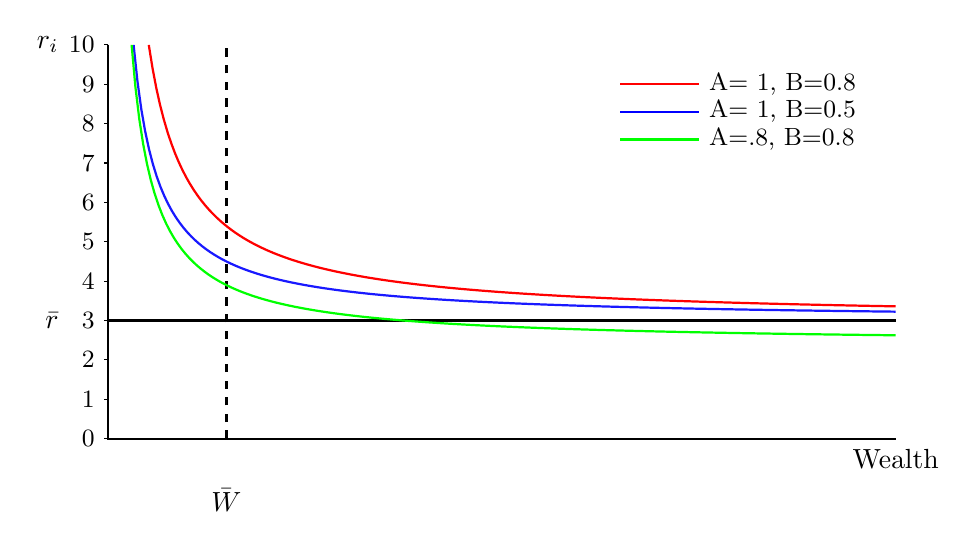
\begin{tikzpicture}[scale=.5]
%\def\bndmax{5}        %https://tex.stackexchange.com/questions/68462/filling-a-complex-region-with-tikz
%\def\bndmin{0.2}
\def \Y {10}  % height of y axis pecent
\def \W {20}  % length  of x axis
\def \Wbar {3} % jmeam wealth
\def \omega {3}
\def \A {1}  %was .5
\def \B {.5}
%Equation   \[ r_i = (A + .5 \frac{\bar{W}}{W_i})\omega\]
\def \Wmin{.63}  %This sets the lower limit fo the 
\def \Wmin{(\B*\Wbar)/(\Y/\omega-\A)} %function to keep in in bounds
	
\tikzset{func/.style={thick,color=blue!90}}	

\draw [thick] (0,\Y)node[left=.5cm]{$r_i$} -- (0,0)--(\W,0)node[below]{Wealth};  	% Axes
\draw [thick] (0,\omega)node[left=.5cm]{$\bar r$} -- (\W,\omega);  	% Axes
\draw [thick,dashed] ( \Wbar,0)node[below=.5cm]{$\bar{W}$} -- (\Wbar,\Y);  	% Axes

\foreach \yi in {0,...,\Y} \draw (0,\yi)--(-.1,\yi)node[left]{\small$\yi$};

\draw[func,domain=\Wmin:\W] plot [samples=200] (\x,{(\A+\B*\Wbar/\x)*\omega});
\def \A {.8}
\draw[func,domain=\Wmin:\W, green] plot [samples=200] (\x,{(\A+\B*\Wbar/\x)*\omega});

\def \A {1}
\def \B {.8}
\draw[func,domain=\Wmin:\W, red] plot [samples=200] (\x,{(\A+\B*\Wbar/\x)*\omega});

\draw [red,  thick](13, 9)--(15,9)node [right, black] {\small A=\ 1,\ B=0.8};
\draw [blue,  thick](13, 8.3)--(15,8.3)node [right, black] {\small A=\ 1,\ B=0.5};
\draw [green, thick](13, 7.6)--(15,7.6)node [right, black] {\small A=.8, B=0.8};
 \end{tikzpicture}
% Figure of cost of borrowing
%\caption{Hypothetical wealth-dependent borrowing cost}
%\label{Fig:BorrowingCost}
%\end{center}
%\end{figure}%

This has a number of immediate implications. First, if agents discount at their borrowing rate, wealthier agents a lower discount rate and therefore value properties more highly. 

Second, given the  common rule that mortgage payments cannot exceed some fraction of disposable income, the wealthy will be able borrow larger amounts and at lower interest rates that the less wealthy. At any distance from the centre they will be able to make a higher bid.
 
If the expected return on a property is greater than the individual cost of borrowing, it would pay any agent to borrow as much as possible and purchase properties as they become available.

\subsubsection{The rate of return on a property purchase $v$}
To explore the implication of the financialization of the urban land market we need a function to calculate the return on a unit of land that reflects the actual gradient of opportunity in financial markets. We begin with the price appreciation, $\Delta P=P_T-P_0 = (1+\dot p)P_0-P_0 $, where $\dot p$ is the rate of price appreciation over the period $T$. Rates will all be specified for the period $T$. Transaction costs, including real estate fees, take a fraction from the value of the final sale.

 The speculator invests a down payment, $D$, and gets back at time $T$ the  increased price $(1+\dot p)P_0$, plus rents, minus any costs and minus the mortgage with interest.
%footnote{We can include a use value, $U$ in place of rent for expatriate owners to represent using the property - say one month a year - when they are not renting the property and a \textbf{vacancy tax},
%$T$ at rate $t$ to affect the speculator's  decision.
 
The rate of return is the value of the gain, $V$,  over the size of the downpayment, $D$, where
\begin{equation}
V =capital\ gain - Interest\ due  	+ Rent  - operating\ cost\    
\end{equation}

The rate of return is $v = \frac{V}{D}$. 

Both the  share of the price  that can be mortgaged, $m$, and the interest rate  and $r$ may be functions of the agent's wealth. $\delta$ represents the net capital gains tax. It makes it possible to capture the capital gains kept. If it is set to one, it simplifies the equations, all is kept. Keeping the variable offers a policy variable to control the return on financial capital.

\begin{eqnarray*}
V  %	&=& capital\ gain - Interest\ due  	+ Rent  - operating\ cost\\
% 	&=& \delta P_T-D \qquad \qquad \quad - (1+\delta r)M \quad	 + R  	-C\\
% 	&=& \delta P _T \qquad-(P_0-M) \quad- (1+\delta r)M 	 + R  	-C\\
%	&=& \delta (1+\dot p)  P_0 -(P_O -M)  -(1+\delta r)mP_0  + R  -C\\
%	&=& \delta (1+\dot p)  P_0 -P_O + M \qquad -(1+\delta r)mP_0  + R -C\\
%	&=&( \delta (1+\dot p)-1)  P_0  + mP_0 \quad -(1+ \delta r)mP_0  + (\rho-\kappa)P_0\\	
%	&=& \left(  \delta (1+\dot p)-1    + m \quad - m(1+\delta r)  + (\rho-\kappa)\right)P_0\\'
%	&=& \left(  \delta (1+\dot p)-1    + m \quad - m-\delta rm  + (\rho-\kappa)\right)P_0\\
&=& \delta(P_T- (1+r)M) \qquad \qquad 	 + R  	-C   - T\\
&=& \delta((1+\dot p)  P_0- (1+r)mP_0)   + \rho P_0  	-\kappa P_0 - tP_0\\
&=&( \delta((1+\dot p)  - (1+r)m) \ + \rho   	-\kappa -t) P_0
\end{eqnarray*}

This is the  net present value of buying, and selling after one period. \textbf{It has  6 exogenous parameters}. Operating revenue and costs $ \rho -\kappa - t$ a present value. 

The rate of return is $v = \frac{V}{D}$. For expat investors, we get a \textbf{decision rule}:\begin{enumerate}
\item  if $v \geq a$ (with some private use?) with no rent,  don't bother renting. 
\item If $v(no\ rent\ and\ tax) < a\leq v(with\ rent)$,  then  rent. 
\item If $ v(with\ rent) \le a $,  then sell 
\end{enumerate}


We can, with some simplifications, write
\begin{eqnarray}
\frac{V}{D}&=&( \delta((1+\dot p)  - (1+r)m) \ + \rho   	-\kappa - t ) \frac{P_0}{D}   \nonumber\\
		&=&( \delta((1+\dot p)  - (1+r)m) \ + \rho   	-\kappa - t ) \frac{P_0}{P_0-mP_0}   \nonumber\\
		&=&\frac{ \delta(1+\dot p  - (1+r)m) \ + \rho   	-\kappa - t } {1-m} \label{Eqn:DecisionRule}
\end{eqnarray}

\subsubsection{Returns on capital are higher for wealthy investors}
\[   r^h=\frac{ \delta(1+\dot p  - (1+r)m) \ + \rho   	-\kappa - t } {1-m}    \]
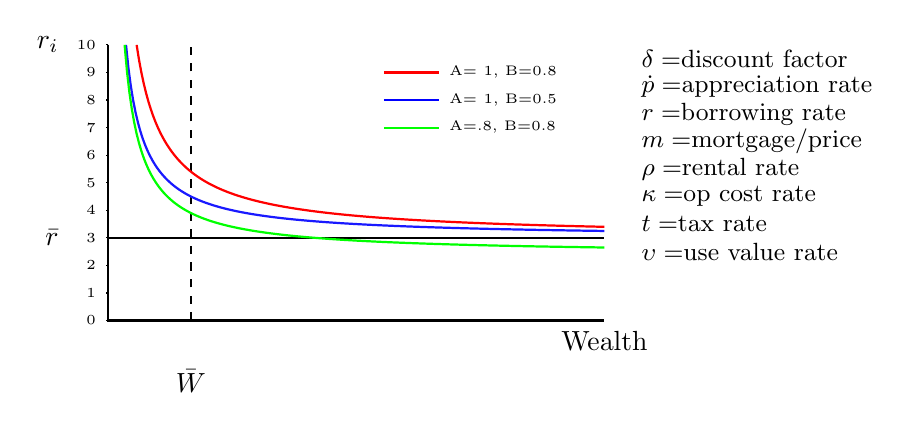
\begin{tikzpicture}[scale=.35]
%\def\bndmax{5}        %https://tex.stackexchange.com/questions/68462/filling-a-complex-region-with-tikz
%\def\bndmin{0.2}
\def \Y {10}  % height of y axis percent
\def \W {18}  % length  of x axis
\def \Wbar {3} % j mean wealth
\def \omega {3}
\def \A {1}  %was .5
\def \B {.5}
%Equation   \[ r_i = (A + .5 \frac{\bar{W}}{W_i})\omega\]
\def \Wmin{.63}  %This sets the lower limit fo the 
\def \Wmin{(\B*\Wbar)/(\Y/\omega-\A)} %function to keep in in bounds
	
\tikzset{func/.style={thick,color=blue!90}}	

\draw [thick] (0,\Y)node[left=.5cm]{$r_i$} -- (0,0)--(\W,0)node[below]{Wealth};  	% Axes
\draw [thick] (0,\omega)node[left=.5cm]{$\bar r$} -- (\W,\omega);  	% Axes
\draw [thick,dashed] ( \Wbar,0)node[below=.5cm]{$\bar{W}$} -- (\Wbar,\Y);  	% Axes

\foreach \yi in {0,...,\Y} \draw (0,\yi)--(-.1,\yi)node[left]{\tiny$\yi$};

\draw[func,domain=\Wmin:\W] plot [samples=200] (\x,{(\A+\B*\Wbar/\x)*\omega});
\def \A {.8}
\draw[func,domain=\Wmin:\W, green] plot [samples=200] (\x,{(\A+\B*\Wbar/\x)*\omega});

\def \A {1}
\def \B {.8}
\draw[func,domain=\Wmin:\W, red] plot [samples=200] (\x,{(\A+\B*\Wbar/\x)*\omega});

\draw [red,  thick](10, 9)--(12,9)node [right, black] {\tiny A=\ 1,\ B=0.8};
\draw [blue,  thick](10, 8)--(12,8)node [right, black] {\tiny A=\ 1,\ B=0.5};
\draw [green, thick](10, 7)--(12,7)node [right, black] {\tiny A=.8, B=0.8};

\def \W {19}  % length  of x axis
\node[right] at (\W,9.5){\small$\delta=$discount factor};
\node[right] at (\W,8.5){\small$\dot p=$appreciation rate};
\node[right] at (\W,7.5){\small$r=$borrowing rate};
\node[right] at (\W,6.5){\small$m=$mortgage/price};
\node[right] at (\W,5.5){\small$\rho=$rental  rate};
\node[right] at (\W,4.5){\small$\kappa=$op cost rate};
\node[right] at (\W,3.5){\small$t=$tax rate};
\node[right] at (\W,2.5){\small$\upsilon=$use value rate};
 \end{tikzpicture}


\chapter{Background Rought Notes - Rent History Etc}



\section{Agglomeration discussion}

The phenomenon of growing productivity was initially identified and estimated in the economics literature production at the national level. The estimated functions linked capital and labour inputs to output.  Soon after the  earliest econometric models of output  were estimated, it was found that equations were not stable over time. Productivity grew over time
(We can do the arithmetic with the cobb douglas to illustrate) 

Faced with this puzzle, Robert Solow introduced a term that was time dependent, and an entire literature developed to explain this term. One productive stream explained growing productivity in terms of agglomeration effects- more people, more workers more firm or more diversity of firms appeared to be associated with growing productivity. Two major schools emerge - roughly speaking,  the Marshallian explanation, which emphasized firm-level processes and the Jacobs model which focuses on the creative effect of agglomerations of people in cities. Both have receives empirical support.

(We can do the arithmetic with the Cobb Douglas to illustrate)

Louis M. A Bettancourt and others applied similar models at the level of cities, but rather than a time-dependent term, they introduced a population-dependent term and found evidence from cities around the world that productivity rose as population rose: The scale of the city has a positive effect. The result  was one of a wide range of scaling results identifies in a great variety of systems examined in the complexity literature 


\section{Background}

\subsection{Inequality}
this wasn't how capitalism was supposed to work
wages part, 
over 50 for rent

\subsection{Drivers of the housing crisis}
supply and demand, stagnant income, and finacialization of housing

Several explanations of the current situation are commonly proposed. The first is simply that the problem of housing is a supply and demand problem where supply is blocked by some features of urban regulation. The second explanation is that the distribution of income has changed in some way that mean a significant fraction of the population are unable to afford satisfactory housing, and therefore this is the problem that must be solved.  The third common explanation currently is that financialization of the housing market  is changing the way the city economy is working, redistributing income and potentially threatening the long term growth and wealth creating capacity of the city.


\subsection{How we do the resilience analysis}

- what will we do? *** 



\section{Rent, Production and the City: Who Gets the Wealth}


%The sources of economic growth and the distribution of income are themes that run through the history of economic thought. 

The story of rent is the story of 

two great theories of distribution
a methodological evolution from descriiption to calculus to complex systems and an evolution of the economy 
from agriculture to indsutrial produciton, to social scaling or wealht in cities. 



There are two great stories of distribution in economics. The first and oldest is rent, %the classical work on rent, going back to 
developed in Ricardo, in which owners of an asset are able to extract a value beyond what they contribute. 
The second is the marginalist approach, developed by Clark and others, looking at a scenario in which workers receive the marginal value of their contribution to production. This tradition dominate in neo-classical economics, particularly in the United States, and %formed the basis of conventional micro-economics training.
% it gave a story of production that seemed to align with the rising fortunes of ordinary people/workers following WWII, in the 1950s and 1960s when it came to dominate. 
% formed an intelectual foundation for anti-monopoly political movements in the early 20th century. 
This work contributes to a third theory of 

emergent complex systems methodology and  work on urban science, the power law concentration, and integrates/ to achieve a sysnthesis of  the clasical descriptive work on rent and the neoclassical marginalist appraoch

These stories are, at their heart, stories of who claims what share of production. They evolved within an evolving theory of production. The early stories of production thinkers like Ricardo focuses on were agricultural. Who claimed the surplus from agricultural production? Over time, the story moved to industrial production, and increasingly urban- with the social wealth of cities/human capacities developed in cities dominating. % Later thinkers including Smith and Marx%leaving aside purely inherited weath- as that becaumse caught in this same circuit of capital transforming from production, to money and back. 



Methodological-- early discririptive theories told rich layered stories with different
The excitiment concentrated  calculus.. in the classical distributional dynamic.

The complexity - allows for tracing the paths of individual- what happens for whom under a far broader range of conditions

The clarity of pedagogical methcs- bottom up and top up both have illustrative cases e.g. edgeworth box or the schellings/birds models.
But true theory integrates in something that moves between scales fluidly, makes itpossible for the distinct scale based approaches to come together.


Complexity

Early discriptive work
This explosion of formal rigour - focused attention.. 


And the political context..

Monopoly- political pressure real explosion ofwealth creation-- economic success of political efforts to break up monopolies.
And a dynamic- lots of worker power- expanded equality-- workers seemed strong, 
As well as the political environment in the US during the cold war, older stories rooted- marx- repression, ednomists perhaps created an envronment in which economists
a side fo the economcs

-- methological pdrived moved the point whre discriptive and historical appraoches baredly taguth.

Samuelson-- successful exciting-- formal-
a generation
created micro, macro
-- at the moment of the baby boom- departments founded in this moment of exuberance. raised in it, taught according to this framework.


Computers took over from calculus -Brian Arthur
Cities took over from industries - concentrated value-- finance- and law main power centers.. - eigen value centrality.

Crisis in 2008 -- reintroduced dscrptive
Methodologial
Cities-- power law dist. rising debt and inequality. -- unstable and financialize.d
Increasing inequality, risind debt. - worker power expanding wages and equality, a story that explained- vs subsistence.


Exactly what those pattnersnew methods are so succesful are what was lef tout..



Polarized in the periodo of the cold war - the discussion of the market-- perhaps a tendency to avoid the distributionl.. Revolution and drama.



Early theories were implicit. They have the same logic- but exist in words

mathematization was important to the simple centrality of marginalism.






With Clark
A second great theory of distribution
The result is much of the theory of rent was lost. 
time

While Marx emphasized the tendency towards consolidation and exploitation in markets, Clark saw the tendancy to increased competition. 

This allocation— dynamic quality of how wages evolved
They are bidding- and it will converge 
What share do workers get- subsistence wages- get 
But as output grows, and as firms compete for labour, particularly skilled labour, is that a sufficient experience.



Three drivers
Calculus had limits.
The political moment of expanding wages with a labour sector in a position to negotiate as the economy rebuilt following WWII and destruction of old wealth— dynamic time. 
Following WWII with growing demand for labour labour could bargain, 
Following WWII in the period— subsistence waves tending— when labour could bargain,
Following break up some of the largest monopolies like in steak— general steal


Also coincided with the political movement McCarthiesm perhaps led scholars to de-emphasize the connections of their work with the classical socialist litturatue.
Mathematical economics became an exciting and dynamic area.

Until this point the theory was largely descriptive..
xx Cobb working with Douglass developed a formulation — exponential, in economics their names have remained associated with the xyz formulation. 

Clark made a case it was just- became problematic.
Doesn't actually happen -- and not jsut

OUR CASE IS THAT IT FALLS OFF A TOTALY DIFFERENT CLIFF



Economics had theories with rich dynamics, concerned 
Classical economics was concerted with ownership and wealth. But they were largely descriptive.
But the new calculus struggled to deal with stocks and with dynamics. 
(Came back with forester and other systems theory, as well as complexity etc.)

The French Engineers in the school of bridge end road used calculus early .. followed by xyz
Technical development and intelleual excitement aligned
Became very exciting dynamic, had many success - took over the discipline. 
Tied with political successes breaking up big monopolies — seemed to offer a path forward

US opposed soviet ideas and an intellectual environment that may have led academics to dephasize the aspects of their thinking connected with classical socialists thought. 

In this environment a particular approach became dominat— also at a moment when schools and departments were growing— the baby boom came to universities at the moment of Samuelson’s peace micro-macro divide gave a tool kit to a whole generation of economists— 

Embedded at the heart of micro- the satisfyingly precise formal structure of calculus.. the marginalize appraoche— 
Thus came to define a new disciplien— a formalization of Econ.. 
Extensions from that base became the defining advances of a generation of American economists..
Attracted math- a feedback loop.

Less emphasis on intellectual history, how changing- heterodox.. all the full range of thought

Including the much more exiting new techniques of complexity and systems- opening in 2007 an explosion of these techniques in the economies. 




CITIES

But cities matter more and more
Jacobs theory of wealth and value as fundamentally social.. 
Combined with xysz. Jacobs did

Now complexity and scaling theory revealing the universality of those principles advanced by Jacobs..

This requires a different formulation of rent… - and production wealth is inherently social what are the implicaitons— what does that mean.. 






In our model, land comes in implicitly through the demand for labour. 


\section{Chapter: Draft Literature Review and Background}

\section{Background}
\label{Sec:Background}
\newpage
Our approach/model is constructed, drawing together pieces from a number of research areas from economics and the study of cities, including rent theory, production functions, the standard urban model, growth theory, urban growth theories, financialization and the theory of distribution. 
We relate this to the scaling models from the study of complexity. This gives a deeper look at distribution in the cities, the effect of financialization, and effect of both of these on the growth and development of cities. 

The literature makes it clear that the cost of transportation is crucial, the cost of housing is crucial, and that there are strong pervasive agglomeration effects driving productivity and population growth. (City population is observed to follow a power law distribution.)

We are interested in agglomeration economies. The wage  structure would then be related to the population or industry  structure. Externalities driving agglomeration may be classified  into two types, the  or so-called ``Marshalian''  and ``Jacobs'' externalities


3 lines  
- production leading to Jane Jacobs
- cities leading to Jane Jacobs
- scaling factors and complexity leading to Jane Jacobs and empirics in a theory of cities

2 theories of production

Ricardo
Ricardo’s rent theory explained class and the distribution of income in terms of the the productivity and ownership of land in an agricultural society. Land was the scarce factor in production and control of land allowed landowners to extract any production in excess of the agricultural wage. Ricardo could assume that labour was in surplus and therefore the agricultural wage would approximate the subsistence wage. 

Marx
Marx adapted the Ricardian model to an industrial society in which surplus product could be used to create more capital and largely ignored land rents. He retained the subsistence wage, and explored the effect of reproducible capital.

Clark
Clark %\footnote{and Wicksteed} extended the theory of rents to produce 
elaborated a neoclassical distribution theory that tied income to the marginal product of each factor for a firm in a competitive economy rather than class ownership of capital. 
This marginal productivity theory became dominant SOME BENEFITS.. Although the marginal productivity theory became dominant in economic thinking, rent theory retained an important explanatory role in resource, agricultural, regional and later urban economics and even sports economics. 

Clark %\footnote{and Wicksteed} %extended the theory of rents to produce 
elaborated a neoclassical distribution theory that tied income to the marginal product of each factor for a firm in a competitive economy rather than class ownership of capital. Although the marginal productivity theory became dominant in economic thinking, rent theory retained an important explanatory role in resource, agricultural, regional and later urban economics and even sports economics. 

Rent theories have remained at the centre of economics despite the development by Clark (1894) of the more modern theory of distribution in which factors ideally receive the value of their marginal product. In modern welfare economics a measure of surplus that is the direct descendent of Ricardian land rent is at the core of the First Theorem of Welfare Economics, arguably the most significant theorem in the social sciences. With Alonso (1964), another another application of rent theory became the foundation of modern urban economics.

\section{Exploitation}
John Roemer’s 1982 Class Exploitation Correspondence Principle (CECP) states that producers who optimize by only selling labour are exploited at the economy’s equilibrium, and agents who optimize by hiring labour are exploiters. Exploitation and class structure are shown to arise from differential endowments in a manner consistent with both Ricardian explanation of class incomes and Marx’s conception of exploitation. We extend the argument to show that differential access to finance capital, urbanization, the growing importance of human capital in producing surplus and agglomeration economies endogenously generate a class structure based on the indirect capture of land rents, We illustrate the emergence of class structure within a simple agent-based model of the land market in a monocentric city. The model is consistent with the theories of Ricardo and Henry George in locating the ground of exploitation and class in the capacity to extract social surplus through land ownership, and differs from the standard Marxian analysis in its reliance on access to financial capital rather than control of productive physical capital.

The sources of economic growth and the distribution of income are themes that run through the history of economic thought. 

From Smith and Ricardo economist have understood that the net product of the economy is divided among functional classes.
 Ricardo is generally credited with providing the best early description for the division of the product of the land between labour and property owners. 
 Marx is generally credited with providing a convincing explanation based essentially on Ricardo's insights, of the distribution of the product of industrial capital with a class-monopoly on ownership the capital,  as well as insights about the evolution of a society based increasingly on produced rather than natural capital. 
 Henry George elucidated the role of land rent, particularly in the urban context as as a mechanism for extracting socially produced economic surplus.  

The division of the product of the earth among the classes of society has been a central issue in economics since at least Ricardo presented his theory of  rent, through Marx, adapted the concept of rent to an industrial and capitalist economy and Henry George, who applied it in the urban context. Land rent is also at the core of modern urban models.  John %\textcite{RoemerGT} 
in \textit{A General Theory of Exploitation and Class} 

%\textcite{RoemerGT} 
%\footnote{\cite{RoemerGT} p12} 

The distribution of rent, where it goes, and what the implications are. 

\section{Liturature Review}

3 lines  
- production leading to Jane Jacobs
- cities leading to Jane Jacobs
- scaling factors and complexity leading to Jane Jacobs and empirics in a theory of cities

2 distributional stories.
- class and rent -- synthesis of rent and class--

Then is the history of rent seperate?

O’Sullivan (2011) identified “five axioms of urban economics” that have emerged from a century of study: (a) location-specific costs and benefits balance to generate a locational equilibrium; (b) self-reinforcing effects induce concentration of activities and individuals; (c) externalities are prevalent; (d) production is subject to economies of scale, which favours agglomeration; and (e) competition generates zero economic profit. These features combine to produce dynamic urban system that will shape our future. 

We build a model that incorporates the five “axioms” to demonstrate how production externalities, in a class of models, can drive urbanization, class formation and the wealth distribution.

To understand the relationship requires integrating the distributional appraoch from clasical economic theory of rent with the modern marginalist model of distribution through wages. It does this by integrating the urban model with the model of production and including the cost of land and transportation in the urban wage in the labour costs. 
In this way the two factor model of projection reflects the clasical landowning extraction of rents by landowners, with a model of wages in competitive markets. 

\subsection{Rent}

 What Is Economic Rent?






neoclassical story.
Economic rent is an amount of money earned that exceeds that which is economically or socially necessary. This can occur, for example, when a buyer working to attain a good or service that is considered exclusive makes an offer prior to hearing what a seller considers an acceptable price. Market imperfections thus lead to the rise of economic rent; it would not exist if markets were perfect, since competitive pressures would drive down prices. 
%https://www.investopedia.com/terms/e/economicrent.asp
% https://www.wallstreetmojo.com/economic-rent/



Henry George brought the classical position to its logical conclusion: rent is an unearned increment. The Classical Base of Modern Rent Theory, Conway L. Lackman
“Whatever part of the produce or… of its price, is over and above this shame” (which pays for the capital advanced “together with the ordinary profits”), “he” (the landlord) “naturally endeavours to reserve to himself as the rent of his land” ([O.U.P., Vol. I, p. 163; Garnier,]  
l.c., p. 300). Theories of Surplus Value, Marx 1861. [Chapter XIV]  
 Adam Smith’s Theory of Rent [1.  Contradictions in Smith’s Formulation of the Problem of Rent]
This excess may “he considered as the natural rent of land” ([O.U.P., Vol. I, p. 163; Garnier,]
l.c., p. 300).


 \subsection{Ricardo}
 
 David Ricardo developed a theory of land rent.
Leading figure in classical economics



He modelled the agricultural economy.
Ricardo developed the idea of 

He was friends with James Mill, Jeremy Bentham and Thomas Malthus.

He theoriezed the agricultural economy.





\section{Drafting REVIEW}
This section traces the history of rent and production in economics.
 central issue in economics since at least Ricardo presented his theory of  rent, through Marx, adapted the concept of rent to an industrial and capitalist economy and Henry George, who applied it in the urban context. Land rent is also at the core of modern urban models.  


In economics, rent is a surplus value, i.e. the difference between the price at which an output from a resource can be sold and its respective extraction and production costs, including normal return (DFID, 2003; Luchsinger \& M\:uller, 2003; Sharp, 2003; Stoneham et al., 2005).

Chapter 24: Doctrine of Adam Smith concerning the Rent of Land
``Such parts only of the produce of land,” says Adam Smith, ``can commonly be brought to market, of which the ordinary price is sufficient to replace the stock which must be employed in bringing them thither, together with its ordinary profits. If the ordinary price is more than this, the surplus part of it will naturally go to the rent of land.

If it is not more, though the commodity can be brought to market, it can afford no rent to the landlord. Whether the price is, or is not more, depends upon the demand.''

More briefly, rent is a surplus value after all costs and normal returns have been accounted for. Normal costs include  payment of all the factors of production at their market rate.(Labour at the going wage, Capital at the interest rate, supplies at their normal price). The great social question at first was who gets the surplus.  

%The question was pressing because it appeared that landlords were capturing the surplus without contributing to production while may peasants were very poor. 

Ricardo

% Born in the late 1700s, was a British poltical economist. The son of a stockbroker, he built a fortune by investing.
The law of rent was formulated by David Ricardo around 1809, and presented in its most developed form in his magnum opus, On the Principles of Political Economy and Taxation. This is the origin of the term Ricardian rent. Ricardo's formulation of the law was the first clear exposition of the source and magnitude of rent, and is among the most important and firmly established principles of economics.

The landlord would rent out all the land which generated at least enough to pay all the costs. Anything in excess of the costs could be charged as land rent to a tenant farmer.

This excess, or surplus, he identified as the income of the landlord. The landlord captures the surplus by ownership of the natural resource land. 

Ricardo, did not write down a production function his, but his analysis can be understood as implying one.

Clearly in his model there are two basic productive factors, land and labour. The landlord  receives the surplus generated by the land and the rest of the value of production goes to labour. Ricardo essentially assumes that there wage is  just sufficient to reproduce the labouring class.\footnote{``In the natural advance of society, the wages of labour will have a tendency to fall, as far as they are regulated by supply and demand; for the supply of labourers will continue to increase at the same rate, while the demand for them will increase at a slower rate.''  This is  basically Malthus.} He has explained the distribution of the fruits of the land among the main classes of the economy.

The implicit production function is
\[Y=F(N, L)\]

Where the output $Y$ is a function of $N$, the number of workers and $L$, land.

His analysis included a concept of diminishing marginal return, the rate at which production grows declines. 
This shows in his use of the terms ``extensive margin'' and ``intensive margin'' to explain the income of the landowner. He focused on the difference between the cost of production on a unit of land and the revenue generated. 



employers enjoy a bargaining advantage over workers and can coerce them to accept worse terms, because they need individual workers less than individual workers need employment. It is no surprise Marx was an admirer. Wages are not the simple product of supply and demand in Smith; bargaining asymmetries are key.

Ricardo included concept of diminishing marginal product, which means


His analysis can be understood in terms of a production function. 
% Factors of production are things that play a role in creating the output. There are several factors of production, things required for production/to create wealth/value (using capital and labour). Most obviously capital and labour. One of the factors of production is labour. In principle the rate at which hiring changes output can take any form. If hiring one more worker increases output, the marginal product of labour is positive. The marginal product can be positive and increasing, or positive and decreasing. If the marginal product of labour is decreasing, the curve is slopes downward, there are decreasing returns to scale, and each additional worker adds less to output than the last. % DIAGRAM  In general hiring more people increases production. In general employers choose workers who would increase production. Otherwise they would not hire. Returns to scale determins how much hiring one more worker increases output. With increasing returns to scale, each new worker increases output more than the last one did, and companies tend to grow big. With decreasing returns to scale, each new worker increases output by less than the last one did and so more, smaller companies may form % (TODO: clarify explanation of implications). To connect with the tradition of analytic economic modelling, ensure there is an equilibrium, by making the marginal product of labour monotonically declining, ors declining over the whole function. This equilibrium condition ensures the curve in the diagram is slopped downward and the curves intersect. % (TODO: discuss/justify assumption, ground empirically)


 2 factors is typical since it's enough for most kinds of analysis. Another factor typically used to introduce another constraint on production, or potentially consumption. Eg. labour is mobile, capital takes time to accumulate but you can put it anywhere, but forest is a flow from the ground-- puts a limit on the region of the city. - land, flow from the land, natural resources.
 
 The factors are usually chosen so xyz
 To keep it tractable- one which is slow to adjust and one which we can adjust quickly - one which is world/embodied work and one which is current work, the rest falls between.

%and is replaced with capital. -- What you'd do an analysis if you put in 30 factors, in the analysis you hold 28 and let 2 move to see what's going on, and what you get is - you have a production function with certain mathematical factors, you can expand as much as you want. you can expand as much as you like-- everything you deduce about 1 is true about any 1 and all the rest if they hold the same functional relation to one another.This is a mathematical trick that gives you xyz.. things you get from it are things like there's a good reason to assume growth till you get 0 profit, then you get competitive markets, all that drops out of the math. - profit maximization you can impose, expansion to 0 profit, expansion till marginal product of labour equals the wage, value of marginal product of capital equals the interest rate, marginal product of whatever is equal to the price/unit of whatever it is - 


Historic evolution is land and labour.

Marx


, as we move from agriculture, 





John Roemer’s 1982 Class Exploitation Correspondence Principle (CECP) states that producers who optimize by only selling labour are exploited at the economy’s equilibrium, and agents who optimize by hiring labour are exploiters.

Roemer
RoemerGT demonstrates that in equilibrium there are classes that are exploited and classes that are exploiters, as well as intermediate cases, using  a definition a definition of exploitation 

that is essentially Marxian and is consistent with Ricardo's rent theory and that of Henry George: 
%\begin{quotation}
%
An agent is exploited  if and only if the value of the labour the agent sells plus the value of own production plus wage earnings is less than the maximum value of their consumption bundle.
%\vspace{.25cm}
%
%and\vspace{.25cm}
%
%An agent is an exploiter  if and only if the value of the labour the agent sells plus the value of own production is less than the minimum value of their consumption bundle.
%\end{quotation}

A General Theory of Exploitation and Class examined a General equilibrium linear economy in which all individuals rationally choose their  activities given their initial endowments and demonstrated  the endogenous emergence of a class structure in a purely neoclassical model. 

Marx
distribution of the product of industrial capital with a class-monopoly on ownership the capital,  as well as insights about the evolution of a society based increasingly on produced rather than natural capital. 



CITY
Rent howerer has remained central in the study of the city
Began everywhere.

Johann Heinrich von Th\"unen was influential in developing the spatial analysis of rents, which highlighted the importance of centrality and transport. Simply put, it was density of population, increasing the profitability of commerce and providing for the division and specialization of labor, that commanded higher municipal rents. These high rents determined that land in a central city would not be allocated to farming but be allocated instead to more profitable residential or commercial uses. 


 Henry George elucidated the role of land rent, particularly in the urban context as as a mechanism for extracting socially produced economic surplus.  

OLD?
 
Ricardo developed a theory of land rent. He did not write down a production function, but he quite clearly understood and used the concept of diminishing marginal product. This shows in his use fo the terms ``extensive margin'' and ``intensive margin'' to explain the income of the landowner. He focussed on the difference between the cost of production on a unit of land and the revenue generated. The landlord would rent out all the land which generated at least enough to pay all the costs. Anything in excess of the costs could be charged as land rent to a tenant farmer.

This excess, or surplus, he identified as the income of the landlord. The landlord captures the surplus by ownership of the natural resource land. 

Clearly in his model there are two basic productive factors, land and labour. The landlord  receives the surplus generated by the land and the rest of the value of production goes to labour. Ricardo essentially assumes that there wage is  just sufficient to reproduce the labouring class.\footnote{ ``In the natural advance of society, the wages of labour will have a tendency to fall, as far as they are regulated by supply and demand; for the supply of labourers will continue to increase at the same rate, while the demand for them will increase at a slower rate.''  This is  basically Malthus.} He has explained the distribution of the fruits of the land among the main classes of the economy.

The implicit production function is

\[Y=F(N, L)\]

Where $N$ is the number of workerrs

\subsection{Marx}
 Marx examined a developing manufacturing economy. In this economy the owners contributed the machinery, buildings, and even working capita to fund the workers until the product can be sold. This contribution must be accumulated from their profits in the preceding cycle of production,  and has to be reinvested once the revenues of the current round have come in and the bills have been paid. Marx actually describes a circuit of capital from its for as money to its form as physical capital. 
 
 
The implicit production function is

\[Y=F(N, K)\]
where $K$ stands for the productive capital stock. 

As in Ricardo, labour is in surplus and capital is scarce. As in Ricardo the scarce factor owned by a special class - now the capitalists, is able to appropriate the is able to capture the surplus value. Like Ricardo,  marx saw the appropriation of surplus as without morel justification - 


Marx also pointed to a new dynamic in capitalist systems - that productive capital is not fixed as land is, but does and must expand as surplus is reinvested. The expansion will eventually outrun the expansion of demand and the rate of return will fall, leading capitalists unwilling to invest and creating a crisis,.


 
\subsection{Henry George} 
  Henry George returned to land rent with a new insight based on the emergence of the capitalist city. Since land rent is unearned income he argued that it should be seen a social income - that it could be used to pay for all the needs of the community. This is the basis of the `single tax' movement. He cleasrly looks back to Ricardo and the early rent theory, but also forward to urban models. His analysis would be recovered in urban models with the proof of. the `Henry George Theorem" in... by .... It demonstrated that if it was some ;public good that attracted people to a city, the optimal level of the good was jus the amount that could be paid for from the increment in land value.\footnote{Progress and Poverty: An Inquiry into the Cause of Industrial Depressions and of Increase of Want with Increase of Wealth: The Remedy is an 1879 book by social theorist and economist Henry George.}
  
  Wikipedia expresses the dynamics this way: ``The tendency of speculators to increase the price of land faster than wealth can be produced to pay has the result of lowering the amount of wealth left over for labor to claim in wages, and finally leads to the collapse of enterprises at the margin, with a ripple effect that becomes a serious business depression entailing widespread unemployment, foreclosures, etc. ''
  
  In George land includes all natural resources, everything ``that is freely supplied by nature.''  
  \footnote{Analysis of the locational rents generated in this class of models has resulted in several authors demonstrating the validity of variants of the Henry George Theorem (\cite{Arnott-Stiglitz79, Arnott04, BehrensKanemoto14, JohnM.Hartwick1980THGR}). These analyses  show that the land rents can exactly equal the cost of the public good that draws individuals to the city or the production services that draws firms. In our model these rents are extracted by land-owning financial capital. They are not invested in a public good or in expanded production capacity.}
  
  \subsection{John Bates Clark}
  Another socialist like George, he was also one of the pioneers of marginalism. By 1986 he was praising the dynamical process of competition partly in opposition to the single tax movement George had initiated.  His (1891). ``Distribution as Determined by a Law of Rent,'' argued that, given  competition and homogeneous factors of production labor and capital, the division of the social product will be according to the productivity of the last physical input of units of labor and capital.\footnote{Responding to the "indictment that hangs over society" that it involves "exploiting labor," Clark wrote:

    It is the purpose of this work (his 1899 'Distribution of Wealth) to show that the distribution of the income of society is controlled by a natural law, and that this law, if it worked without friction, would give to every agent of production the amount of wealth which that agent creates. However wages may be adjusted by bargains freely made between individual men (i.e., without labor unions and other "market imperfections"0, the rates of pay that result from such transactions tend, it is here claimed, to equal that part of the product of industry which is traceable to the labor itself; and however interest (i.e., profit) may be adjusted by similarly free bargaining, it naturally tends to equal the fractional product that is separately traceable to capital.} 
  
 \subsection{Cobb and Douglas}
 The neoclassical revolution opened the use of formal functional mathematics and calculus. Cobb and Douglas (notably Cobb) came up with a specific and very convenient functional form that captured much of what economists were talking about:
 
 \[Y=AK^\alpha L^\beta\]
 
 Where $A$ is a constant scale factor\footnote {apparently previously used by Knut Wicksell, Philip Wicksteed, and L\'eon Walras. I didn't know that!}. The Cobb–Douglas form was developed and tested against statistical evidence by Charles Cobb and Paul Douglas between 1927–1947. It was  the widely circulated empirical work seems to have permanently associated the rather familiar function with the two names for economists.
 
 A 2021 meta-analysis of 3186 estimates concludes that "the weight of evidence accumulated in the empirical literature emphatically rejects the Cobb-Douglas specification."\footnote{Gechert, Havranek, Irsova, Kolcunova (2021), "Measuring capital-labor substitution: The importance of method choices and publication bias", Review of Economic Dynamics, doi:10.1016/j.red.2021.05.003, S2CID 236400765}
 
 The form captured  important regularities in the data but these drifted over time. 
 
 %COBB DOUGLASS additive property-- multiplicative.. additive property-- expandibile in the sense you can add more in-- some functions which are copb douglas which is log linear so seperable, and so additive in an important sense. BUT MVP is true for any firm successfully multipled function even if pruduction function is not seperable..
 
% Write profit using input, profit, - differentiate, get first order conditions which are a peak in the profit function, take those and manipulate to get rules, features of the optimal behaviour-- set marginal value equal to the price, set quantity to the point where profit goes to zero.. approach to standard economics..
 
 \subsection{Solow}
To deal with the drift, Solow introduced a refinement, opening the field for a further series of refinements  in an enterprise that became known as ``growth theory.'' \footnote{A Contribution to the Theory of Economic Growth,  Robert M. Solow, The Quarterly Journal of Economics, Vol. 70, No. 1 (Feb., 1956), pp. 65-94. Stable URL: http://www.jstor.org/stable/1884513}

Solow argued ``As a result of exogenous population growth the labor force increases at a constant relative rate n,'' so
  \[L(t)= L_0e^{nt}\]


 \[Y=A(t)K^\alpha L^{1-\alpha}\]
 where $A$  explains the change in factor productivity as a function of time. It is no surprise that adding a variable allowed the model to track the data better. Solo went farther and described the dynamics of the model using an explicit time dependence: ``As a result of exogenous population growth the labor force increases at a constant relative rate n,'' so
  \[L(t)= L_0e^{nt}\]
  
  
 As a result, if we stick this into the production function 
 \begin{eqnarray}
 Y&=cK^\alpha (L_0e^{nt})^{1-\alpha}\\
    &=c(e^{nt})^{1-\alpha}K^\alpha L^{1-\alpha}\\
    &=A(t)K^\alpha L^{1-\alpha} \label{Eq:Solow}
 \end{eqnarray}
 where
 \[A(t)=c(e^{nt})^{1-\alpha}\]
 
 N. Gregory Mankiw, David Romer, and David Weil created a human capital augmented version of the Solow–Swan model that can explain the failure of international investment to flow to poor countries.

    \[Y(t)=(A(t)K(t)^\alpha H(t)^\beta L(t))^{1-\alpha -\beta} \]
    
    From the Solow example we can see that if all the time functions are exponential we end up with equation~\ref{Eq:Solow} again.
    
\subsection{How the Solow model performed}    
The estimated model explained 78\% of variation in income across countries, the estimates of $\beta$ implied tha t\textbf{ human capital's external effects on national income are greater than its direct effect on workers' salaries.}%(\url{https://en.wikipedia.org/wiki/Solow\%E2\%80\%93Swan_model)}.  
    
This is interesting for me. I got a similar result. Theodore Breton provided an insight that reconciled the large effect of human capital from schooling in the Mankiw, Romer and Weil model with the smaller effect of schooling on workers' salaries. He demonstrated that the mathematical properties of the model include significant external effects between the factors of production, because human capital and physical capital are multiplicative factors of production.[20] The external effect of human capital on the productivity of physical capital is evident in the marginal product of physical capital:

    \[ MPK={\frac {\partial Y}{\partial K}}=\frac {\alpha A^{1-\alpha }(H/L)^{\beta }}{(K/L)^{1-\alpha} }\]
 
 \subsection{Endogenous growth theories}  
 Endogenous growth theories make the increase in factor productivity depend on an optimizing decisions about human capital investment, invention, investment in technology improvement.  
 
  Productivity growth results from an active search process for innovations in
which the ability to appropriate profits determines the resources devoted to
innovative activity (OECD, 1992, Crafts, 1996). Growth depends on the incentives to in-
vest in improving technology.% https://link.springer.com/chapter/10.1007%2F978-1-349-26732-3_13
 
  I don't think these models are much help in understanding cities, which appear to be come more productive and population rises. this is an agglomeration effect.



\subsection{Solow MORE K}

The firm maximizes profit by setting the marginal value of the product of each factor equal to the unit cost per factor. 

This ensures that the marginal rate of technical transformation equals the price ratio. 

*** WHAT IS THE PRICE RATIO

the marginal rate of technical transformation is the (neg) slope of the indiference curve, 
- technical since it's a technology, the production function representws a technology, and you have inputs-- you can maintain one output by substutiting one input for another, you ocan see them as transfromation (substitution)
- changing technology changes the shape of the curve.. ---note growth theories takes technology out of the term-- growth is a term up front.. on avg it's bringing the whole thing up. consistent with the scaling term-- there is this pre factor that changes a lot- e.g. china to US-- 

NOTE AALSO  the pre factor is by nation not just time-- policy matters weath matters, geopolitical context matters.. a. lot. - US is 8x larger than china 27x larger than nigeria (CHECK NUMBERS..) .. bus driver paid x less.


the indifference curve is the curve along which output stays the same as you supstitute labour for capital or vice versa. 
the optimum input mix, it turns out, is where the isoquant (equal quantity - indifference to quantities curve vs indifference to utilities curve) of the production fuction equals output line is tangent to a cost constraint..

curve tangent to a straight line at the optimum-- at the straight line is the price  ratio

the wage over the interest rate. 

ALTERNATIVE FUNCTIONAL FORMS FOR UTILITY FUNCTIONS AND PRODUCTION FUNCTIONS
isoquant measure how things you eat make you happy-- the production function that has that isoquant is measuring equal outputs
vs indifference curve. .. that has the utility-- is measuring happiness, but they are both the same kind of geometric mean of the inputs. 

Examples whrere the isoquant would not euqal the indifference curve include: -- leiontief for instance- right angle corners with 0 substitution . 2 shoes in a pair. need a left and a right one, two right one doesn't help at all. in that case they're perfect complents not subsitutes
if they're straight line, you have perfect substittes a.. 




\subsection{COBB DOUGLASS PROPERTIES}

We use a Cobb Douglass function for production because it has convenient properties -- you can control the degree of degree to return to scale simply by varying alpha and beta. secondly alpha turns out to be under the marginal productivity interpretation of income and optomixation, it ends up being the share of income that goes to capital and to labour- ends up being the elasticity of capital with respect to labour or elasticity of capital with respect to labour.. very much a funcitonal form in line with the scaling  appraoch and they come to the same.. -let's you talk about your returns to scale naturally and ascribe them as you will. it also -- really convenient form used throughout econ for illustration, it has been estimated, and it can be derived alternatively as the form you can look for from the scaling research..]
*** XYZ properties,

cobb douglass has another trait, which is it's a constant elasticity of substitution fuction.
elasticity of subsstittuion combines the slope and the amt of inputs. . easy to slow graphically CEF - constant elasticity of substitution.




Growth theories have several components
the amt of each you have

e.g. if an economy increases the labour or capital it has, it can move to a higher isoquant. if it increases 1 it can move to a higher isoquant-- that doesn't change the shape-- you can move since you have more inputs.

if you have technical change that makes 1 factor more productive.. imagine a nice smooth isoquant.. and it takes some labour that puts you on that isoquant.. if the labour got more producteive, the same amt of labour would move you to a higher isoquant.. cou..


Solow swan puts tech to the front-- the prefactor containts tech growth

we actually put the factor of production into the prefactor.. ** 



% Note on functional form: The analytical approach looks at marginal product and curvature of these functions -- so all we need is something with a curvature and a marginal product in each factor that you put in -time capital, labour 1, labour 2, labour 3.. our focus is on the local curvature and the slope.
%(\cite{Solow56, Swan}), 


VARIATIONS

There are all kinds of other things that could be included in Solow-Swann. For instance, the Mankiw–Romer–Weil version of the model adds a term for human capital.

The general form can be extended in many ways 0 
 In principle it could be restrictred offer time, different workers, firms, sectors, neighbourhooods, evolving over time.


\subsection{Exploitation}\label{Sec:Exploitation: A Note}
The division of the product of the earth among the classes of society has been a central issue in economics since at least Ricardo presented his theory of  rent, through Marx, adapted the concept of rent to an industrial and capitalist economy and Henry George, who applied it in the urban context. Land rent is also at the core of modern urban models. 
%John \textcite{RoemerGT} in \textit{A General Theory of Exploitation and Class} examined a General equilibrium linear economy in which all individuals rationally choose their  activities given their initial endowments and demonstrated  the endogenous emergence of a class structure in a purely neoclassical model. 

%\textcite{RoemerGT} demonstrates that in equilibrium there are classes that are exploited and classes that are exploiters, as well as intermediate cases, using  a definition a definition of exploitation\footnote{\cite{RoemerGT} p12} that is essentially Marxian and is consistent with Ricardo's rent theory and that of Henry George: 
\begin{quotation}

An agent is exploited  if and only if the value of the labour the agent sells plus the value of own production plus wage earnings is less than the maximum value of their consumption bundle.\vspace{.25cm}

and\vspace{.25cm}

An agent is an exploiter  if and only if the value of the labour the agent sells plus the value of own production is less than the minimum value of their consumption bundle.
\end{quotation}

Class position is shown to depend on initial endowments. 
Our model also reveals classes that capture surplus generated by the labour of others. In our model the process is driven by agglomeration economies and urbanization. The analysis does not depend on whether we accept the notion of exploitation presented by Roemer, Marx or any other theorist. We simply note that the model generates classes in a well defined sense, and a division of that surplus among those classes that can be understood  as exploitative in the  classical sense. 







\subsection{Facts justifying our model}

The New Geography of Jobs - what's scarce is tallent. There is catastrophic agglomeration and a growing divide
and those in the good parts cant even afford to own that future, and those outside have no claim even on the income, joy or the chance at a family it offers.

It is debt farmed for ideas till it sheds its' need of you. 
The. actuall needs of humans could sputter out. but what is happening now is simply the draining

the continued logic of extraction.
Tbe logic- it can go somewhere else so ti flows around till place is destroyed. 

the other logic is investment. it looks amost the same. still uses prices, choices, the adjustment so it has alittle more humanity than the naked logic of the individual. -- still spend alone or together. still tu

but the more that stays local the better. and a certain amount stll builds up== the principle builds- the human expression of capacity--

-** all value is craeted for itself. except alienated value. Marx believed the alienation was endemic, but there's a more basic shift in what is needed-- we are needed, at least a few of us as full humans.

--- it is unpredictable

Winner take all-- means everyone gets the best thing. 

The problem of distribution has become the big thing
wealth is connection-- it is the productivity of the dense clusters.. 
Every urban boundary iatrs a potential. we could simply cross the line and install a new logic

1. you'd need a mechanism to drive density- to fight nimbyissm -- the inexorable drive of the markt to unlock an unwillign strivign 
and 
2. you'd need

can we choose a better world ourselves or must we be trappe din it.

of course allow as many other worlds to flourish. most of the world will be free for other worlds so that is no problem.. not even a contracdiction. a new wildness will be on offer, an enw pastoralsim an solw travel airships. 

I have dreamed a few times and cast my webs. played in the eddies of the dancing shimering world as it comes into being. I was at blackberry when it was everywehre, walked in the washinton where it was thew first thing each reached for in the morning and dreamed of the clean lines of the screen ot the edge, the ocmputer. and then held that very thing I'd dreamed of in my hands,

the edge of the inexorable world. anyone can go there and dream and some rutheless one can claim a little share of it.
most will be harvested by the little spiede3rs from law school hwo sit in the corners and and pounce with words never met from it
reality- they are the matrix keepers-- they keep oru constraints in place, they ony thing that takes out enough of our free choice that wecan be predicted and better managed a little

-- it is only the unexpected that is not claimed.
the ghosts of bubbles past.
the hangofers
the feelings never felt

if death iddn't exist we'd invent it
if place didn't exist we'd invent it

we just wiped out something we now have to cojure up but it is just place. a simple thintg not like the dead dancing spiders who well never come back on the odle ear= who will never danc again.
not like the spiders who will never dance in their colours again

come to the museum and see it
be hungry for the flavors adn spices of the world-- see the world -- meet people all over the world killthem.
what can you see, what can you take.

the flowering of the colision
and how few survive it.

but we in the wake of that exploseion. the attom unlocked bust now invent place.

cities were privates.

they are only freed for a moment when they realize that the free mind creates. but it is in a box.

free us all and you can only imagine what we'd make

the pale impovrished publics. the mall is is just a mockery of the public world-- fo the genuine quality of the backyard gathering. 

'Global inequality is not natural, inevitable, or accidental' Jason Hickel The Divide: Global Inequality from Conquest to Free Markets - give aid, they'll get institutions and get rich, but it's a lie of course.
The division is structural.

Have your diversity clubs, but they still cut to the bone, and drive you till your dead. You already adopt an alienated language- runing things up the flag pose. Cliches you'd never dream of in scohol. And so it is just one more thing to control your eyes when the races flash before you on the 'race' tests, just one more false alienated language to adopt. 
And it is all helpsless when it -
and you run farther and farther and still own nothing. Just another day older anddeeper in deblt
But we've sung labour songs for generations. And what we sang is in our bones, it will take more than these false words to cut it off of us. 
I don't want words they say.
I want a way out. I want hope. But even hope smarts, too fresh a promise broken. I cannot vote for hope again, though I cry every time it wins. Another neo-liberal lie

liberalism is this grand dream of liberty and hope. 
But if you don't have the guts
the only dream that cant be co-opted is one that wins.
And it never even tried to win. It never even cared. 


So yes dream of liberty. Drean of truth, and the skyline of forever. But don't dry to me if walking on dreams takes you no-where real.
but don't hit the dreamers.
Hit the liars and the theifs who never gave it a chance.
The ideal was so magical-- so dense, that the worst among it hid in its vabours. 

so densse, lofty diaphanous. Who tood up it's words.
Words. Words. 
The wordy will take them first.

The anti-racist neoliberal beast.
The xx family was the only one to ever embrase the entreprenru.

Great ideas have been peformed. 
And who knows if that's all constatintoble did when he saw the x in the sky and united gentile and jew in the greatest army him history, and binding our god in the. 
But she's free now. The Volcano brought her out. 
And so maybe god is dead. I tried to read him and could get nothing but an empty space.
IT took some time. 
But it is easiery to predict history
But it is easier to predict the future than to say when it will happen

Maybe we can wipe clean our failures now. 
Maybe that slow adoption is ready to speed up.

An emergency is not done by giving up before our time has come. 
Can you make this an experience. 




\subsection{There is an urban rent premium/scaling effect}
There is an urban wage premium %\textcite{HirschJahn} observe that, ``Following \textcite{GlaeserMare}   a  large  empirical  literature  has  investigated differences in wages across labor markets of different sizes. The general finding of this literature is that a significant urban wage premium exists. and that this premium consists both of a level effect and a growth effect that arises as workers gain urban work experience''.

applies most in tech economies like waterloo (maybe also with univerity,   info econ)

applies most with strong urban boundary -- functions essentially as a potential-- could grow with density- urban grows s ti grow the potentieal as well s the wealt-- adds a resilience benefit-- that's why exploiters sees to suc out

scaling laws- socioeconomic outputs scale for the reasons we say.


\subsection{Henry George Results}
Analysis of the locational rents generated in this class of models has resulted in several authors demonstrating the validity of variants of the Henry George Theorem (\cite{Arnott-Stiglitz79, Arnott04, BehrensKanemoto14, JohnM.Hartwick1980THGR}). These analyses  show that the land rents can exactly equal the cost of the public good that draws individuals to the city or the production services that draws firms. In our model these rents are extracted by land-owning financial capital. They are not invested in a public good or in expanded production capacity.

\subsection{Modelling Notes}


simple model justified when there are unknowns % - consider largest uncertainty not just largest data volume - highly available data in part of a model can tempt to complicate a model.. model simplicity should be constriande by the least of data rather than the most. . tend to use all the data we have can unballance

\subsection{How our model compares with other models}

- an origin story, and a test bed-- a grounding that ties it rigorously with the neoclassical model-- 


contrib - a novel intervention, based on a novel theory, recognizing an unusual opportunity- within this region.

contrib - It appears that the analysis of  agglomeration effects has not explored what the endogenous growth literature has to offer.

Production is by firms at the center. The production economy is what generates a surplus.  % This means we have a production/production economy. %, while many models of wealth distibution look at capital and financial markets, 
- vs lots of econo physics models looking at trades/markets rather than production.

Land plays a role in production, but not as a formal factor in the production function, but turns out to be a limit on output. The transportation cost ties labour to land. 

With agglomeration, firms produce more by being near more people.

We put the agglomeration factor in the bracket with labour because agglomeration scales the produtivity of workers.
we actually put the factor of production into the prefactor

The scale litturature comes to the same model with a different derivation, the relationship is traced in Section \ref{Sec:Scale} on Scale. 

 CUT? This differs from  the Slow-Swan, model in which labour augmenting technical change increases according to an exogenous (exponential) - but it's equivalent to the scaling law.

Notice that this model ascribes the agglomeration effects to labour rather than capital. Deepening  and widening of the labour pool was one of Marshall's explanations of the formation of industrial districts. 
The model can therefor  be seen as incorporating a Jacobs/Marshall externality (\cite{Beaudry:2009ua, Panne:2004vb}) of the sort often invoked as an explanation of industrial clusters. 
These externalities  are not a product of any firm or individual, they come from the social interaction of many people.

\subsection{Pictures of the model}

% In Figure~\ref{Fig:Rent1} 
the blue line is a conventional urban rent profile. $A(0)$ represents the effect of including a consumption externality as we do later.  For  $A(0)=0$ the orange line and orange block disappear. 
The social surplus generated by agglomeration effects in production appear as the white triangle below the blue line. The social surplus generated by agglomeration effects in consumption appear as the difference between the blue line and the orange one.
%\begin{figure}[htbp]
%\begin{center}
%\input{SA_RentProfileClasses.tex}
%\caption{Rent profile and population segregation with amenities}
%\label{Fig:Rent1}
%\end{center}
%\end{figure}



% \maketitle \Large

\chapter{A note on the the theory of rent and urban economic development, August 20 2022}

\epigraph{ Alonzo's model has become the standard way  of understanding urban economics. Because it incorporates land rent explicitly, it it can provide the foundation for a  formal analytical approach to the distribution of  the surplus generated generated by an urban system.}

\section{initial notes}
This document describer the link between housing cost, rent theory, and urban prosperity. The analysis has important implications for Ontario Housing Policy and Canadian economic development

The key idea is that cites are productive - they generate a surplus over and above the labour and resources that go into them. We want to understand how the surplus wealth produced by cities is distributed and how it affects the economy.  

It turns out that ownership of land determines  who gets the surplus. Land is a natural resource -- no one creates it. The share or production that goes to landowners is called "rent." To  understand what is happening in our cities we need a basic grasp of  rent theory. To provide that basic understanding, we first very briefly review the familiar supply and demand graph, then show how rent theory is implicit in the model when we apply it to  the ownership of agricultural land. That allows us to show how the basic model of modern urban economic is a variant of Ricardo's model and can be used to approach the question of distribution. Finally we examine some policy implications that follow from the application of rent theory to the current housing crisis.

\section{A preamble}
In 1817 David Ricardo provided the basic economic explanation for the wealth and power of the landowning classes in Britain. Ricardo's insights remain  standard tools of modern economics, although submerged in every first year economics course as consumer and producer surplus, in urban theory as the classic urban rent profile and in institutional theory as  "rent seeking."

Straightforward application of Ricardo's insight using simple supply and demand curves allows us to understand the current housing crisis and the national productivity crisis. It also points the way to a strategy that can solve the housing crisis, make Canadians better off and increase the productivity of the Canadian economy.

\begin{figure}[htbp]
\begin{center}
  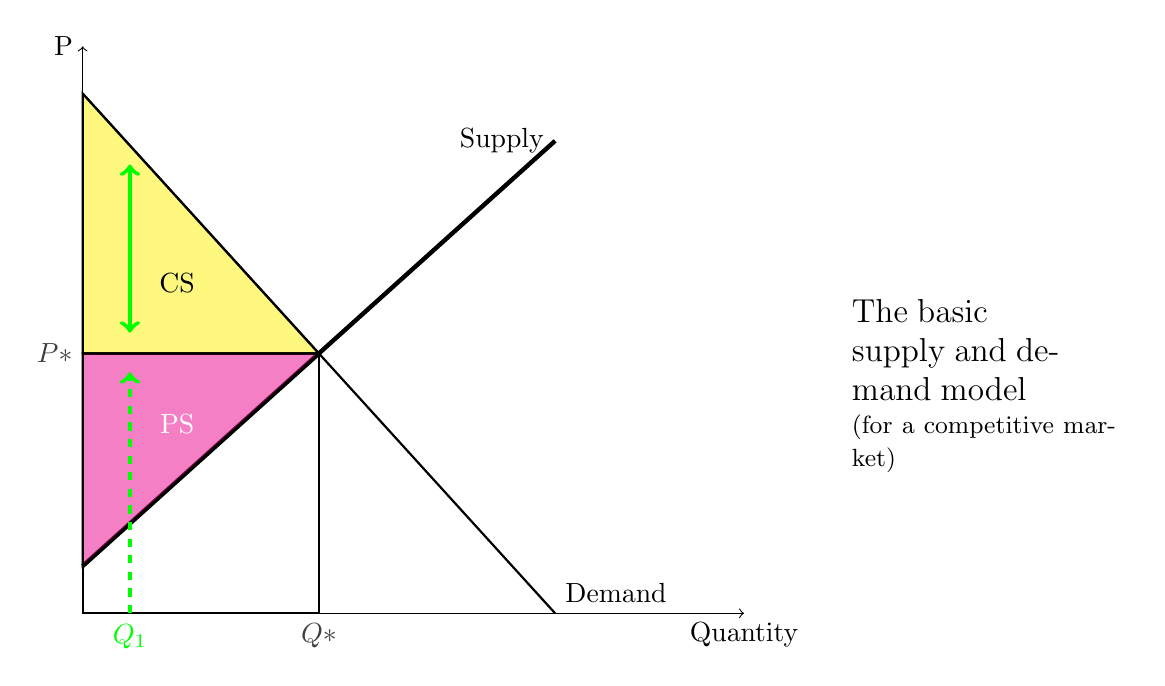
\begin{tikzpicture}[domain=0:2,scale=1.2]        %NINE panesl Top lcr M lcr Blcr
%%%%%%%%%%% 								               TOP%%%     
 %	 \begin{scope}[scale=.6, shift={(6,20.5)}]  % Tr : features of S and D 
			%  \draw [gray] (0,0) grid (7,7);
		\draw [<->] (0,6)node[left]{P} -- (0,0) -- (7,0)node[below]{Quantity};
  
		\draw [thick] (0,5.5) -- (5,0)node[above right]{Demand};
	%	\node at (5,0)[below]{$Q_{max}$};
		\draw [ultra thick] (0,.5) -- (5,5)node[left]{Supply};
				 
		 \draw [thick, fill opacity=0.75] % fill=yellow,
		 		(0,0) -- (0,2.75) node[left]{$P*$}--(2.5, 2.75) --(2.5, 0)node[below]{$Q*$} -- cycle;
 		\draw [thick, fill=yellow, fill opacity=0.5]  
				(0,5.5) -- (0,2.75) --(2.5, 2.75) -- cycle;
 		\draw [thick, fill=magenta, fill opacity=0.5]  
				(0,.5) -- (0,2.75) --(2.5, 2.75) -- cycle;

		 \node at (1,2) (b) [white] {PS};
		  \node at (1,3.5) (b) [black] {CS};

	\draw [ultra thick, green, <->] (.5, 4.75) -- (.5, 2.97);
	\draw [dashed, ultra thick, green, ->] (.5, 0)node[below]{$Q_1$} -- (.5, 2.55);

  \begin{scope}[scale=.6, shift={(10,0)}] 
		    \node at (6,4) (b) [black, text width=3.5cm] {\large The basic \\supply and demand model\\ {\small (for a competitive market)}};
\end{scope}		    
\end{tikzpicture}
\caption{The basic supply and demand graph}
\label{Fig:SDFigure}
\end{center}
\end{figure}

\section{Basic Supply and Demand}
Although the basic supply and demand graph had not been invented in Ricardo's time, we can use it to illustrate the Ricardo's insights. In Figure~\ref{Fig:SDFigure}, the height of the demand curve at each quantity represents how much buyers will pay for  one more unit of whatever is being sold in this market. The height of the supply curve is the cost of producing one more unit. Producers won't want to sell any units that cost more than they are being paid.

To read the graph, we can pick a price, and read horizontally to the demand curve to `predict' how many  consumers  want to buy at that price, and across  the supply curve to find out how many producers want to sell. If they don't agree on a quantity to transact, we say ``the market doesn't clear.''  At the price $P*$, where the curves cross, however, they will agree on quantity, so we'll assume the this becomes the market price.

The graph doesn't just describe buyer and seller behaviour leading to a market price and quantity. It can also measure the social benefits produced by the private market. Some  buyers would have bought the product even at a price higher than the market price. The difference  between the price they pay and the the price they were wiling to pay is an \textbf{economic surplus}.  The solid green arrow in the yellow area of the figure is the amount of this excess benefit called   `consumer surplus' received by whoever bought unit $Q_1$. The yellow area is the sum of consumer surplus of all buyers. 

Similarly, the magenta area below the price line is what economists call "\textbf{producer surplus}" -- the difference between the sale price and the \textbf{marginal} cost of production. It is not profit because most producers still have to pay the costs of producing capital goods. Fixed costs have to be deducted. 


%Overall, the supply and demand graph  is a remarkably simple  model that lets us think clearly  the behaviour of hundreds, or even millions, of two different kinds of people, the buyers and sellers, when they interact. It finds a combination of price and quantity that is likely to be reasonably stable, and it can be applied to all kinds of markets. 

\section{Ricardo's problem}
In agriculture the cost of producing land is zero. Land is a "free gift of nature''. As a result, agriculture in the entire producer surplus is available to distribute. Ricardo didn't call it producer surplus, however. That term had not been invented. He used a term that was already applied to the agricultural surplus: \textbf{rent}.

 Ricardo's theory  explained how the surplus produced by the land was shared between landowners and labour. We can adapt the supply and demand  model to describe what Ricardo discovered.  
 
\begin{figure}[htbp]
\begin{center}

  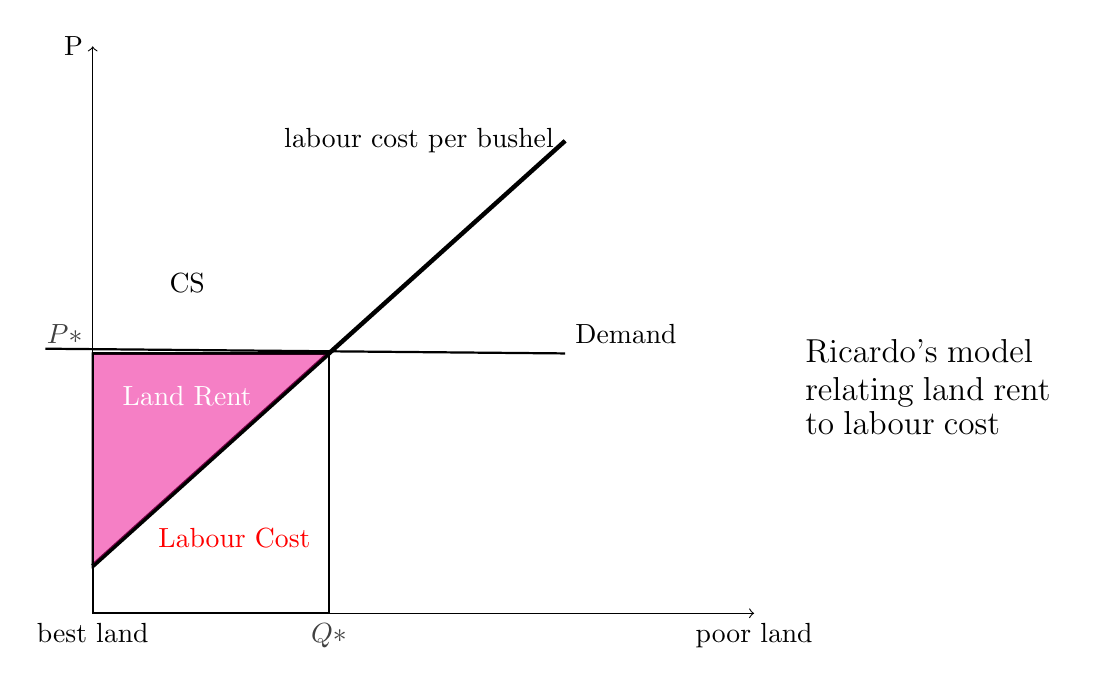
\begin{tikzpicture}[domain=0:2,scale=1.2]        %NINE panesl Top lcr M lcr Blcr
%%%%%%%%%%% 								               TOP%%%     
 %	 \begin{scope}[scale=.6, shift={(6,20.5)}]  % Tr : features of S and D 
			%  \draw [gray] (0,0) grid (7,7);
		\draw [<->] (0,6)node[left]{P} -- (0,0)node[below]{best land} -- (7,0)node[below]{poor land};
  
		\draw [thick] (-.5,2.8) -- (5,2.75)node[above right]{Demand};
		%\node at (5,0)[below]{$Q_{max}$};
		\draw [ultra thick] (0,.5) -- (5,5)node[left]{ \normalsize  labour cost per bushel};
				 
		 \draw [thick, fill opacity=0.75] % fill=yellow,
		 		(0,0) -- (0,2.75) node[above left]{$P*$}--(2.5, 2.75) --(2.5, 0)node[below]{$Q*$} -- cycle;
 	%	\draw [thick, fill=yellow, fill opacity=0.5]  
				(0,5.5) -- (0,2.75) --(2.5, 2.75) -- cycle;
 		\draw [thick, fill=magenta, fill opacity=0.5]  
				(0,.5) -- (0,2.75) --(2.5, 2.75) -- cycle;
				
 		 \node at (1.5,.8)  (a) [red] { \normalsize Labour Cost};
		 \node at (1,2.3) (b) [white] { \normalsize Land Rent};
		  \node at (1,3.5) (b) [black] {CS};

	%\draw [thick,dashed] (.5,7) -- (.5,0)node[below]{$Q_{low}$};


  \begin{scope}[scale=.6, shift={(10,0)}] 
		    \node at (5,4) (b) [black, text width=3.5cm] {\large Ricardo's 
model\\ relating land rent\\ to labour
cost};
\end{scope}		    
\end{tikzpicture}
\caption{Ricardo's Figure}
\label{Fig:Ricardo'sFigure}
\end{center}
\end{figure}


 In Figure~\ref{Fig:Ricardo'sFigure}, the height of the supply curve from Figure~\ref{Fig:SDFigure}   becomes the labour cost of producing  `corn' (we call it wheat now) on each plot of land, from best on the left to the worst on the right. Naturally cost in labour rises as we move to less productive. The supply curve now shows the rising cost as more land is planted.
 
 Since Ricardo was  just dealing with the production side and assuming that landowner and peasant knew roughly what  price would be paid for `corn' (we call it wheat now), we can  draw the demand curve for  Figure~\ref{Fig:Ricardo'sFigure} as a horizontal line and w e can ignore consumer surplus.

Landowners didn't actually farm, and they didn't usually hire workers to farm the way that an industrial capitalist did. They rented plots land to peasant farmers.  Maximizing their rent  income meant minimizing the share of the surplus that the peasants got to keep. Since land was scarce and peasants were numerous, the landlord generally had the upper hand and could squeeze out something close to the maximum rent.\footnote{After the black death there were fewer peasants  and they were able to negotiate lower rents}. Peasants got paid for their labour, often just a subsistence wage, and landowners captured all of the surplus in Ricardo's theory.

%Landowner and peasant knew roughly what  price would be paid for `corn' (we call it wheat now) when it was produced, how much corn a particular plot would produce, and how much work it would take to produce that corn. Although the rent-setting process was probably quite different, we can imagine the peasant knowing the maximum he would bid to farm a particular lot.  We can imagine the peasant and the landlord negotiating over the rent. 

\section{Modern Urban Economics}
Bid rent theory\footnote{Location and Land Use, (1964) by William Alonso.} is a geographical economic theory that refers to how the price and demand for real estate change as the distance from the central business district (CBD) increases.\footnote{von Th\"unen's The Isolated State (1826) generates a pattern of agricultural land use based on transportation costs and can be seen as synthesizing Alonzos and Ricardo's insights. } It is essentially Ricardo's rent theory, except that the figure is turned upside down and labour cost  is replaced with transportation cost, as in Figure~\ref{Fig:Alonzo'sFigure}. 

In this model, workers demand land that provides access to wage employment at the core. Their willingness to pay -- their bid rent -- is lower for land farther from the core because the transportation costs eat up some of the wage. 

As in Ricardo's model, landowners capture the land rent.  Urban tenants are in the same position as Ricardo's tenant farmers with respect to land rents. Like freehold farmers, owner occupiers capture the land rent  for their own property.


\begin{figure}[htbp]
\begin{center}

  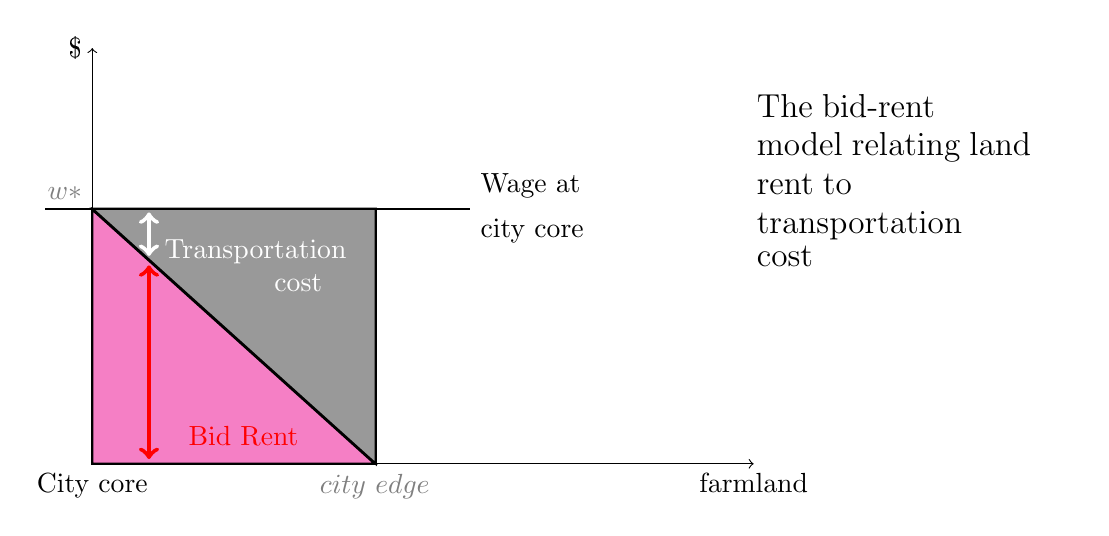
\begin{tikzpicture}[domain=0:2,scale=1.2]        %NINE panesl Top lcr M lcr Blcr
%%%%%%%%%%% 								               TOP%%%     
 %	 \begin{scope}[scale=.6, shift={(6,20.5)}]  % Tr : features of S and D 
			%  \draw [gray] (0,0) grid (7,7);
\draw [<->] (0,4.4)node[left]{\$} -- (0,0)node[below]{City core} -- (7,0)node[below]{farmland};
\draw [thick] (-.5,2.7) -- (4,2.7)node[above right]{Wage at}node[below right]{city core};
				 
 \draw [thick, fill=magenta, fill opacity=.5] 	(0,0) -- (0,2.69) node[above left]{$w*$}--(2.99, 0)node[below]{$city\ edge$} -- cycle;
\draw [thick, fill=black, fill opacity=0.4]  (0,2.7) -- (3,0) --(3, 2.7) -- cycle;
				
\node at (1.6,.3)  (a) [red] { \normalsize Bid Rent};
 \node at (1.6,2.1) (b) [white, text width=2cm, align = right ] { \normalsize Transportation cost};

\draw [ultra thick, white,< ->]    (.6, 2.2)-- (.6, 2.66);	
\draw [ultra thick, red, <->] (.6, .05) -- (.6, 2.1);



  \begin{scope}[scale=.6, shift={(10,0)}] 
		    \node at (4.5,5) (b) [black, text width=4cm] {\large The bid-rent \\model relating land  rent to \\transportation\\ cost\normalsize};
\end{scope}		    
\end{tikzpicture}
\caption{The bid-rent model}
\label{Fig:Alonzo'sFigure}
\end{center}
\end{figure}
 Alonzo's model has become the standard way  of understanding urban economics. Because it incorporates land rent explicitly, it it can provide the foundation for a  formal analytical approach to the distribution of  the surplus generated generated by an urban system.
  


\chapter{Glossary}

Rent: facility,  variously defined as a category of income, payment for the use of a facility,  the income accruing to the owner of land,  the surplus that can be ascribed to a non-produced and finite resource, and a social relations among classes

Stylized fact


 
scaling law





% \part{A Model of Financialization and Rent}
% Density- this creates reant

% \part{Systems Analysis}


% \part{Other}

% 
\maketitle \Large

\chapter{A financial model for making housing affordable}

\epigraph{ We considered the dynamics and impacts of a publicly supported coop model designed to produce
two million housing units over five years}

\section{Solutions}
\subsection{Why it is necessary to intervene in the Housing market }
Canada is projected to attract at least 1.3 million immigrants over three years.
\footnote{The  \href{https://www.canada.ca/en/immigration-refugees-citizenship/corporate/transparency/committees/cimm-feb-15-17-2022/2022-2024-multi-year-levels-plan.html}{022-2024 Immigration Levels Plan, tabled on February 14, 2022} specifies   431,645 in 2022 (range: 360,000-445,000),     447,055 in 2023 (range: 380,000-465,000),     451,000 in 2024 (range: 390,000-475,000).} 
At that rate population will rise by 4-5 million by 2030. To put these numbers in perspective, Canadian cities with a population of 100,000 to 1 million are considered medium-sized, 

 CMHC has conservatively 
 \href{https://www.cmhc-schl.gc.ca/en/blog/2022/canadas-housing-supply-shortage-restoring-affordability-2030}{estimated} 
 estimated that If the current rates of new construction continue, the housing stock will increase by only 2.3 million units between 2021 and 2030. 
 
 To restore affordability, an additional 3.5M affordable housing units are needed by 2030 3.5M affordable housing units will be needed by 2030, bringing the total required to 5.8 million units.  CMHC therefore  calls for ``a drastic transformation of the housing sector, including government policies and processes, and an ‘all-hands-on-deck’ approach to increasing the supply of housing to meet demand.''  The challenge is to produce approximately 4 million affordable units that the housing market as currently organized will not provide. 

The analysis in this thesis concludes that, given the ongoing financialization of the housing market, which is not considered in the CMHC analysis,

\begin{enumerate}
\item the financial system will eventually extract all net urban land rents through investment in urban property
\item housing accessibility will become increasingly challenging for disadvantaged groups
\item housing will be largely eliminated as a saving mechanism and asset fr middle income Canadians,  resulting in a systematic decline in the `middle class'
\item that the quality of urban life will decline
\item the economic growth and development of cities is threatened by this financialization
\end{enumerate}



\subsection{An institutional approach to the inevitable failure of the existing market mechanisms}

 In this note/section/chapter we describe a financial model with several desirable properties
 
 \begin{enumerate}
     \item land rents will be shared with a growing fraction of residents through cooperative housing structures, rather than captured by a declining number of homeowners and asset holders
     \item social housing and land ownership will expand
     \item the rising cost of housing will be ameliorated
     \item economically disadvantaged groups will enjoy increase access to affordable housing.
     \item the quality of housing will improve
     \item society's ability to respond to climate change and to engage in land-use planning will improve     
 \end{enumerate}


 It is our contention that all of these objectives can be achieved with existing institutions and relatively simple, though dramatic, public interventions.

 The instrument that has most potential for solving the growing housing crisis is the cooperative movement. Co-operative housing represents an important part of the housing market in many countries in Europe and clearly have the potential to operate at the necessary scale in Canada. . For example, housing co-operatives currently manage over 3.5 million dwellings in Poland (about 27\% of the total housing stock in the country in 2009), about 17\% of the total housing stock in the Czech Republic and Sweden, 15\% in Norway.
 \footnote{\href{https://coopseurope.coop/cooperative-housing-key-model-sustainable-housing-europe-organised-cecodhas-housing/}{Cooperatives Europe}}

 A housing cooperative is a housing business in the form of a consumer cooperative mutually owned by its members, which operates in accordance with the Cooperative Principles and Values. 
 \footnote{https://www.ica.coop/en/cooperatives/cooperative-identity}
  It is centered around a cooperative of inhabitants that collectively develops, finances, maintains and operates multi-resident projects. This make the cooperative structure  especially appropriate for what we have called the `shoulder' of the urban core - the area of low density, usually single-family housing on the edge of the high-density, multi-unit areas on modern cities. 
 
 There is wide agreement that raising the density in these areas is necessary part of any housing strategy. The bulk of new housing over the next 40 years will be created in these `shoulder' areas. That should makes this class of multi-family housing the main target of Canadian housing policy. 
 
 Because it controls  does not need to make profit, coop housing can be much more affordable. Challenges remain if coops are to be a large-scale instrument of housing policy however. 
 
 \begin{itemize}
     \item Coops are a corporate form of housing and land ownership. As a result speculative gains accrue to the membership, making the conventional housing cooperate useless as a mechanism for capturing the socially produced capital gains for the community as a whole.
     \item Coops are not inherently inclusive although they may seek to expand their membership. They are designed to benefit only members. 

     \item Coops, like privately owned housing with rent-control, may inhibit mobility, reducing community productivity.
     \item Coops, like rental housing, generally do not allow residents to accumulate    `sweat equity', an important savings mechanism for  households.
     \item Individual coops are generally small scale, very local organizations, limiting their impact.
     \item Although credit risk is assumed by the cooperative  (a more robust approach than individual financing), coops do not have access to funds at preferential public sector rates
    % \item 
 \end{itemize}

 \hrule
\color{SeaGreen}\vspace{1cm}
\begin{quotation}
\section*{The MOBA* housing model}

The \href{https://moba.coop/}{MOBA housing model}  is centered around a cooperative of inhabitants that collectively develops, finances, maintains and operates a multi-apartment building. Because it controls the entire trajectory (and does not need to make profit), the resulting apartments are much more affordable for the inhabitants. 


The cooperative owns the real-estate as well as takes on the necessary loans to pay for its construction. Participating households or individuals (the members of the cooperative) thus collectively own their building. Individual members or households cannot speculate with their apartment or their stake in the land – in that way it is not just a safe and affordable option for the first generation, but for many generation of its inhabitants to come.  


\tiny * A network of housing cooperatives from Belgrade (Pametnija Zgrada / Ko Gradi Grad), Budapest (R\'ak\'oczi Collective),  Ljubljana (Zadrugator), Prague (Sd\'ilen\'e domy / První Vlaštovka) and Zagreb (Cooperative Open Architecture)  with support from the Cooperative for Ethical Financing (ZEF), urbaMonde, World Habitat, Socialni inovatori, FairCoop and Heinrich B\"oll Foundation.\normalsize

 \end{quotation}
 \vspace{1cm}
 \hrule
 \color{black}

\newpage
\section{A model}
 \textbf{We will examine the dynamics and impacts of a publicly supported coop model designed to produce two million housing units over five years} In our view this is the appropriate design scale for hte project. 

 We begin by specifying the features of a National Housing Cooperative needed to make the project work.

 \begin{enumerate}
     \item The coop is national, and members have the right to apply to transfer to vacant or new units anywhere in the country. This provides \textbf{improved labour mobility}, clear market signals for development and improved household freedom, and reduced transaction costs for households.
     \item individual housing payments can be linked to local market rents, encouraging efficient use of the housing stock. 

     \item  as  individuals join they contribute equity to the coop for the construction of new housing. The coop thus mobilizes household saving effectively. 
 \item individual housing payments are offset by a fair return on the  housholder's equity. 
    \item individual equity may be augmented through social programs based on the right to housing and a national housing-first strategy. 
    
     \item total coop equity is divided between individual member equity and common equity. The coop owns all equity in the land and is a co-investor in each housing unit. 
     \item The coop captures all capital gains on land a part of the capital gains on buildings. The gains are directed to expansion of the housing stock, with some used to keep the cost of housing low.
     
 
     \item public sector land is made available to the cooperative (ideally no public sector land that might eventually be used for housing is allowed to pass into private hands) on the condition that it remain in the non-profit housing cooperative forever be converted to public housing. 
     \item to finance rapid and large-scale coop housing governments lend to the cooperative at the lowest possible public borrowing rate taking as security the assets of the cooperative. In effect there is no addition to net debt for the government. The government does take on some financial risk, as it does with, for example student loans.
     \item all public housing funds, including all CMHC lending  are channeled thought the cooperative. The result is that the public sector ceases entirely to subsidize private. ownership of housing and the concomitant speculative gains for individually.
     \item Since the government has historically subsidized housing, the governments of Canada commit to a universal basic housing grant which may only be used to purchase coop membership and housing. Home-owners would be excluded from this grant on the grounds that they have benefited from prior subsidies and unearned captial gains.
     \item  
     
     \end{enumerate}

     
\section{Advantages of the model}

A feature of this model is that it can combine the advantages of scale in financial management and project development while including local design and responsiveness to member needs.

The model will gradually build a non-market housing  sector that will provide an attractive alternative to pure market housing and will eventually moderate rent increases across the syste.

The model will produce the ``missing middle'' types oh housing because members will participate in design and financing. at t he same time it will be able to exploit  all of the economies of multifamily projects. 

The model will provide a platform for ecological planning, since residents will participate in development and management. This link is almost always absent in developer-built housing.

Public land and, for example, church lands, can legitimately be committed to the cooperative because the land remains a community asset.

The model is able to get `public license' for developments - \begin{itemize}
    \item to use public land
    \item to receive subsidies for the homeless, the poor, and the young
    \item enter into neighbourhood. The price of the risk of failing to get social license for a project is a significant cost (10\%) that these projects can avoid even when they have the same building costs.  Government investment, participation of local residents, guaranteed  tenure structure. This can allow development in the areas where it is most valuable. Existing residents can participate in planning that improves their own property values
\end{itemize}

\section{The moment}
with rising interest rates, a public intervention. can give the entire coop sector a relative advantage in financing. 






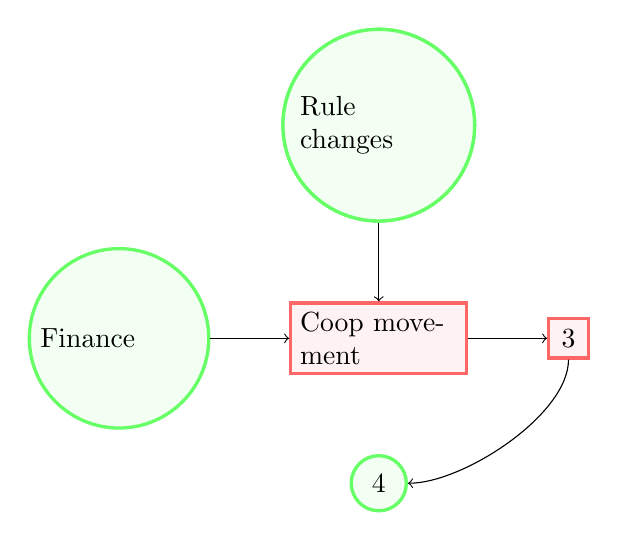
\begin{tikzpicture}[
roundnode/.style={circle, draw=green!60, fill=green!5, very thick, minimum size=7mm},
squarednode/.style={rectangle, draw=red!60, fill=red!5, very thick, minimum size=5mm},
]
%Nodes
\node[squarednode, text width= 2cm] (Coop)          {Coop movement};
\node[roundnode, text width= 2cm, text width= 2cm]  (uppercircle)       [above=of Coop] {Rule changes};
\node[roundnode, text width= 2cm, text width= 2cm]  (leftcircle)       [above=of Coop] {Rule changes};

\node[roundnode, text width= 2cm, text width= 2cm]  (leftcircle)       [left=of Coop] {Finance};

\node[squarednode]      (rightsquare)       [right=of Coop] {3};
\node[roundnode]        (lowercircle)       [below=of Coop] {4};

%Lines
\draw[->] (uppercircle.south) -- (Coop.north);

\draw[->] (leftcircle.east) -- (Coop.west);

\draw[->] (Coop.east) -- (rightsquare.west);
\draw[->] (rightsquare.south) .. controls +(down:7mm) and +(right:7mm) .. (lowercircle.east);
\end{tikzpicture} % TODO add back
% 


\chapter{Lifeboat Canada}

\epigraph{ Canada must develop a humane housing strategy that supports rapid population growth, social integration and economic productiveness.  This is clearly a large-scale system design problem.}

\section{External forces}
Canada's current housing crisis and the projections of the previous chapter are mild compared to what we may face as the globe warms. Canada has committed to admitting  1.3 million immigrants over three years.   %Meanwhile housing  affordability has been declining since 2003-4, especially in Ontario, Alberta and BC.
If external world conditions remain as they are, the number of immigrants is likely to rise through the coming century. An annual increase of just  1\% each year (slightly less than the  rate of population growth for the last 50 years)  will raise immigration to nearly one million per year by the end of the century. The current growth is equivalent to adding one to four medium sized cities per year. That number will rise to as many as nine medium sized cities or one large city per year at the end of the century.   

External world conditions will not remain as they are, however.  According to a \href{https://www.pnas.org/doi/10.1073/pnas.1910114117}{study in the journal Proceedings of the National Academy of Sciences}\footnote{Future of the human climate niche, Chi Xu, Timothy A. Kohler, Timothy M. Lenton  Jens-Christian Svenning, and Marten Scheffer, May 4, 2020, 117 (21) 11350-11355.  https://doi.org/10.1073/pnas.1910114117}, the planet could see a greater temperature increase in the next 50 years than it did in the last 6,000 years combined. By 2070, the kind of extremely hot zones, like in the Sahara, that now cover less than 1 percent of the earth’s land surface could cover nearly a fifth of the land, potentially placing one of every three people alive outside the climate niche where humans have thrived for thousands of years. The result will be large scale migrations to the shrinking band of habitable lands.% A change in the geographical distribution of human populations  is  likely part of the spontaneous or managed adaptive response of humanity to a changing climate

Temperature will not be the only source of migration pressure. Kulp1 and Strauss\footnote{Kulp, S.A., Strauss, B.H. New elevation data triple estimates of global vulnerability to sea-level rise and coastal flooding. Nat Commun 10, 4844 (2019). https://doi.org/10.1038/s41467-019-12808-z} show – employing NASA’s nes Digital Elevation Model, CoastalDEM, that 190 M people (150–250 M, 90\% CI) currently occupy global land below projected high tide lines for 2100 under low carbon emissions, up from 110 M today. Under high emissions, CoastalDEM indicates up to 630 M people live on land below projected annual flood levels for 2100, and up to 340 M for mid-century.

Extreme weather events and conflict are the top two drivers of forced displacement in the short run globally. Since 2008, according to the United Nations High Commissioner for Refugees (UNHCR), an annual average of 21.5 million people have been forcibly displaced by weather-related events – such as floods, storms, wildfires and extreme temperatures.\footnote{https://www.unhcr.org/uk/news/latest/2016/11/581f52dc4/frequently-asked-questions-climate-change-disaster-displacement.html.  See also Gaudry Haynie, J., Balagna, J., clark-Ginsberg, A. (2021) “Climate Change Migration: Developing a Security Strategy for All,” (https://www.rand.org/blog/2021/03/climate-change-migration-developing-a-security-strategy.html) who give suggest that nearly 30 million people  are displaced by weather and  conflict each year. Cited in the White House REPORT ON THE IMPACT OF CLIMATE CHANGE ON MIGRATION, October 2021. } The Institute for Economics & Peace (IEP)  predicts that 1.2 billion people could be displaced globally by 2050 due to climate change and natural disasters.\footnote{https://www.prnewswire.com/ae/news-releases/iep-over-one-billion-people-at-threat-of-being-displaced-by-2050-due-to-environmental-change-conflict-and-civil-unrest-301125350.html}. It is difficult to find anyone willing to make forecasts for the rest of the 21st century.\footnote{Projections assume that there will not be a mass die-off in this century as forecast by the 12972 Club of Rome Report, Limits to Growth", if society continued, as it has, on the ``Business as Usual'' path. }  



Canada, with its huge land-mass, relatively mild climate, stable government, high standard of living, and extensive agricultural capacity will be a preferred destination for many migrants. With perhaps one quarter of the most attractive land on earth at the end of the century, Canada is likely to receive or to be under  pressure to receive, a disproportionate share of global cross-border migration. It is unclear how many of those affected will look to Canada. An article in the UN Chronicle argues that, for several reasons,  it is ``improbable that there would be long-distance mass population movements even in a situation of systemic climate change.''\footntoe{https://www.un.org/en/chronicle/article/will-there-be-climate-migrants-en-masse}  Displaced people tend to stay near their origins, refugee camps and shelter villages are typically set up not far from the site of the calamity, countries resist cross-border migration, and various forms of adaptation are possible.  

Nonetheless, there is little doubt that Canada will have the opportunity as well as pressure to settle significantly larger numbers that currently envisioned. 
The country will face \textbf{the classic lifeboat problem}  described by by Garrett Hardin:\footnote{\textbf Garrett Hardin, BioScience Vol. 24, No. 10 (Oct., 1974), pp. 561-568 } how many are allowed aboard the lifeboat?  How many can the lifeboat sustain? how many will be left to die?

Faced with this dilemma, Canada can treat the situation as an opportunity to draw in far more talented and productive immigrants  than currently planned. 
 %Furthermore,  humanitarian considerations provide another motive for accepting far larger numbers of migrants.
The carrying capacity of \textbf{Lifeboat Canada}, however, depends on actions taken now - Will Canada have the capacity to house larger number of  immigrants given its difficulty in housing its current population?  Will Canada be able to integrate larger numbers into its economy? Will the country be prepared to quickly mobilize  the creative power of immigrants.

\section{The design challenge}
To prepare \textbf{Lifeboat Canada} for the opportunity and 
potential threat of mass migration and greatly increased immigration, Canada must develop a housing strategy that supports rapid population growth, social integration and economic productiveness. The strategy must be humane and environmentally sound. It has to draw on the pre-existing capacities of immigrants. This is clearly a large-scale system design problem.

\subsection{Features of the required system}

\begin{enumerate}
    \item High-density housing.
    \item Urban access
    \item High quality accommodation for families, including extended families  
    \item Environmental sustainability.
    \item Environmental quality for residents.
    \item Maintenance of the immigrant community structures and support for cultural continuity. 
    
    (Historically, much of the support received by immigrants has come comes from previously settle migrants. ) 
    \item Connection to the resident community
    \item Supportive of commercial activities that generate income and contact with others to accelerate economic integration.
    
\end{enumerate}
 % TODO add back

% \note{this is a note} 
% \section{Introduction}
\label{Sec:Introduction}
%\ref{Sec:Introduction})


\note{This thesis examines the complex system consisting of  housing markets, institutional investment, production, and the wealth of households.}

\note{To explore this system, we build an agent based model of a housing market, integrated with a model of a production and employment. We then adapt analysis tools from the study of resilience to analyze the transitions between alternative regimes, or patterns of functioning, of the system. We apply  an emerging formulation of resilience as a systems property, and associated systems dynamics analysis techniques. A unique feature of this thesis is that we examine the wealth trajectories of individual households within a spatially explicit urban model.} % that includes both a housing market and a model of production and employment. 

In ``Order without Design,'' Bertaud makes the case that cities are primarily labour markets' because labour markets drive the productivity of cities. 
%the reason labour markets are important is because they really account for the productivity of cities
%Yet labour markets are not well integrated into urban models. 
%He argues further that economic analysis more generally has not been adequately integrated into the work of planners and so cities are often planned in ways that fail to take into account the underlying economics.
The literature makes it clear that there are strong and  pervasive agglomeration effects driving productivity growth in cities (CITE). %and population growth. (City population is observed to follow a power law distribution.) 
These agglomeration effects interact with the cost of transportation, speculative real estate investment, and the cost of housing. 

The notion that the labour force is on average more productive when there are more people around is pretty dramatic and is not part of the basic models of production or urbanization. Our starting point is that's the fundamental feature of cities. 
We integrate that dynamic within a model that brings together a model of a productive urban economy with agglomeration in an agent based land market model to explore the effect of financialized capital.\note{Maybe say "with ongoing financialization of land markets"? }
What does that do with financial capital and what does that do to distribution and that's not been explored.
\note{Replace with:?  The impact of financialization on the distribution of wealth has not been explored in urban models.  ?}
It's not enough to understand these forces individually.
%Existing models don't capture the feedbacks between financialized investment, housing markets, and labour markets. 
The future of cities and the productivity of human capital depends on how they interact to drive the growth of wealth and amenity in cities. 

%In this work, we model how land rent is captured by landowners and how that affects wealth creation and the development of the city, using an agent based model to simulate key elements of a housing market. 

%Housing market consists of these things, but this model adds an additional layer that is usually modelled separately: a growth model that models the growth or shrinking of the city. 
%Modelling a housing market, a production model, and speculative investment together lets you see the feedback and interaction and they way that they feed into each other. That feedback relationship create rich resilience dynamics within the modelled economy. 

%Integrating the classical and neoclassical  distributional stories, we are able to look at distributional effects and the way they feed back into productivity. The agent based spatially explicit model of distribution with both financialized capital, an agent based housing market, and a model of urban productivity makes it possible to look at how people are affected: who gets to live in the city, who contributes, and who benefits? (Need to el)
%who gets the rents/surplus what does that mean for the class structure, and ultimately the productivity of cities

% More compressed and technical
% We couple two simple, standard models. The first is a Cobb-Douglas production sector, the second a basic Alonzo style urban system with transportation costs. Coupling the two allows us to illustrate  in a simple way the endogenous distribution of wealth and to describe the endogenous development of a class system in an urban economy.  The model is constructed so that there is neither land rent nor capitalist exploitation in the rural economy. This simplification allows us to focus on the distribution of the social surplus generated by agglomeration economies. 

The next chapter provides the theoretical background for the model, looking the scaling of wealth, rent, production, and the city. 
It outlines the history of rent and distribution and brings together these two distributional stories in one model. \note{Land rent has been largely ignored in recent distributional analysis despite its centrality in urban models. (instead of  :Rent was lost from the distributional story."?} One contribution of this thesis is integrating these two distributional stories to provide a more nuanced analysis of the challenges of urbanization, the nature of social wealth and how rent interactions with competitive markets. %Classical economics
The following chapter introduces the model of production, connects it with the urban scaling literature and develops a simple formulation for use in studying the interaction between financialization and production in an urban agent based model.
%As in the standard circular city model the constraint on growth is provided by transportation costs, which limits the size of the commuter-shed and therefore the labour force at any wage.
%Individual firms have decreasing returns, but the presence of agglomeration economies external to firms but internal to the city gives the urban economy as a whole increasing returns to scale. Excess return for urban firms drive both firm expansion and firm entry. The result is continuous growth of the urban economy. % What are the regimes in which the economy grows or does not
The chapter after that introduces the agent based land market model with renters, buyers, financialized speculative buyers and a productive sector. 
%We integrate this with a housing market model ELABORATE, and do resilience analysis.
The following chapters examine resilience and distributional effects in the context of the model. % provides a resilience based analysis of the model. 
%We then look at the resilience effects with 3 interacting layers of hysteresis 1. the productive capacity of the city 2. speculative rent seeking investment and 3. built form, increasing density as city grows. 

We formulate a measure of systems functioning, map the boundaries of the basins of attraction in the model, given hysteresis, and explore the effects of different classes of interventions. %  for shaping the pattern of functioning in the model.. tenure etc.

We argue that there exist regimes in which housing tenure acts like a peristaltic pump, pumping wealth out of communities in both economic boom and bust cycles. There is also a distinct regime in which housing tenure plays a role in building local wealth that can act as a buffer against rises and falls in the larger economic system. Ultimately, we hope our work will provide a theoretical foundation for those %, like our partners at CMHC, 
developing policy for affordable housing that centre household wealth. 

% Also It contributes to one set of tools for analyzing agent based models that is suited to the study of social innovation
%There is a distinction between use value and investment value. There is an argument between people who argue for using prices as a mechanism to grow the housing supply and those who push for policy priority should be centring the use value so people can live the city. - the rights, the minimum standards. We argue instead that (price is useful, there is real value-- at the same time the wealth of the city is a social wealth created by those who come to the city - who subsidize those who extract)

% \section{Chapter: Model}
\label{Sec:Model}
%MAIN VERSION HERE IN OVERLEAF UNTIL MOVED BACK

%We build a spatially explicit agent model where agents work in one location and have transportation costs to travel to work. 


This work integrates a model of production and labour into a standard spatial model of the city. 
In this chapter, we introduce an analytic model of production and a labour market in a stylized circular city. 
We develop a spatial model with a labour market and agglomeration effects consistent with the literature as our base model. 
% Extended appropriately, this basic model could be used for planning.
We take a step beyond integrating labour markets in a city, to studying the distributional effects: who gets the surplus, what does that mean for the class structure, and ultimately the productivity of cities? 
% In this section we introduce the production function, introduce the labour supply and the urban model, the source of the surplus, then we calculate profit, consider who gets the profit, and from there we draw our conclusions.. then we calculate the urban surplus, and consider who gets it. 
%In subsequent sections we relax assumptions and look at how the interaction between the production of social wealth in cities interacts with housing and the extraction of rent to drive patterns in a richer model with heterogenous agents interacting over space and time. 
In the next chapter we will integrate a version of this production model in a spatially explicit agent based model with financialized investment. 

This model has two parts, first a production function, modelling how urban regions generate wealth, and second a model of an urban housing market. 
In this section, we introduce the basic structure of the model and examine the effect of agglomeration, using a circular city model.  
\textbf{The model has a Solow-Swan style production model with agglomeration effects using a Cobb-Douglas production function that incorporates Jacobs-style labour-augmenting agglomeration economies 
%(Beaudry and Schiauerova 2009, Panne 2004, J. Jacobs 1969), 
in the way neoclassical growth theory incorporates labour-augmenting technical change.}
It then integrates the production function with an Alonso-style urban model of a city economy (Alonso 1964). 
It is a model of a productive economy since the centre is productive and demands labour.

% Alternative phrasing 
%We integrate a labour market into a spatial urban model, set up to explore rent, and implications for the distribution of wealth.
%This model has two parts, first a production function, modelling how urban regions generate wealth, and second a model of an urban housing market. In this section introduce the labour supply and the urban model, we model the production function, then we calculate profit, consider who gets the profit, and draw conclusions. % The work draws on the Alfonso/Von Thünen model of the concentric city and Dawn Parker and Filatova's work in agent based modelling of housing markets (see http://jasss.soc.surrey.ac.uk/12/1/3.html 2009).% We begin with a simple model of a circular city with urban agglomeration effects. In subsequent sections we will use an agent based model to relax assumptions to look at how the interaction between the production of social wealth in cities interacts with housing and the extraction of rent to drive patterns for individuals over space and time.

The result is a simple model in which marginal productivity determines the wage, the wage determines the size of the city, the size of the city determines the labour supply, and labour supply determines marginal productivity. 
The model is constructed so that there is neither land rent nor capitalist exploitation in the rural economy. 
This special case allows us to examine the distribution of the social surplus generated by agglomeration economies and the effect of financialization.

In the simplest model, the central place pays a uniform wage, $w$ to all employees, who have identical preferences and transportation costs. $w$ is an attribute of individual residents. Residents  purchase or rent equal quantities of land at differing locations $l$ for identical housing.  

There are transportation costs $T$ that depend on distance from the  central place, so land close to the central place is more attractive than land farther from the central place.  

The equilibrium concept is that a market with identical individuals with identical incomes and transportation costs will result in identical utilities. The result is that land rent must decline with distance from the central place to offset rising transportation cost. 

The size of the city is determined by population and lot size. Income and transportation costs will interact with lot size. The basic model can be initialized by matching the number of properties to the size of the population. 


\subsection{A Circular City}

%Call it a radial city?
Following the Alonzo model [], firms are located at the centre of a circular city, the central business district. Residents residents live, spread across the space, and can take jobs and commute to work.
%In the simplest version, firms concentrate at the city centre. Workers are spread over space and pay transportation costs to commute.

Firms produce goods to sell. They can produce more goods by hiring additional workers. 
There is an agglomeration effect, which means firms can also produce more goods by operating in a city with more people, because of the connections and interactions between people (CITE). 
The simple circular city can be extended to to produce other forms, including polycentric cities and hierarchies of cities at the cost of additional computational complexity. The simple case we examine will allows us to focus on the general, and neglected, distributional features of this class of models.

\subsection{Labour Supply}

%The wage  determines how far people can travel, since it pays for subsistence, that surplus can go to travel, so the higher the wage, the farther workers travel for work. \note{Maybe } 

Workers in the countryside receive a subsistence wage, $\psi$, which could come from work in the local community, living off the land, family support, social support, or something else. % cite other models with subsistence wage.

Firms pay a wage premium, $w$, over the subsistence wage to attract workers. 
When workers take a job, they give up the subsistence income and instead receive the wage from their employer. 
The total wage employers pay is thus the subsistence wage plus the urban wage premium  $\psi + w$.
Specifying the model in terms of a wage premium simplifies the link to the production side and the treatment of household choice.

The urban wage premium determines how far people can travel. The higher the wage, the farther workers travel for work. 
Workers will go to work if the wage premium is greater than the cost of travel, $\tau$ per unit distance. 
Wage and transportation cost therefor determine the radius of the circular city, which determines the size of the labour force which affects urban productivity.  The cost of travel is therefore an important variable in the development of urban productivity. 

%Living close to work has value to workers because it saves the cost of transportation. 
%We assume workers receive a subsistence wage, $\psi$, in the countryside, which could come from work in the local community, living off the land, family support, social support, or something else. % [MAYBE ADD This follows xyz's approach, and makes it possible to explore resident's choice to work]. 

%If the cost of transportation is $\tau$ per unit distance, then t
The farthest workers will travel to work is thus $\frac{w}{\tau}$, which defines the radius of the commuter shed. Thus a worker, located at a distance $d$ from work, paying as much as $w-\tau d$ in rent, would still choose to work, and the maximum distance that workers will commute is the radius of the commuter shed. Given a uniform lot size $s$, with one worker per unit land, the labour available is the area of the city. In the circular city, this is the area of the circle divided by the lot size
\begin{equation}
                 L%=  \frac{\pi}{s}(c^{max})^2	
			=\frac{\pi}{s}  \left(\frac{w}{\tau}\right)^2
			=\frac{\pi}{\tau^2 s} w^2, \label{Eqn:LabourSupply}
\end{equation}
which increases with the square of the wage. This is the equilibrium urban labour supply curve.

As in the standard circular city model the constraint on city size and hence growth is provided by transportation costs, which limit the size of the labour force at any wage. 
% Rising transportation costs can become the limit on firm or city expansion. 

%To get wage, we can write thee  inverse labour supply function  is
%\begin{equation}
%	w= (\frac{ \tau^2s}{\pi})^{0.5} L^{0.5},	%\label{Eqn:InverseLabourSupply}
%\end{equation}

 % TODO:  FOOTNOTE the transportation cost/distance relationship appears to be non-linear in many cases. While the linear model connects with the established literature, we likely want to explore the implications of more empirically grounded curve (e.g. Alain Bertaud, 2015)
% More generally, if we were to introduce variations in lot size and housing types  we would want the integral of the worker density function. In our ABM version  of the model we simply count the workers within the commuter shed.

% DETAILS AND ALTERNATIVE PHRASING  
% MARGINAL PRODUCT The marginal product of labour is monotonically declining, ensuring a labour market equilibrium, to connect with the analytic tradition of economic modelling by ensuring there is an equilibrium level of production.  While adding more labour may always adds some value, the rate at which it adds value drops off. 
% If the marginal product increased, then a firm that got large enough would out compete smaller firms, hire all labour, always be able to produce more wealth by hiring more people, and would always produce more wealth by hiring people than by firing people. This doesn't happen. 
% Perhaps, the firm hires employees who best fit its needs first, but to grow, eventually it must hire less selectively. Finding markets may get harder with growth. Perhaps expansion adds additional costs, building a parking lot, administration, acquiring a larger building. Whatever the explanation, the marginal product of labour declines. 

% Frictional unemployment usually just refers to people moving between jobs. When people look for jobs, it may take time to get them. The analytic model offers an equilibrium solution with full employment. In the agent based model this assumption does not hold, workers are laid off, and take time to find new employment.
% labour adjustment costs include moving costs for the employee or hiring, firing, or training cost for the firm. (there might be a hiring, firing, or training cost on the firm side, or on the employee side: expected time to employment costs, moving costs, etc.)
% The assumption of monotonically embedded marginal product of labour is embedded in the production function, so it applies in the analytic and agent models. This appears in the requirement that the sum of the exponents in the Cobb Douglass are less than one without agglomeration effects. Agglomeration effects can push the sum above one. When the exponents add up to less than one, there are diminishing returns to scale.  Exploring alternatives would involved exploring other formulations of the production function.

% $mvp(x) = p(x)$ where x can be labour, capital or any other factor, falls out of the function when you introduce profit maximization. Continuity and differentiability assumed but it is a convenient approximation-- take away assumptions you typically get a close approximation.

%We have a two factor model of production with labour and capital.  


\subsection{Production}

Firms produce goods which they sell in a commodity market\footnote{For simplicity, assume firms produce a variety of perfectly substitutable commodities which are exported and locally consumed at a fixed price in a large market. Note increasing product variety may produce a consumption agglomeration economies as in \cite{FujitaKrugmanVenables}.}. Demand for the urban product is perfectly elastic which means producing more won't affect the product's price; and there are decreasing returns to scale, which means each new worker increases output by less than the last worker did. 
  
We use a two factor model of production, where production, is a function of capital and labour. The firm maximizes profit by setting the marginal value of the product of each factor equal to the unit cost per factor. We model agglomeration with a Solow-Swan style term for labour augmenting technical change. In the Solow-Swan model 

 \begin{equation} 
Y(t)=K(t)^{\alpha }(A(t)L(t))^{\beta }
\label{Eqn:Solow-Swann}
 \end{equation}
where $Y$, $K$ and $L$ are aggregate output, capital, and labour, respectively,  $A$ is the term the Solow-Swan model introduced for technology, that can capture the growth of labour productivity over time, $\alpha$ is the elasticity of output with respect to capital, $\beta$ the elasticity of output with respect to effective labour, and $t$ time. If $\beta=1-\alpha$, this is a constant returns to scale (CRS) production function at the firm level.

% In the Solow-Swan model all factors of production are fully employed, and initial values $A ( 0 )$, $K(0)$, and $n( 0 )$  are given. The number of workers, i.e. labor, as well as the  level of technology grows exogenously at rate %s are $n$ and it   $g$,% respectively:     $L(t)=L(0)e^{nt}$     $A(t)=A(0)e^{gn}$ 
 
This model uses a similar functional form to look at  the effect of population density increasing % productivity. %how density increases in in  % It models how population increases productivity. $\Lambda(n)n$ is  ``effective labor'' 
 the productivity of labour, rather than technology growing productivity over time. With labour augmenting agglomeration, $\Lambda(n)$, in place of technology, the equation becomes 

\begin{equation} 
Y=K_i^{\alpha }(\Lambda(n)n_i)^{\beta }.
\label{Eqn:Prod1}
\end{equation} 
where $n_i$ is the number of workers at the firm, the labour, and $n$ is the urban population. The agglomeration factor increases with population. It multiplies labour because agglomeration scales the productivity of workers. 

A natural functional form of the agglomeration effect for illustrative purposes n is $\Lambda(n) = n^\gamma$. Then:

\begin{eqnarray}
 Y&=K^{\alpha }(n^{\gamma}n)^{\beta}  \nonumber\\
 Y&=K^{\alpha }n^{\beta(1 + \gamma)}.
 \label{Eqn:Prod2}
\end{eqnarray}
If $\gamma=0$ there are not agglomeration effects. Notice that  this formulation implies it is possible to have increasing returns to scale for the urban economy even with a production function at the firm level with decreasing returns to scale: the return to the total economy $\alpha + \beta(1 + \gamma)$ can be greater than one, even if $\alpha +\beta$ is less than one. %.\label{Fn:PSI}}  
(CITE Appendix: Excess Returns)

Assume $\Lambda(1)=1$ so the agglomeration effect has no influence with one person in a multiplicative function like the Cobb-Douglas, and %$\die
FIX die ${\Lambda}{n}>0$, so it is increasing with population.

%%%%%%%%%. ***WHY
If $\beta=1-\alpha$, this is a constant returns to scale (CRS) production function. Without agglomeration effects, $T(n)=1$,  Then  \textbf{$\mathbf{L(n) = T(n) n}$} 

% Without agglomeration effects, $\Lambda(n)=1$,  Then  \textbf{$\mathbf{L(n) = T(n) n}$} }

% Firms will purchase the time of workers to capture the product of their effective labour % and enjoy the product of effective labour. %was If labour markets are competitive, it will set 
%$\die{Y}{L}=w$.
%*** DEFINE EFFECTIVE LABOUR, COMPETITIVE MARKET
% Effective labour is the productive output from labour. As soon as you introduce agglomeration economies, labour becomes a more complex phenomena. There is the benefit of the single worker which should be perfectly declining on that nice concave production function and there is the diagonal movement as a result of increasing productivity because you keep adding people to the market. That means that your productivity of the worker isn't' just attached to the worker and your plant. It has this other component.. 'effective labour' -- the output including the A term.
% Labour always depends on the human capacity, technology, tasks aside so it is always complicated
%Capital is always complicated too it has dates, whether you can get the inputs for it, whether they're produced nearby etc.. -- 

%** ``The notion that your labour force is on average more productive when there are more people around is pretty dramatic and it's very much not part of the basic model that we use. Our starting point is that's the fundamental feature of cities, and what does that do with financial capital and what does that do to distribution and that's not been explored.

%Competitive market- everybody is a price taker they don't assume.
%price takers don't assume anything you do affects other producers or suppliers .. so you act in terms of account your internal prices and costs.
%Take into account any one else's behaviour
%the easy way to see that is assume prices are fixed - all that's required to get the behaviour.

%* have a few other things like free exit and entry, perfect information etc -- to get the efficiency result. - (or to ensure price taking)

%Monopolists knows that increasing output will require a reduction in price-- and take into account how consumers will apply and take it into account.
%No externalities imperfect information etc.. ensure efficiency but aren't needed, all you need is price taking for individuals to only pay attention to their own costs and their own benefits. 

%competitive markets many sellers, many buyers, monopoly single seller, monopsony - single buyer, intermediate cases - monopolistic competition - with some market power but not complete - duopoly- some inefficiency depending on the behavioural model because in the duopoly case they may be able to take advantage of the behaviour of buyers.
% Start with perfect competition, then introduce monopolistic competition is most likely.. but it's more difficult to handle. e.g. with brand names, people have some preference for some feature of your particular good so you can price it higher even though you may loose some marginal people. Firms compete on brand name and reputation, not the pure cost effect.
% In the spatial economy, goods are deferentially interchangeable. Put them on a line and firms pick a place along they line. Firms are in competition but are competing on a line-.. spatial model moved over to characteristic space.. -- looking at this would involve overlaying another space - the characteristic space on the physical space. .. There are also local places with local grocery stores. Polycentric stores have effectively monopolistic competition in real space. - like a named cafe downtown has the same.
% Market power means you can price above marginal costs. Need free entry to get rid of it. -- it doesn't drive out profit - profits can be sustained over longer.
% Monopolist can charge a higher price but pays competitive price for all inputs including labour. If a firm also had a monopoly on offering jobs, they could drive down wages.

%Firms calculate what the next worker is worth to them. That's what they're willing to pay for labour. 
%This is the labour demand function based on the marginal product which is declining. When a firm has only a few workers, it is high on that demand function, and has to move down. It cuts workers. If it's too low, it expands and hires. Note this says something about the geometry of what employers could pay. Firms can't pay workers more than they can earn in the long term, unless that money comes from somewhere, but they could push down wages and extract more profit, invest more in other factors of production, etc

To maximize profit 
% firms set the marginal value product of labour, $p\die{Y_i}{n_i}$, equal to the wage. 
in a competitive market, firms offer a wage equal to marginal value of labour, 
%$p\die
FIX p die ${Y_i}{n_i}$, where $i$ indicates the $i^{th}$ firm. In the analytic model, there is no frictional unemployment, there are no labour adjustment costs.\footnote{Note: we do not assume equilibrium conditions in the agent model, however our approach is to stay close to the analytic tradition, relaxing assumptions to clarify what drives each results, and connect the work with classical and neo-classical theory.}. % For instance in the agent model, employees are simply laid off and seek work, so there is unemployment, but there are not labour adjustment costs for firms.}. For convenience, price per unit is one. 

A labour market equilibrium exists if the marginal product of labour, is monotonically declining, which it is with a Cobb Douglas production function, and $\alpha + \beta<1$ 
Population would be expected to adjust much more slowly than firm wages, so labour supply should converge. The case where there are increasing returns at the city level introduces interesting dynamics, explored in appendix CITE % 'furthur discussion' appendix.

%To ensure there is a labour market equilibrium to study in the analytic model, the marginal product of labour declines monotonically, 
%***ILLUSTRATE AND CLARIFY
%If you see it as just supply and demand .. 
%Supply demand with fixed product and everything’s neat
%Agglomeration changes everything,.. firms are underestimating each time they add a worker, the value that’s going to be produced. They benefit from an agglomeration effect and that’s where they interesting dynamics are coming from..
% we know that there is a marginal product of labour for a firm that it should be able to figure it out.. can the person on the shop floor figure out whether it's worth hiring another person.. we can talk about it, add details etc. We have a declining marginal product of labour. Because of transportation costs, we have a rising cost of getting labour so they cross and there is an equilibrium. There are adjustment questions like which adjusts quickly, how fast people move in, how fast firms decide to hire etc, but we know that there is in principle and equilibrium and that it is in principle a stable equilibrium (DIAGRAM STROGATS) although there are complications with this-- some argue these market equilibria never make sense- true in lots of way, but useful for analysis. 
% The question is then, what happens in our city? Do you get a growth dynamic? What seems to be the case is that if all the firms add workers then the marginal value of the product of all the workers they have goes up, which means they are making more profit which means if they are making more profit they want to hire more workers? Does it ever converge? Likely eventually, but it's got a very powerful dynamic.  If you add other features like more products being created in the city, which is part of this agglomeration process you can start seeing, if you exhaust one source of growth, we know that there are others, that simplification is just firms of the same sort hiring workers of the same sort is wrong. so we need to add the local service sector, we need to add the possibility of creating new products and those depends on the number of workers and so depend on further agglomeration effects. What does this mean? For the purpose of the model, we'd want to strengthen the agglomeration effect relative to what they are for specific firms or industries..

Population/workforce, $n$, and the wage will be determined endogenously in competitive markets. 


 \subsection{Rent}
\label{Sec:Rent}

%``We model how land rent is captured by landowners and how that affects wealth creation and the development of the city. 

%Land is a monopoly good \note{talk about what you mean by monopoly good?} 
The supply of land at any distance from the center is inelastic. 
Its value comes from proximity to the productive urban centre, not from the value of improvements made to the property. 
% Reference sections on development which is different, and the contribution of amenity % Because supply is fixed for urban land, and the landowner has a monopoly claim on rents, the rents that can be depend on wages and amenity rather than the cost of improvements made to the property.
% The source of rents is the free gifts of nature, the coming together of people to create value in cities, and the concentration of public amenity in cities. 
In the circular city with linear transportation costs, the maximum rent for living closer to work is at distance $r$, from the center, is $w-\tau r$.  is Workers could pay that much and it would still be worthwhile to commute to work. 

Rents go to landowners. %the owners of a given property. 
Landowners therefore capture a fraction of the wage premium generated by agglomeration.

If workers own their own homes, rents go to them. If others own the land, they capture them. %\note{REPHRASE? rent is  extracted from the coalition of capital and workers.} % Rents may also be taxed, could be shared between multiple owners, etc. 
%The rents are captured by landowners.  The capture of rents by landowners is common buy not necessary. 
In principle the gains from urban productivity and amenity can be allocated as social wealth through shared ownership, as is often done on a small scale with cooperatives and land trusts, distributed to all citizens through something like a social wealth fund, or captured in taxes or fees as Henry George suggested. 
%The rents would otherwise go to labour and capital.

% Agglomeration benefits get extracted by landowners. Labour gets only their marginal value they don't get any of the surplus. They don't even keep always their marginal value.
the dynamic story is that the class of landowners eventually becomes financial capital.
PLOT RENTS HERE

The value of land increases over time. Those who purchase land earlier claim a share of the growing value of the city. % As the city grows, they own an increasingly valuable asset.
 
%In this model, workers are the initial owners, but they build this wealth which becomes a source of capital that can support them.

EQUATION FOR THE SHARE THEY CAN CAPTURE


\subsection{Demographics}

Workers can leave the workforce and retire, and new people can come into the city. Land value rise as the city grows, so newcomers pay more for housing near the centre.

In the case in which individual workers purchase houses and then sell them on retirement, the housing market drives the creation of classes on its own. A strictly random process in which agents have a range of ages and sell at retirement creates a structural advantage where workers who arrive earlier in the city and own land, benefit from their own labour but also get to claim a share fo the productive output of the city as it grows. % those who begin work later. % to a division in wealth
%the emergence of a class of those who came early and those who came late.
%Early agents may also rent out their land. Could it be though of as a pyramid scheme?

In the classical language, someone is exploited if someone else gets a share of the value of their labour. %(REPLACE WITH MORE PRECISE DESCRIPTION). 
 Employers capture a share of the value of workers' labour, so they exploit workers under this definition.
Those who own land early in a growing city are also capture a share of everybody's production. Since they capture a share of the productivity of others working in the city, through the rents, they are also exploiters, they form a kind of hybrid class. %Rents could be captured directly through renting out the property after they retire away from the city,  or by selling the property at a higher value than they bought it. 

% MARGINALIST DISTRIBUTION
%we've been paying some people less than the market wage so our profits our higher. this is what it would be if we paid everybody
% FOOTNOTE - RELATIONSHIP with marginalist distribution story ******** TODO Does the marginalist approach assume they are not exploited? Is it an experiment in examining the case where production is non-exploitative? 
% In a sense if labour gets the marginal value of their product, are they exploited. It's a matter of interpretation.  -It has an attraction 
%Clark tried to make an ethic of this. if everyone is being paid the marginal product of their labour. We know that's an efficient outcome. If it's efficient, is it also fair
%Is it possible someone's taking out an extra large fair. Yes. Not fair for simple classical reason that labour has been exploited in the past and that the current owner ship is a result of exploitation. The ownership of land introduces a kind of exploitation-- clearly exploitation if you claim that. 
%Lot's of marxists didn't like Henry George making it a locational question, they wanted to keep it located in the factory.
% You could - well what value did they create -- in line with those other-- could interpret.. 
%What is the average value, because every worker is not just marginal, they're also average/identical. What is the value created by the whole of the workforce. Should they be paid the marginal value or the average value of their work.
%
%The avg value -- declining.. 
%The demand for labour is declining--  
%Every infra marginal worker has been paid less than the avg contribution 
%Every infra marginal workers should - 
%every marginal worker should get the average wage.. that's fair.
%
%Get to the margin - that's what you pay.. that's what the next worker is worth to the firm. .. 5th' worker is paid more than the 10th. should it be averaged out and paid to all workers? paid to worker, or should the difference between top and the marginal goes to the firm- -- that's profit.. pay everyone the marginal value and keep the rest as profit.. 
%Effective labour has a higher marginal product.. - even higher - higher for the firm.. - but they don't have to pay the workers that... firms only have to pay enough to get their marginal individual cost down to the wage. The problem there is if they're making more profit they want to expand the workforce, but that wage only supports a certain size of city -- they've got off raise the wage a bit.. so they face an upward sloping supply curve for labour=-- that's why you know there's an equilibrium.. declining product and upward sloping supply so they cross.
%
%(all the profit you earn on the way could be redistributed)

\section{Chapter: Land Market}

Urban productivity %and amenity
drives land values through the housing market.%Agents purchase homes to live in. The value of the the proximity to work and to amenity drives shapes the what agents are willing to pay. 
% These prices shape the relationship between housing markets and the wealth of households.
Our goal is to look at the relationship between housing markets, financialized investment, and production. % and labour markets. 
To explore this relationship, we integrate the model of production developed above with a spatially explicit agent based land market. % in which heterogenous individuals and institutions buy and sell properties given their individual goals, resources and available information. We integrate this housing market with % within this model of individual and institutional actors in a spatially explicit property market, a model of production and employment.

We examine the effect of housing on wealth inequality by looking at 
%We explore the wealth forming dynamics of the urban agglomeration effect by modelling 
a city in which agents work in the city and leave their jobs when they reach retirement age. They may choose to rent or sell their home. %?They may chose whether to stay in the city, if there is sufficient amenity value for them, to rent their house, or to sell it. % Todo can agents choose not to retire? Can they keep working? Do they get the subsistence wage on retirement? Do they need to leave the city to get it? 
New agents enter the city to work. 
Agents fund their retirement from savings, as well as returns on their home if they own one. Savings may be invested in a pension fund, or in local property,  depending on expected risks and returns. % either in the stock market, or in pensions.
A financial institution manages the pension, investing in the market or in property.
%Institutional and individual investors can access debt. %We also consider a case where outside money can come under institutional management, not just local retirement savings. A parameter controls the inflow of additional money beyond local investment in the pension fund. 

% There is an outside world in two respects. There is a market for the urban product produced by firms, and a financial market that agents can invest in.
% Lots of simple extensions e.g. 2 cities with immigration, differentiated labour, products, market power, neighbourhood effects (see extensions map/typology), we focus on those elements central to seeing the structure of the resilience dynamics of the wealth/housing effect. Consider adding density, to look at how it interacts with agglomeration effects. (integrating with transportation effects is very neat)
 
 If there is a housing market, agents can move. %In the analytic case above, the population stays in place, and travels to work if it is worthwhile given the transportation costs. 
%Those who come to the city will be those for whom the benefits the city offers make it worthwhile to  whether that's building their network, accessing markets, accessing amenity, learning, finding specialized employment, or increased wages. In this model 
The demand for labour drives urban growth. % The housing market depends on how many people from the periphery are completing to claim places in the city. TODO IF ANY RURAL AGENT COULD MOVE IF THE CITY HAS ADDITIONAL DEMAND FOR LABOUR, HOW DO WE DECIDE WHICH DO? Could use a parameter for immigration (or how 'hot' the market is) and in the simplest case (corresponding to how many agents from outside are looking at the housing/rental market), have the inflow match. % Agents have debt and there is an undifferentiated labour market
 % We may. 
 
Figure xyz traces the flow. In each time step agents firms update wages and job availability, agents decide whether to work and whether to buy and sell homes.
 % Schedule: Multi step by breed
 % Steps Labour
 % step - workers: market/production, enter market to buy, list properties real estate agent matches agents - has bids 
 % bidding - workers and firm consider properties and make bids (2nd step or spread over 2 steps)
 % negotiation - sellers consider and accept bids (or real estate agents manage negotiation)
%Buyers evaluate their need for housing.
% Agents decide whether to enter the housing market as a renter or a buyer.


 
Worker agents from outside the city can always consider moving and accepting a job. % QUESTION - how to manage the flow of new agents?
%, or can make more from rents and moving away (with a non-differentiated workforce)
% They need to approximate housing prices to know if it makes sense to work. Do they use past prices?
% 
% 
The higher their need, the more houses an agent considers, and the more willing they are to negotiate on price. % Buyers rank their housing need on a scale of one to ten. 
% Maybe later: Buyers could consider neighbourhood pressures, demographic changes, changes in job location, desire for amenity etc. in their assessment of housing need. 
Buyers then consult with a financial agent to determine the maximum mortgage and interest rate they'd qualify for based on their income. This gives an upper bound to the range of homes they may consider. 

Next buyers request a selection of homes to consider from a real estate agent. Those with higher need for housing look at more homes. The real estate agent offers a selection of homes based on the agent's requirements. A randomness parameter determines how many divergent houses are also considered. When the parameter is 1, the selection of homes is fully randomized, When it is 0, the agent sorts all available homes and offers those which fit the agents budget, space, and other requirements best.

Finally agents rank all the homes offered and place bids.  For simplicity of implementation, they place bids on all homes they consider. They place the most competitive bids on those homes they prefer. If they have higher urgency they place strong bids on more homes. 
A utility function/algorithm specifies agents preferences over the attributes that matter. - algorithmic continuous. lexographic- any traits. 

Finally Variables from last time also affect desire and urgency in the next time step. If there is a good fit/price ratio, their assessment of desire increases. If they dislike what they see, their desire decreases -- they settle for what is there. 



%Calculate willingness to pay
%Consider options
%Place bids
%
%Calculate willingness to pay (urgency/position on the market)
%Assess need for housing
%- Urgency of need Unhoused, sold house or served notice? 
%- Family or demographic changes
%- Financial viability of current situation
%Assess financial situation
%Get Max mortgage and max carrying cost given income and wealth from a bank
%Get options from real estate agent
%Place bids based on xy
%Consider options
%Place bids
%
%
%
%BUYER
%
%Enter market to buy
%Decide level of urgency (or decide with prospect theory - functional form for optimism/urgency/time to choose)
%(income/wealth)
%Maximum mortgage 
%Maximum carrying cost
%Household attributes - household size, employment location, amenity
%Current housing
%
%Realtor gives list of houses to look (real estate search -e.g. price range)
%Place offers - low if can't afford, higher if market is tight
%If failed, consider renting or buying next time.


 \tikzstyle{decision} = [diamond, draw, fill=blue!20, 
     text width=4.5em, text badly centered, node distance=3cm, inner sep=0pt]
 \tikzstyle{block} = [rectangle, draw, fill=blue!20, 
     text width=5em, text centered, rounded corners, minimum height=4em]
 \tikzstyle{line} = [draw, -latex']
 \tikzstyle{cloud} = [draw, ellipse,fill=red!20, node distance=3cm,
     minimum height=2em]
%
 \begin{center}
 \begin{tikzpicture}[node distance = 2cm, auto]
     % Place nodes
     \node [block] (need) {Assess need for housing};
     \node [block, below of=need] (finance) {Assess financial situation};
     \node [block, below of=finance] (alternatives) {Select homes to consider};    
     \node [block, below of=alternatives] (bid) {Place bids on homes};    
     % Draw edges
     \path [line] (need) -- (finance);
     \path [line] (finance) -- (alternatives);
     \path [line] (alternatives) -- (bid);        
 \end{tikzpicture}   
 \end{center}




\subsubsection{Financialized Capital}

%Individuals and institutions play a role in the housing market through credit markets and direct investment.Agent's access credit shapes worker's ability to purchase homes. Credit is offered by institutions.
% Agents may be able to foresee future growth. %They may even over invest if they follow market trends and bubbles form. 
% They can claim a share of the urban wealth as it grows over time by owning the land. 

If the return on housing investments is competitive with alternative investments, capital from institutions and individuals will flow into housing. Institutional investors can purchase housing.  Individual households can also allocate a larger share to housing to capture the returns.
% If the return on investment in housing is competitive with alternative investments, can purchase housing for it's financial return. They can rent housing and sell the asset with appreciation later. We examine the conditions in which this increased demand can drive up prices in the market. 
% Capturing future growth of the city, depending on their foresight - how much does it take to block individuals from gains-- Regime.
% both institutional investors and individual agents can purchase additional housing for it it's return on investment even though they don't need it as a place to live. 
% Use value vs rent value. 
%Institutional investors can purchase housing as an investment. Individuals with more wealth may invest 
Households may, for example purchase a larger house than they need, purchasing additional units to rent out, or keep a house after retiring rather than downsizing.  % and individuals with sufficient means can purchase larger homes than they need to benefit from appreciation, or purchase additional units to rent to others. 
% Investors can also purchase housing to claim a share of the future productivity of the city. Individuals and groups can put extra money into housing. Institutional housing providers can buy up the housing supply.
% HYPOTHESIS FEEDBACK LOOP -- FINANCIALIZED INVESTMENT --
%The rise in spending on housing as a proportion of income can be driven by both rising prices (cutting into quality of life) and increasing investment to claim a share of the returns.  -- disaggregate and show the geometry -
% Test how linear is this relationship? 

%With financialization, in the case where 
If financialized buyers can access a better interest rate, they can consolidate ownership, capture rents, drive class differentials, and amplify wealth inequality. % This appears to be the case as lenders offer wealthier and larger entities lower interest rates. % We expect to observe in this class of models larger, likely power law-distributed, wealth effects.

%There is a supply of money- if there's too much for other investments, some will flow here- e.g. excess liquidity.



\subsubsection{Size of mortgage available, $m_i$}
\[m_i= \frac{0.25Y_i}{r_i}\]
where $r_i$ is $i$'s cost of capital, $Y_i$ is $i$'s income.

\subsubsection{Cost of capital $r_i$}
The cost of capital is known to differ for rich and poor. Say for example, the cost of borrowing, $r_i$ for agent $i$ if the base lending rate is $\bar{r}$
 \[ r_i = (A + B \frac{\bar{W}}{W_i})\bar r\]
where $\bar{W}$ is mean wealth and $W_i$ is individual wealth. %Figure~\ref{Fig:BorrowingCost} illustrates the effect.

%\begin{figure}[htb]
%\begin{center}
%\chapter{SAPriceOfCapital}

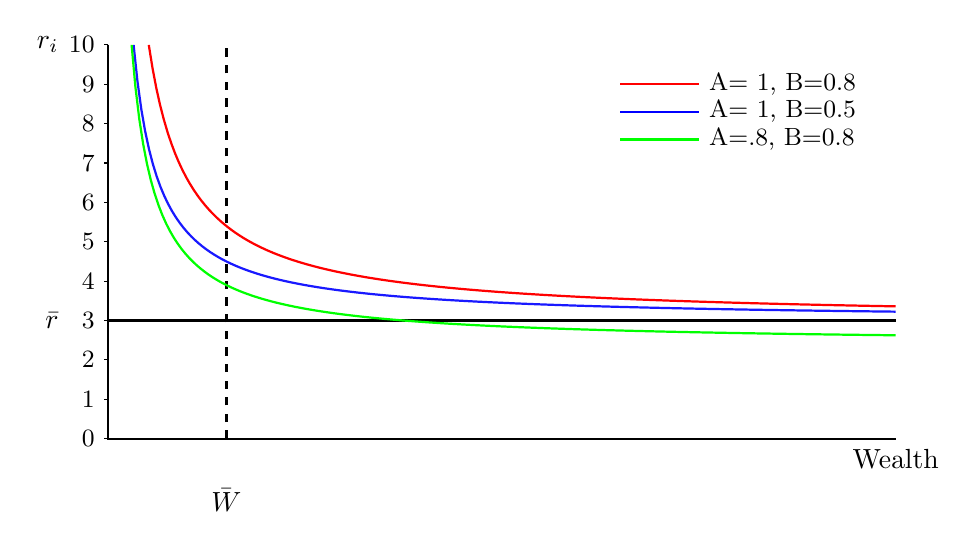
\begin{tikzpicture}[scale=.5]
%\def\bndmax{5}        %https://tex.stackexchange.com/questions/68462/filling-a-complex-region-with-tikz
%\def\bndmin{0.2}
\def \Y {10}  % height of y axis pecent
\def \W {20}  % length  of x axis
\def \Wbar {3} % jmeam wealth
\def \omega {3}
\def \A {1}  %was .5
\def \B {.5}
%Equation   \[ r_i = (A + .5 \frac{\bar{W}}{W_i})\omega\]
\def \Wmin{.63}  %This sets the lower limit fo the 
\def \Wmin{(\B*\Wbar)/(\Y/\omega-\A)} %function to keep in in bounds
	
\tikzset{func/.style={thick,color=blue!90}}	

\draw [thick] (0,\Y)node[left=.5cm]{$r_i$} -- (0,0)--(\W,0)node[below]{Wealth};  	% Axes
\draw [thick] (0,\omega)node[left=.5cm]{$\bar r$} -- (\W,\omega);  	% Axes
\draw [thick,dashed] ( \Wbar,0)node[below=.5cm]{$\bar{W}$} -- (\Wbar,\Y);  	% Axes

\foreach \yi in {0,...,\Y} \draw (0,\yi)--(-.1,\yi)node[left]{\small$\yi$};

\draw[func,domain=\Wmin:\W] plot [samples=200] (\x,{(\A+\B*\Wbar/\x)*\omega});
\def \A {.8}
\draw[func,domain=\Wmin:\W, green] plot [samples=200] (\x,{(\A+\B*\Wbar/\x)*\omega});

\def \A {1}
\def \B {.8}
\draw[func,domain=\Wmin:\W, red] plot [samples=200] (\x,{(\A+\B*\Wbar/\x)*\omega});

\draw [red,  thick](13, 9)--(15,9)node [right, black] {\small A=\ 1,\ B=0.8};
\draw [blue,  thick](13, 8.3)--(15,8.3)node [right, black] {\small A=\ 1,\ B=0.5};
\draw [green, thick](13, 7.6)--(15,7.6)node [right, black] {\small A=.8, B=0.8};
 \end{tikzpicture}
% Figure of cost of borrowing
%\caption{Hypothetical wealth-dependent borrowing cost}
%\label{Fig:BorrowingCost}
%\end{center}
%\end{figure}%

This has a number of immediate implications. First, if agents discount at their borrowing rate, wealthier agents a lower discount rate and therefore value properties more highly. 

Second, given the  common rule that mortgage payments cannot exceed some fraction of disposable income, the wealthy will be able borrow larger amounts and at lower interest rates that the less wealthy. At any distance from the centre they will be able to make a higher bid.
 
If the expected return on a property is greater than the individual cost of borrowing, it would pay any agent to borrow as much as possible and purchase properties as they become available.

\subsubsection{The rate of return on a property purchase $v$}
To explore the implication of the financialization of the urban land market we need a function to calculate the return on a unit of land that reflects the actual gradient of opportunity in financial markets. We begin with the price appreciation, $\Delta P=P_T-P_0 = (1+\dot p)P_0-P_0 $, where $\dot p$ is the rate of price appreciation over the period $T$. Rates will all be specified for the period $T$. Transaction costs, including real estate fees, take a fraction from the value of the final sale.

 The speculator invests a down payment, $D$, and gets back at time $T$ the  increased price $(1+\dot p)P_0$, plus rents, minus any costs and minus the mortgage with interest.
%footnote{We can include a use value, $U$ in place of rent for expatriate owners to represent using the property - say one month a year - when they are not renting the property and a \textbf{vacancy tax},
%$T$ at rate $t$ to affect the speculator's  decision.
 
The rate of return is the value of the gain, $V$,  over the size of the downpayment, $D$, where
\begin{equation}
V =capital\ gain - Interest\ due  	+ Rent  - operating\ cost\    
\end{equation}

The rate of return is $v = \frac{V}{D}$. 

Both the  share of the price  that can be mortgaged, $m$, and the interest rate  and $r$ may be functions of the agent's wealth. $\delta$ represents the net capital gains tax. It makes it possible to capture the capital gains kept. If it is set to one, it simplifies the equations, all is kept. Keeping the variable offers a policy variable to control the return on financial capital.

\begin{eqnarray*}
V  %	&=& capital\ gain - Interest\ due  	+ Rent  - operating\ cost\\
% 	&=& \delta P_T-D \qquad \qquad \quad - (1+\delta r)M \quad	 + R  	-C\\
% 	&=& \delta P _T \qquad-(P_0-M) \quad- (1+\delta r)M 	 + R  	-C\\
%	&=& \delta (1+\dot p)  P_0 -(P_O -M)  -(1+\delta r)mP_0  + R  -C\\
%	&=& \delta (1+\dot p)  P_0 -P_O + M \qquad -(1+\delta r)mP_0  + R -C\\
%	&=&( \delta (1+\dot p)-1)  P_0  + mP_0 \quad -(1+ \delta r)mP_0  + (\rho-\kappa)P_0\\	
%	&=& \left(  \delta (1+\dot p)-1    + m \quad - m(1+\delta r)  + (\rho-\kappa)\right)P_0\\'
%	&=& \left(  \delta (1+\dot p)-1    + m \quad - m-\delta rm  + (\rho-\kappa)\right)P_0\\
&=& \delta(P_T- (1+r)M) \qquad \qquad 	 + R  	-C   - T\\
&=& \delta((1+\dot p)  P_0- (1+r)mP_0)   + \rho P_0  	-\kappa P_0 - tP_0\\
&=&( \delta((1+\dot p)  - (1+r)m) \ + \rho   	-\kappa -t) P_0
\end{eqnarray*}

This is the  net present value of buying, and selling after one period. \textbf{It has  6 exogenous parameters}. Operating revenue and costs $ \rho -\kappa - t$ a present value. 

The rate of return is $v = \frac{V}{D}$. For expat investors, we get a \textbf{decision rule}:\begin{enumerate}
\item  if $v \geq a$ (with some private use?) with no rent,  don't bother renting. 
\item If $v(no\ rent\ and\ tax) < a\leq v(with\ rent)$,  then  rent. 
\item If $ v(with\ rent) \le a $,  then sell 
\end{enumerate}


We can, with some simplifications, write
\begin{eqnarray}
\frac{V}{D}&=&( \delta((1+\dot p)  - (1+r)m) \ + \rho   	-\kappa - t ) \frac{P_0}{D}   \nonumber\\
		&=&( \delta((1+\dot p)  - (1+r)m) \ + \rho   	-\kappa - t ) \frac{P_0}{P_0-mP_0}   \nonumber\\
		&=&\frac{ \delta(1+\dot p  - (1+r)m) \ + \rho   	-\kappa - t } {1-m} \label{Eqn:DecisionRule}
\end{eqnarray}

\subsubsection{Returns on capital are higher for wealthy investors}
\[   r^h=\frac{ \delta(1+\dot p  - (1+r)m) \ + \rho   	-\kappa - t } {1-m}    \]
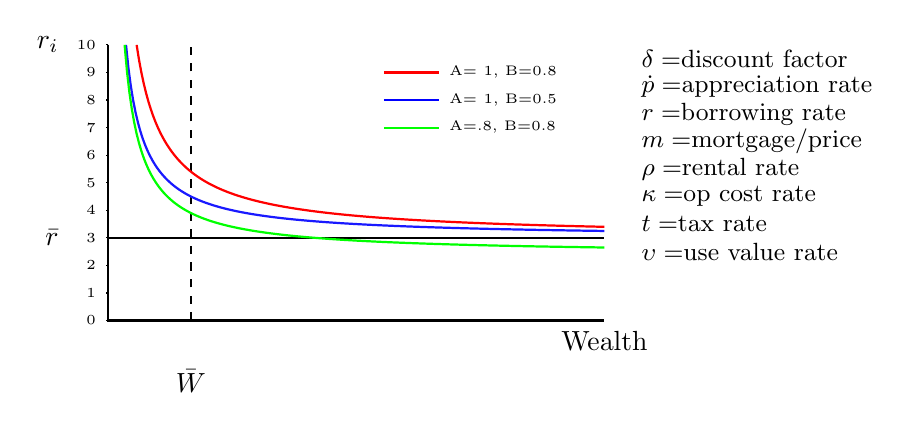
\begin{tikzpicture}[scale=.35]
%\def\bndmax{5}        %https://tex.stackexchange.com/questions/68462/filling-a-complex-region-with-tikz
%\def\bndmin{0.2}
\def \Y {10}  % height of y axis percent
\def \W {18}  % length  of x axis
\def \Wbar {3} % j mean wealth
\def \omega {3}
\def \A {1}  %was .5
\def \B {.5}
%Equation   \[ r_i = (A + .5 \frac{\bar{W}}{W_i})\omega\]
\def \Wmin{.63}  %This sets the lower limit fo the 
\def \Wmin{(\B*\Wbar)/(\Y/\omega-\A)} %function to keep in in bounds
	
\tikzset{func/.style={thick,color=blue!90}}	

\draw [thick] (0,\Y)node[left=.5cm]{$r_i$} -- (0,0)--(\W,0)node[below]{Wealth};  	% Axes
\draw [thick] (0,\omega)node[left=.5cm]{$\bar r$} -- (\W,\omega);  	% Axes
\draw [thick,dashed] ( \Wbar,0)node[below=.5cm]{$\bar{W}$} -- (\Wbar,\Y);  	% Axes

\foreach \yi in {0,...,\Y} \draw (0,\yi)--(-.1,\yi)node[left]{\tiny$\yi$};

\draw[func,domain=\Wmin:\W] plot [samples=200] (\x,{(\A+\B*\Wbar/\x)*\omega});
\def \A {.8}
\draw[func,domain=\Wmin:\W, green] plot [samples=200] (\x,{(\A+\B*\Wbar/\x)*\omega});

\def \A {1}
\def \B {.8}
\draw[func,domain=\Wmin:\W, red] plot [samples=200] (\x,{(\A+\B*\Wbar/\x)*\omega});

\draw [red,  thick](10, 9)--(12,9)node [right, black] {\tiny A=\ 1,\ B=0.8};
\draw [blue,  thick](10, 8)--(12,8)node [right, black] {\tiny A=\ 1,\ B=0.5};
\draw [green, thick](10, 7)--(12,7)node [right, black] {\tiny A=.8, B=0.8};

\def \W {19}  % length  of x axis
\node[right] at (\W,9.5){\small$\delta=$discount factor};
\node[right] at (\W,8.5){\small$\dot p=$appreciation rate};
\node[right] at (\W,7.5){\small$r=$borrowing rate};
\node[right] at (\W,6.5){\small$m=$mortgage/price};
\node[right] at (\W,5.5){\small$\rho=$rental  rate};
\node[right] at (\W,4.5){\small$\kappa=$op cost rate};
\node[right] at (\W,3.5){\small$t=$tax rate};
\node[right] at (\W,2.5){\small$\upsilon=$use value rate};
 \end{tikzpicture}


% \chapter{Future Work}

Very Rough.
%TODO Diagram with colours to illustrate implemented, partially implemented and unimplemented. Show the structure of the model and potential extension.

%different equilibrium concept. --> tractability of a mechanical vs statistical equilibrium
%explain it's relation with other approaches. Link with viability too

\section{A Possible Typology of Models and Experiments}

While there  are very many variations on the basic urban model and many potential experiments with each model there are only a few of immediate interest if the goal is to text the ``resilience'' of equilibria.

These models may exhibit irreversibilies in variables such as distribution, homelessness, city form, and class structure. 


The  basic strategy for examining the system resilience is to shock a model (experiment) and then see if diagnostic variables recover. (This needs more precise expression.)


The first task is to select a subset of models an experiments that are of particular interests with respect to .

The second is to construct  a model that allows those case to be examined. Ideally the model would be easily adapted to other experiments.

The following is a an attempt to develop a typology with a clear  progressive structure.

Feedback - wealth  allows  upgrading. This advantages the rich. Maybe this 



\begin{enumerate}
\item \textbf{A: The Basic Model}

As used as the basis of the analytic model in this thesis, the workhorse of urban economics is the circular city model. Some feature of the central place generates rents. It may be that it is the only employment centre. It may be economies of scale to a single activity or synergies arising from various externalities.

If population exceeds the number of properties there are three margins to consider
	\begin{enumerate}
		\item The land supply can increase. There may be a conversion cost
		\item The land per-capita may decrease. This is not simple in a city with land-use regulations, zoning, and fixed capital in homes. A conversion process has to be defined
		\item A homeless population can emerge. 
	\end{enumerate}
	
\item \textbf{Y: The Basic Model with Income Differences}
This will result in segregation by neighbourhood depending on income. 

Income can be purely earning, which requires a distribution of $w$ across agents. Income  might include investment income, which  a private rate of return and a distribution of assets across agents. \footnote{A more subtle model could allow individual wages to be linked to the agglomeration of other workers - say engineers. we can imagine a city that has centres of agglomeration by profession or by complementarity. Depending on the production function, this should emerge endogenously.}
\footnote{Sufficient investment income could lead individuals to locate in cheap properties at the edge of the city.  Income might also be invested in property affecting the quality of a unit. This would require incorporating unit quality in the attribute list for each property, and introducing a quality preference  in the attribute s of residents.}


\item \textbf{L: The Basic Model with Locational Preferences}
This will result in segregation by neighbourhood depending on preferences.

One version would be include distance to the edge of the city as an amenity in the utility function. Another would be to locate amenities within the city. These would lead to higher prices near amenities.

A natural variant would be to have earning depend on location. If there were several locations  a polycentric city would emerge.

\item \textbf{T: The Basic Model with Varied Transportation Cost }
This will result in segregation by neighbourhood depending on income and Transportation costs. Experiments include cars for the rich and  transit. 

Diagnostics include change in total transportation cost and differential welfare effects.


\item \textbf{R: The Basic Model with a Rent-own choice}
This may result in the emergence of classes. Agents must have the capacity to borrow to purchase. Attributes of the agents and must now include  net assets,  an available interest rate, and a permissible mortgage.

We imagine a banker setting the mortgage rates and size. This can be done at the beginning of each period for each agent. 

With no income differentia we expect equal utilities

\item \textbf{YR: The Basic Model with Earnings (Y) Differences and a rent-own choice}
This model is very likely to generate diverging classes as income differentials permit some to capture land rents from others. This is highly likely if borrowing costs decline with income and asset ownership.

\item \textbf{L: The Basic Model with Variable lot size}
This is achieved by making lot size a choice variable for households, in which case we will get a tradeoff between transportation cost and lot size and distance. Results for this model are known. Density  falls with distance from the centre. 

\item \textbf{YL: The Basic Model with Earnings (Y) Differences and Variable lot size}
The wealthy choose larger homes and lots farther form the centre

\item \textbf{S: The Basic Model with constant lot size and variable density}
This is achieved by allowing stacking of housing units. Results for this model are not known. This introduces a step change in housing form, and emphasizes unit size.

This model should produce some interesting spatial patterns, especially if couples with the possibility of secondary central places.

\item \textbf{YS: The Basic Model with Earnings (Y) Differences, constant lot size and variable density}

This model should produce some interesting spatial patterns, especially if couples with the possibility of secondary central places.


\item \textbf{IR: The Basic Model with outside investors and rent-own}

\item \textbf{IYR: The Basic Model with outside investors, Earnings differentials and Rent-own choice} This model is of interest if borrowing costs decline with income and asset ownership.
\end{enumerate}


\subsection{Experiments}
There are various experiments of interest. You will have to pick key ones. It is not necessary to do all of them in every model. 

	\begin{enumerate}
		\item increase population
		\item increase wage\
		\item add hard boundary (limit land)
		\item Introduce differential incomes
		\item Introduce differential access to capital
	\end{enumerate}

%\newcommand{\cred}{\cellcolor{red!30}}
\begin{table}[htp]
\caption{Potential experiments: \textbf{Pick some}}
\begin{center}
\begin{tabular}{|c|c|c|c|c|c|}\hline

  &\multicolumn{5}{c|} {experiments}\\ \cline{2-6}
Model   & 1 & 2  & 4 & 4  & \\ \hline
 A         &    &     &   &   &   \\
 Y         &    &   &   &    &   \\
 T         &    &    &    &    &   \\
 R         & etc &  &  &  & \\
 L         &  &  &  &  & \\
 S         &  &  &  &  & \\
 I          &  &  &  &  & \\
 YR       &  &  &  &  & \\
 IR        &  &  &  &  & \\
  IYR     &  &  &  &  & \\\hline
\end{tabular}
\end{center}
\label{default}
\end{table}%

%\newcommand{\cred}{\cellcolor{red!30}}
%\begin{table}[htp]
%\caption{Potential experiments: \textbf{Pick some}}
%\begin{center}
%\begin{tabular}{|c|c|c|c|c|c|}\hline
%
%  &\multicolumn{5}{c|} {experiments}\\ \cline{2-6}
%Model  &1 &2  & 4 &4  & \\ \hline
% A& \cred& \cred  &  \cred & \cred  & \cred  \\
% Y& \cred   & \cred   & \cred   &\cred    &\cred   \\
% T & \cred   & \cred   & \cred   &\cred    &\cred   \\
% R & etc &  &  &  & \\
% L &  &  &  &  & \\
% S&  &  &  &  & \\
% I &  &  &  &  & \\
% YR &  &  &  &  & \\
% IR &  &  &  &  & \\
%  IYR&  &  &  &  & \\\hline
%\end{tabular}
%\end{center}
%\label{default}
%\end{table}%


\subsection{Development}
\label{Sec:Development}

In addition to rent, there is development. Rent is distinct from the process of densification. Developers do work to to create additional housing supply, which can create value for those seeking to live near the centre, by increasing the supply of housing per unit of land. The value created by developers can be claimed by land owners.

 Research on scaling of the skyline gives a basis for approximating rents. 
The process of development introduces non linear dynamics into the the supply. - matching problem.
It is a political process where cities can direct and limit density to particular regions. 
Developers often also own the land they develop, which means they could claim the rents.



% \addcontentsline{toc}{chapter}{APPENDICES}
\chapter*{Appendix: Notation}
%\newpage

%omega is the slope of the budget life, a calculation variable, the ratio of capital costs to labour costs.

\begin{center}
\begin{longtable}{lp{10cm}}
\caption{Notation}\\\hline
		&\textbf{Productivity}\\ \hline
$K$  &  Capital\\
$n_i$  &  Number of workers employed by firm $i$\\
$n=\sum_i n_i$  &  Labour (number of workers)\\
%$f$  &  Number of firms\\
%$n =f n_i$  &  Aggregate labour \\
$\Lambda(n)$  &  Labour-augmenting agglomeration effect \\
% $n^\gamma$ & The labour-augmenting agglomeration effect,  modelled as an expontial function of the number of people \\
$\Lambda(n)n$  &  Effective labour \\
%$\Lambda'=\die{\Lambda(n)}{n} $ & Derivative of the labour-augmenting agglomeration effect\\
$\alpha$  &  Elasticity of output with respect to capital\\
$\beta$  &  Elasticity of output with respect to effective labour\\
$\gamma$  &  Elasticity of $\Lambda(n)$, labour-augmenting agglomeration\\
$Y=K^{\alpha }(\Lambda(n)n)^{\beta }$  &  Aggregate output of all firms in the city\\
$Y_i=K_i^{\alpha }(\Lambda(n)n_i)^{\beta }$  &  Urban firm $i$'s output\\
$\die{Y_i}{K_i}	=\alpha \frac{1}{K_i} Y_i $  & Marginal product of capital for firm $i$
\\
$\die{Y_i}{n_i}	=  \beta\frac{1}{n_i} Y_i $  &  
Marginal product of labour for firm $i$\\
$\die{Y}{n}=\beta\frac{1}{n_i} Y_i  \left( 1+ \frac{n\Lambda'}{\Lambda} \right) $  &  Social marginal product of labour\\
$\eta=\frac{n\Lambda'}{\Lambda}$  &   Marginal agglomeration effect on aggregate labour productivity\\
\hline
	&\textbf{Amenity}\\ \hline
$A(d, n)$   &  Agglomeration amenity\\
\hline
		& \textbf{Prices}\\ \hline
$\psi$  &  Rural wage\\
$\psi$  &  Per-period cost of a unit of productive capital\\
$w$  &  Urban wage premium\\
$\psi + w$  &  Urban wage\\
$\Omega=\frac{w+\psi}{\psi}$  &  Ratio of the urban wage to the  cost of capital\\
\hline
		&\textbf{Spatial structure in the circular city}\\ \hline		
$d$  &  Distance of a residence from the centre of the city\\
$\tau$  &  Linear transportation cost per unit distance\\
$c^{max} = w/\tau$  &  Maximum distance commuters will travel% for wage $w$
\\
$s$ & Lot size\\
$U$  &  Worker utility, a function of location and prices\\
$U^{urban}=U^{rural} $  &   Migration equilibrium assumption\\
\hline
		& \textbf{Labour market}\\ \hline
$L= \frac{\pi}{s}(\frac{w}{\tau})^2 = n$  &  
Labour supply, the number of workers, which equals the number of lots in the standard circular city model since workers live on identical individual lots\\
\end{longtable}  \end{center}



\chapter*{Appendix: Excess Return on Urban Capital}\label{Sec:ExcessProfit}

% At this point we may consider a contradiction. 
There is a problem. How to calculate how firms will respond?
We can calculate the labour-capital ratio and aggregate output based on the assumption that firms assume that the agglomeration effect in their production function is fixed. This assumption is reasonable. It seems likely that the agglomeration effect of adding a worker would be difficult to attribute to a new worker: it would be a lagged, unevenly distributed effect, and would appear exogenous\footnote{It is possible to interpret in other ways. Perhaps firms linearly extrapolate rewards. See xx for a review of approaches to modelling firm behaviour.}. 
If it is reasonable to assume that firms would not take the agglomeration term into account and the effect is thus not be compensated. This gives *** TODO labour-capital ratio and aggregate output
%The effect of adding a worker $Y_i \frac{\Lambda'}{\Lambda}$
%Assuming firms do not take the adjustment of the agglomeration term into account. 


Assuming firms take the wage as parametric and hire until the private myopic marginal product falls to the observed wage, % *** What does parametric mean here?

		\[  \beta\frac{1}{n_i} Y_i =    w+\phi , \]
%implying firms will hire fewer than the optimal number of workers.

Since urban firms pay each worker the private marginal product but gain from each worker the effective marginal product,   plus a share $n_i/n$ off the extra social marginal product, $\eta=\frac{n\Lambda'}{\Lambda}$.  There is a potential  inefficiency that arises from a failure to take into account the externality. 
%$The answer may depend on whether there is firm entry   !!!!

% *** WHAT IS THE UNDOING EFFECT? WHAT DO WE MEAN BY SYNCHRONIZED
%Will this information lead to undoing the effect?  - I don't think so - if hiring is NOT synchronized, breaking the link with own hiring future productivity would be tied only to expected population growth which will appear exogenous.
%

\begin{align} 
\die{Y}{n}=&\beta K^{\alpha }(\Lambda(n)n)^{\beta-1 }(T'n+T )  \nonumber \\
		=&\beta  \frac{K^{\alpha} (\Lambda(n)n)^{\beta}}  {\Lambda(n)n} (\Lambda'n+T)  \nonumber \\
		=&\beta  \frac{K^{\alpha} (T(n)n)^{\beta}}  {\Lambda(n)n} (\Lambda'n+\Lambda)  \nonumber \\
	Y_n	=&\beta \left( \frac{1}{n}+ \frac{\Lambda'}{\Lambda(n)} \right)	Y
\end{align}

Assuming all firms behave the same way, the social marginal product, taking into account the agglomeration effect is  

\[ \frac{n}{n_i} \die{Y_i}{n_i} \]


 marginal product of capital
\begin{align}
Y=&K^{\alpha }(\Lambda(n)n)^{\beta}   \nonumber  \\
\die{Y}{K}=&\alpha K^{1-\alpha }(\Lambda(n)n)^{\beta }  \nonumber \\
		=&\alpha \frac{K^{\alpha}(\Lambda(n)n)^{\beta }}{K}  \nonumber \\
	Y_K	=&\alpha\frac{1}{K} Y  \label{EQ:mpk}		
\end{align}
The aggregate marginal product of capital for the firm does not differ from the private marginal product of capital.


\hrule 

The marginal product of labour, however,  is complicated by the presence of the  agglomeration effect , $\Lambda(\sum n_j)$:
\begin{eqnarray} \die{Y_i}{n_i} &=   K_i^\alpha \left(  \beta\Lambda n_i^{\beta-1}  + n_i^{\beta}\Lambda'  \right)  \nonumber\\
&=   \beta\frac{1}{n_i} Y_i   +  Y_i \frac{\Lambda'}{\Lambda}  \nonumber\\
&=   Y_i  \left[  \beta\frac{1}{n_i}  + \frac{\Lambda' }{\Lambda} \right]   \label{Eqn:MPL}
\end{eqnarray}
The first term in the square bracket in Equation~\ref{Eqn:MPL} might be termed the \textbf{private myopic marginal product}. It is the addition to output directly attributable to an additional worker. This myopic MPL is smaller than the actual marginal product for the firm.  
The second term in the bracket   is the marginal agglomeration effect. It captures the effect on firm-wide labour productivity -- an increase in effective labour --   that results from adding a worker. We can expect this to be very small.\footnote{Using the specification in Footnote~\ref{Fn:PSI}, $Lambda(n)=n^\psi$, it would be $\frac{\psi}{n}$. If f $\psi=0.1$ and $n=250,000$ the number is $\frac{\Lambda' }{\Lambda} =4\times 10^{-7}$.}% REVIEW THIS 
% REVIEW THIS TOO
%\footnote{Firm size matters. 
%A monopoly employer would take into account the marginal agglomeration effect. 
%A firm that employed a large enough fraction of the urban workforce to notice agglomeration effects, say $\frac{1}{n}<k<1$, would enjoy that fraction of the external effect and set the wage at  
%\[w_k =  \beta\left( \frac{1}{n}+ \frac{k\Lambda'}{\Lambda(n)} \right)	Y\].} 

\subsubsection*{The Size of the Excess Return}
The surplus return to a firm's capital from adding one worker to the firm is the value of the marginal product of the increase in effective labour net of the additional wage payment.  Since workers are paid their myopic marginal product, the unexpected  excess return (ER) is 
\begin{eqnarray}
%\die{Y_{i}^a}{n_i} -(w +\psi) =& \frac{\beta}{n_i}  Y_i  \left[  \beta\frac{1}{n_i}  \\%+  \frac{\Lambda' }{\Lambda} Y_i    \beta\frac{1}{n_i} } \\
				ER	&=&   Y_i  \left[  \beta\frac{1}{n_i}  +  \frac{\Lambda' }{\Lambda} \right]   -Y_i  \left[  \beta\frac{1}{n_i} \right]\\
					&=&  Y_i   \frac{\Lambda' }{\Lambda}\\
\end{eqnarray}	
%The aggregate excess is simply $Y \frac{\Lambda' }{\Lambda}>0$. 
As a result, the urban economy should experience both firm expansion and firm entry. %This may be consistent with empirical research by Brown and Rigby (2013) showing that smaller and younger firms experience stronger productivity gains stemming from the localized pooling of workers with skills that match their needs and from knowledge spillovers than do larger firms. 

%\[w^t \Rightarrow n^t, k^t \Rightarrow  \pi^t>0  \Rightarrow w^{t+1} >w^t,  \#f^{t+1}> \#f^t \]
%A unit of urban capital therefor earns its own marginal product, $Y_K= \alpha Y/K$ 

The rate of excess return is the excess return divided by the size of the firm's capital stock, $K_i$. We can find the aggregate capital stock on the assumption firms maximize profits, which leads them to (myopically) set 


\begin{eqnarray}
\frac{ \Large{\die{Y_i}{n_i} }} { \Large \die{Y_i}{K_i} }&=\frac{ w+\psi }{ r }\nonumber \\
%	\frac{\cfrac{\partial Y _i}{\partial K_i}}{\partial K_i}=&\\%
%\frac{\frac{\beta}{n_i} Y_i }{ \frac{\alpha}{K_i} Y_i}&=\Omega\\%\frac{w+\psi}{\psi}\\
\frac{\beta}{\alpha}\frac{K_i}{n_i} &=\Omega \nonumber
\end{eqnarray}
so we can express the individual firm capital capital stock desired 
\begin{equation}
K_i =\frac{\alpha}{\beta}\Omega n_i\\
\end{equation}
Which in increasing in $n_i$.
 
%%%%%%%%%%%%%%%%%%%%%%%%%%%%%%%%%
%\textbf{\color{green}]Hidden section: the rate of excess return is always positive. }
so the rate of excess return is 
\begin{eqnarray}
\frac{ER}{K_i} &=\frac{Y_i   \frac{\Lambda' }{\Lambda}}  {\frac{\alpha}{\beta}\Omega n_i }   \nonumber\\
&=\frac{ 1}  {\alpha\Omega }\frac{\Lambda' }{\Lambda}\frac{\beta}{n_i }Y_i    \nonumber \\
&=\frac{ r}  {\alpha(w+\psi) }\frac{\Lambda' }{\Lambda}\frac{\beta}{n_i }Y_i 
\end{eqnarray}
which is always positive. %The last two terms in the expression are the myopic marginal product of labour.

 %\textbf{\color{green}Hidden section: wage bill is increasing with the cube of the wage}
% USEFUL   Notice that the wage bill is increasing with the cube of the wage, which could  be a powerful driver of demand for services and commercial and hence for urban commercial development. We will reexamine this observation below.

%We assume that demand for the urban product is perfectly elastic and the price per unit is 1. 




%
%We know the population, $n$, is simply the area of the city divided by the lot size, and the area is a function of the wage premium $w$.   The wage bill is 
% \[W	= (\psi + w)\frac{\pi }{s}  \left(\frac{w}{\tau}\right)^2\]
%
%
%
%With full employment, aggregate   demand for labour $\sum_i n_i,$  is equal to supply from  Equation~\ref{supply}, which gives us a way to calculate the aggregate capital desired
%
%\begin{eqnarray}
%\mathsmaller{\sum_i} K_i &=\frac{\alpha}{\beta}\Omega \sum_i n_i,\\ %note I have added package relsize 
%K &=\frac{\alpha}{\beta}\Omega n\\
% &=\frac{\alpha}{\beta}\Omega L,
%\end{eqnarray}

%
%Firm $i$'s output is 
%\begin{eqnarray} 
%Y_i	=&   \left( \frac{\alpha}{\beta}\Omega n_i \right)^\alpha  \left(\Lambda(n) n_i \right)^\beta  \nonumber\\
%	=& \left( \frac{\alpha}{\beta}\Omega\right)^\alpha n_i ^\alpha \Lambda(n)^\beta n_i ^\beta \nonumber \\
%	=& \left( \frac{\alpha}{\beta}\Omega\right)^\alpha \Lambda(n)^\beta n_i ^{\alpha + \beta}
%\end{eqnarray} 
%
%Firm profit is then
%
%\begin{eqnarray} 
% \Pi 	=&p \left( \frac{\alpha}{\beta}\Omega\right)^\alpha \Lambda(n)^\beta n_i ^{\alpha + \beta}
% -\Omega n_i -\psi \frac{\alpha}{\beta}\Omega n_i    \nonumber\\
%	=& p\left( \frac{\alpha}{\beta}\Omega\right)^\alpha \Lambda(n)^\beta n_i ^{\alpha + \beta} -\left(\Omega + \psi \frac{\alpha}{\beta}\Omega\right) n_i  \\
%	=& p\left( \frac{\alpha}{\beta}\Omega\right)^\alpha \Lambda(n)^\beta n_i ^{\alpha + \beta} -\left(1 + \psi \frac{\alpha}{\beta}\right) \Omega n_i  
%\end{eqnarray} 



% \textbf{\color{green}Hidden section: crosspartial  $\die{\frac{\alpha Y}{K}}{n}$}
%\begin{align} 
%\die{\frac{\alpha Y}{K}}{n} 	=&	\frac{\alpha}{K} \die{Y}{n}  \nonumber  \\
%					=&	\frac{\alpha}{K} \beta\left( \frac{1}{n}+ \frac{\Lambda'}{\Lambda(n)} \right)	Y \nonumber \\
%					=&\alpha(1-\alpha)\frac{K^{\alpha}(A(n)n)^{1-\alpha }  {KA(n)n)}(A'n+A) \nonumber \\
%					=&\alpha\beta\frac{Y}{K}\left( \frac{1}{n}+ \frac{\Lambda'}{\Lambda(n)} \right) \nonumber \\
%\end{align}

\subsubsection*{Method 2: Zero Conjectural Variation}

? Another way to consider how firms will respond is to assume they xyz- 0 conjectural variation. This is different from the above in that xyz....

Even taking into account firm-wide labor productivity gains, the private marginal product of labour is likely to be computed on the assumption that other firms do not expand  their workforce. This could be call the `zero conjectural variation' (0CV) case. If all firms  were expected to respond to the same signal the same way (1CV), the agglomeration effect  would be multiplied by the number of firms, $\frac{n }{n_i}$ . The marginal agglomeration effect for firm $i$ is then $\frac{n }{n_i}\frac{\Lambda' }{\Lambda}Y_i =\frac{\Lambda' }{\Lambda}Y$. 

Since the increase in $\Lambda$ affects all firms, the  social marginal product of all firms expanding their  workforces by one worker as $i$ does must be multiplied again by the number of firms. The value of the agglomeration effect  becomes large with a large number of firms. %(agents?) 


%\begin{figure}[tb]
%\begin{center}
%\input{SA_AmenityFigure.tex}
%\caption{Incorporating an consumption amenity}
%\label{default}
%\end{center}
%\end{figure}


\begin{eqnarray}
\die{Y}{n_i}=&   \beta\frac{1}{n_i}Y_i    + \frac{\Lambda' }{\Lambda}\sum_j Y_j\frac{n }{n_i} \\
%
		=&   \beta\frac{1}{n_i}Y_i    + \frac{\Lambda' }{\Lambda}Y\\
\end{eqnarray}		
 where $\frac{n }{n_i}$ is the number of firms. 




\subsubsection*{Underfunded Public Amenity}

The firm's assumption is incorrect however: the agglomeration effect is not fixed. It increases with the growing urban population, as more firms hire and attract more people. The firm thus experiences greater productivity growth than expected.% because it does not account for the agglomeration effects. 
Which means the firm's realized output, revenue, and profit are higher than expected. % for each firm, is higher than planned output, as are revenue and profits. %If urban firms capturing 
%If firms choose labour and capital to maximize profit given assumptions about the production function, and then enjoy unexpected high productivity productivity increases, which implies that the firm will find realized profit higher than expected  and, presumably, adjust its estimate of the marginal product of labour upward, and therefore demand more labour.

This excess return has the potential to drive firm expansion, firm entry, and the continual growth of the urban economy. %city. The result should be continuous growth of the urban economy. %(Will that growth converge or will it be unbounded?)

% because of the agglomeration effect, effective labour productivity will be greater than expected.

%We have calculated the labour-capital ratio and aggregate output based on the assumption that firms incorrectly assume that the agglomeration effect in their  production function is fixed. %This must hold in an equilibrium. 

In both scenarios agglomeration generates a public good that is underfunded privately.
The agglomeration effect is a public good in which individual firms under-invest. This raises a potential policy challenge. % that we leave for others.

%? a differential equation or difference equation in which $w_t \rightarrow n_{t+1} \rightarrow w_{t+1}$. How to write this? Do we  need to?)

These observations about a rising the rate of return on urban capital raise a set of very interesting issues.   
\begin{enumerate}
\item The effect of increasing the urban workforce is to increase the marginal products of  both capital and labour throughout the urban economy. This premium on production in cities is positive when $\Lambda'$ is greater than zero.
 \item  As long as $\Lambda'>0$ cities will  grow, potentially leading to the ``catastrophic agglomeration''  that has been noted in other models.  (\cite{FujitaKrugmanVenables, BaldwinMartin, Krugman1991, Gurwitz2019}).  City size could be bounded, in which case the city system would grow by increasing the number of cities. This appears to depend on the model features and parameters. 
 \item Even in competitive markets, until the wage rises, capital is capturing all of the socially produced benefit of agglomeration. (We will see below that the rest is captured by landowners.)
%\item it brings into question the standard assumption of an equilibrium  rate of return on capital.  
%\item It appears firms will capture all of the socially produced marginal product of agglomeration.

\item Cites will draw investment away from rural and remote areas.

\item Cites will draw labour away from rural and remote areas.
\end{enumerate}

These are features of the economy we observe.

\chapter*{Appendix: Amenity, Income, and Land Rent}

%Non monetary income well established for business literature, now extend to the city.
%Rent in the city can come from two places:
%1. generated through production function
%2. rent generated through some locally produced amenity. 
%There are papers that look at the Henry George rule for each case. The standard examination works on investment in amenity rather than production--public investment in either productivity or amenity.

If a city offers amenities, in addition to employment opportunities, their value appears in the rent profile. A simple way to incorporate agglomeration amenities is to include what might be called a `utility premium' for urban dwellers as non-monetary location income $A(d,n)$ where $A$ is amenity also located at the centre initially for convenience, $d$ is the distance from the amenity, and $n$ is the urban population. 

Amenity declines moving away from the centre and increases with the population so $\die{A}{d}\leq 0,\die{A}{n}\geq 0$. The logic for all kinds of urban amenities, from hospitals, lessons and research institutes, to clubs,  is similar to that for productive agglomeration. For example, with a hospital, in an urban centre, more people share the resource but a larger city can invest more so the hospital can purchase more equipment and offer more treatments. %Costs per person go down since it is shared. 
Specialty services, that might largely empty in a small hospital, get fuller utilization so the cost of operation can be lower. This allows more and cheaper services. This is compounded by the specialization of labour and the network of experts available nearby. There are transportation benefits if buses run to the centre and utilities scale sub linearly.

These amenities offer value that feeds directly into the rent profile. Those with the means are willing to pay more to live near amenities, 


 

Those which are available only to those very close. Some are free, some require fees. 


Amenities will affect peoples behaviour and be reflected in the rent profile. No amenities, it will be the wage, rental cost and transportation.
Throw in amenities. 



If $A=0$ %and $T=td$, \label{Eqn:U} 
 this model produces the standard result in the Alonzo model: land rent declines linearly with distance. 
 
If $A(0)>0$, willingness to pay and therefore the competitive rent profile is higher than the if there is only a wage premium.  
Migrants to the city will be a self-selected subset of all workers for whom the urban amenity is a substitute for something in the standard bundle purchased out or $\psi$. 
The rent profile is  
\begin{equation}
Rent(d)  =  w  + A(d) - \tau(d)	
\label{Eqn:Rent-at-d}\end{equation}
If we solve $w+A(d)-\tau d=0$ for $d$, we get the maximum  distance at which living near the city offers an advantage, $d^{max}$. 
For example, if  $A(d)=a_0 - b*d$ and transportation costs are  linear function as above

\begin{eqnarray}
w+ a_0 - b*d^{max} - \tau*d^{max}  	&=0		\nonumber \\
w+a_0 - (b+\tau)d^{max}  	&=0			\nonumber \\
d^{max}				&= \frac{w+a_0}{b+\tau}
\end{eqnarray}
For the case of a circular city, the area within this radius is $\pi \left(\frac{w+a_0}{b+t}\right)^2$. 
If the lot size is $s$ as before, we have the aggregate population for the city. 
 \[P= \frac{\pi}{s}  \left(\frac{w+a_0}{b+\tau}\right)^2,\]
Which is larger than the number of commuters if $a_0/b>w/\tau$% Commuters will only travel to work if the wage premium minus travel costs is positive. 
 To get total land rent with a consumption amenity, we integrate:

\begin{eqnarray}   %Total rent
R&=&  \int_0^{c^{max}} ( w-\tau d) \frac{2\pi d}{s}dd 	
	+ 	\int_0^{d^{max}} (a_0- bd	) \frac{2\pi d}{s}dd 	\nonumber \\	
	&=& \frac{\pi}{3}\left(\frac{w}{\tau}\right)^2w
	+	\frac{\pi}{3}\left(\frac{A_0}{b}\right)^2w
%	\nonumber \\
\end{eqnarray}




%The first term yields
%\begin{eqnarray}
%	&=&\frac{2\pi }{s} \int_0^{d^{max}} \left( ( w+a_0)d - (b+t)d^2\right)  dd  	 \nonumber \\
%	&=& \frac{2\pi }{s} \left[ \frac{1}{2}(w+a_0)(d^{max})^2 - \frac{1}{3}(b+t)(d^{max})^3\right]  
%\nonumber \\
%	&=& \frac{2\pi }{s} \left[ \frac{1}{2}(w+a_0) - \frac{1}{3}(b+t)d^{max}\right](d^{max})^2  \end{eqnarray}
%					&= &   2\pi\left[(w+a_0)d^{max} - \frac{1}{2}(b+t)d^{max}d^{max}\right]\\
%					&=&    2\pi\left[(w+a_0)d^{max} - \frac{1}{2}(w+a_0)d^{max}\right]\\
\begin{eqnarray}
					&= &  2\pi\frac{1}{2}(w+a_0)d^{max}\\
					&= &  \pi(w+a_0)d^{max}
\end{eqnarray}

\begin{eqnarray}Rent	&=&  \int_0^{d^{max}}( w+a_0 - (b+t)d) dd\\  % linear model
					&=&  (w+a_0)d^{max} - \frac{1}{2}(b+t)d^{max^2} \\
					&= &  (w+a_0)d^{max} - \frac{1}{2}(b+t)d^{max}d^{max}\\
					&=&   (w+a_0)d^{max} - \frac{1}{2}(w+a_0)d^{max}\\
					&= &  \frac{1}{2}(w+a_0)d^{max}
\end{eqnarray}

WHAT DOES THIS MEAN?
NOTE: a simpler version  with a two-sided linear city $\kappa$ lots wide and  one unit in depth is more ``intuitive'':
\[R	= \frac{\kappa}{2} \left[\frac{w^2}{\tau} +  \frac{a_0^2}{b}\right] \]
and the wage bill is 
\[W	=2 \kappa \frac{w^2}{\tau} \]
In this model, land rent absorbs roughly half of the aggregate wage premium,  falling to exactly half as the amenity goes to zero. 
The rest of the wage premium is spent on transportation. 
The presence of amenities in general increases the aggregate urban rent.

\chapter*{Appendix: A More Detailed Discussion of Financialized Returns}

To explore the implications  of the financialization of  the urban land market we need a function to calculate the return on a unit of land, h, which that reflects the actual gradient of opportunity in financial markets. We begin with the price appreciation, $\Delta P=P_T-P_0$. Transaction costs including real estate fees, take a fraction from the value of the final sale, leaving $\phi^sP_Th$ where $\phi^s<1$ is the share remaining for the seller. Moving costs, legal fees and land registration costs add to the price of purchase, so that the full cost of purchase is $\phi^bP_0h$, where $\phi^b>1$

%\input{SA_SpeculativeMotive.tex}
%%%%%%%%  VVVVVVVVVVVVVVVVVVVVVVV   This section May 18 to cut?  V

The net gain from appreciation with transaction costs is something like \[G^N=\phi^s P_T-\delta^T\phi^b P_0=P_0(\phi^s \frac{P_T}{P_0}-\delta^T\phi^b)\]%=P_0\psi(T)\]
where $\delta^T=\frac{1}{(1+r_i)^T}$ is the discount factor for $T$ periods. The expression $(\phi^s \frac{P_T}{P_0}-\delta^T\phi^b)=C^T$ summarizes transaction costs. $\phi^s$ and $\phi^b$ represent  fixed costs that  encourage longer ownership terms, decrease mobility and make the use of the housing stock less efficient. 

If  owners take on the maximum mortgage, $M=mP_0h$ and pay interest at rate $r_i$ %we can set the  un-discounted carrying cost of ownership is simply\footnote{
and do not pay down the mortgage, the value of the infinite sum of payments $ r_iP_0$  minus the discounted long tail of payments after T is 
\[C^C= r_iM\left(\frac{1}{r_i} - \frac{1}{r_i(1+r_i)^T}\right)= mP_0\left(1- \frac{1}{(1+r_i)^T}\right) \]%=\Gamma(r,T)\]
%\[C^O= rTP_0\]$
The required downpayment is $D=(1-m)P_0$. The buyer must forego a return of $r_i^d$ and will generally encounter some transaction cost $\phi^D$ as well. As a fraction of downpayment this is  $\phi^d=\frac{\phi^D}{(1-m)P_0}$.   so this amounts to

 \[C^D=  r_i^d(1-m)P_0\left(1- \frac{1}{(1+r_i)^T}  \right)  + \phi^D  \]

The return on the investment net of carrying costs and downpayment is 

\[R=G^N-C^C- C^D  \]
Writing $\frac{P_T}{P_0}= 1+r^p$, where $r^p$ is the compounding rate of growth of housing prices over the period $0-T$,  
%&=&P_0h\left(C^T-\right)\\
\begin{eqnarray}
%R&=&P_0\left[\left(  \phi^s (1+r^p) - \delta^T\phi^b\right)  -  m\left(1- \delta^T\right)  \right]  %add D here
%- r_i^d(1-m)P_0\left(1- \delta^T\right)   + \phi^D \nonumber \\
%%  simplify last term
%&=&P_0\left[\left(\phi^s  (1+r^p) - \delta^T\phi^b\right)  -  m\left(1- \delta^T\right) \right]  %add D here
%- P_0r_i^d\left(1-m) (1-\delta^T)\right )  + \phi^D   \nonumber \\
%%  combine terms
%&=&P_0 \left[\left(\phi^s  (1+r^p) - \delta^T\phi^b\right)  -  m\left(1- \delta^T\right)  %add D here
%-  r_i^d(1-m) (1-\delta^T ) \right]    + \phi^D   \nonumber \\
%%  simplify last term again
&=&P_0 \left[\left(\phi^s  (1+r^p) - \delta^T\phi^b\right)  -  m(1- \delta^T)  %add D here
-  r_i^d(1-\delta^T) +r_i^d m(1-\delta^T)  \right]    + \phi^D   \nonumber \\
%% combine terms in m
&=&P_0 \left[\left(\phi^s  (1+r^p) - \delta^T\phi^b\right)  -  m(1- \delta^T)+r_i^d\left(m(1-\delta^T) \right)  %add D here
-  r_i^d(1-\delta^T)  \right]    + \phi^D   \nonumber \\
% combine terms in m
&=&P_0 \left[\left(\phi^s  (1+r^p) - \delta^T\phi^b\right)  - (1+r_i^d) m(1- \delta^T)  %add D here
-  r_i^d(1-\delta^T)  \right]    + \phi^D   \nonumber \\
%
%&=&P_0 \left[     \phi^s \frac{P_T}{P_0}-\delta^T\phi^b      -m\  - \delta^Tm %add D here
 %\right] \nonumber %\\
%\frac{R}{P_0}&=&\left[     \phi^s \frac{P_T}{P_0}-\delta^T\phi^b      -m\   \delta^Tm \right] 
\end{eqnarray}
%
As a fraction of the downpayment  $\phi^d=\frac{\phi^D}{(1-m)P_0}$, so $P_0(1-m)\phi^d=\phi^D$
%
\[R=P_0 \left[\left(\phi^s  (1+r^p) - \delta^T\phi^b\right)  - (1+r_i^d) m(1- \delta^T)  %add D here
-  r_i^d(1-\delta^T)  + (1- m)\phi^d \right]  \]
%
The \textbf{effective rate of  return on the housing investment}, $r^h=\frac{R}{(1-m)P_0}$ satisfies 
\[ (1+r^h)^T =  \frac{1}{1-m} \left[\left(\phi^s  (1+r^p) - \delta^T\phi^b\right)  - (1+r_i^d) m(1- \delta^T)  
-  r_i^d(1-\delta^T)  + (1- m)\phi^d \right]  \]
%or
\[r^h   = \left(\frac{1}{1-m}\right)^{1/T} \left[\left(\phi^s  (1+r^p) - \delta^T\phi^b\right)  - (1+r_i^d) m(1- \delta^T)  -  r_i^d(1-\delta^T)  + (1- m)\phi^d \right] ^{1/T} -1  
        \]

and housing is a good financial investment if $r_i<r^h$,, i.e., if

%%%%%%%%%%%%%%   STOP HERE
\[r_i< \left[ \left(\phi^s  (1+r^p)-\frac{1}{(1+r_i)^T}\phi^b\right)      -m\left(1- \delta^T\right) \right]^{1/T}-1\]

%When will it be the case that 
%\[r<\left[\phi^s \frac{P_T}{P_0}-\phi^b - \frac{1}{r}\left( 1- \frac{1}{r(1+r)^T}\right)\right]^{1/T}?\]
%Writing $\frac{P_T}{P_0}= 1+r^p$, where $r^p$ is the compounding rate of growth of housing prices over the period $0-T$,  

\[r^p>\frac{r^T+ \frac{1}{r_i(1+r_i)^T}+\phi^b}{\phi^s}-1\]


\chapter*{Appendix: ODD + D Protocol}

The ODD + D protocol is a protocol for specifying agent based models. It is recomended that all agent based model specifications answer a set of questions discussed bellow CITE.

\section*{Purpose}

%Study Patterns Within Models % From Jangho Proposal 1 - Measuring of Resilience in Agent Based Models of Housing Markets - Kirsten.pdf https://app.gingkowriter.com/1zQLM
%Physics and economics both have a long history of using simple models to find insights into the structure of systems. 
%Method: Small/toy models and analysis of regimes/complex systems patterns
%Purpose: To understand patterns, methodology-- physics like simple models
% The purpose of this model is theoretical exploration.As computational power has increased, so has the complexity and richness of computational models. These models serve an increasingly diverse range of purposes. 
Epstein describes 17 distinct reasons to build computer models [2008]. However, Edmonds et al. suggest that models of social systems can be understood in terms of seven primary purposes, including prediction, explanation, description, theoretical exploration, illustration, analogy, and social interaction. These distinct purposes have to do with the way the model relates to external evidence, vs how it relates to the dynamics within the model itself. 

This model seeks to explore the impact on household wealth of the interaction between individual, and financialized investment in a productive urban centre with agglomeration driving growth. 
The analysis looks at the patterns of resilience given the model dynamics. It thus looks at patterns within models, so the purpose is theoretical exploration. In theoretical exploration, a set of hypotheses are formulated and then systematically tested. The goal is general insight, so the analysis examines the consequences of a set of theoretical assumptions. We do this by formulating and attempting to falsify hypotheses about the model's behaviour given the assumptions. 
%A challenge is that a given model run may not show the patterns of the model system, or even it's representative behaviour. The resilience analysis is used as a method to see the general patterns or behaviour in the model. To rigorously analyze the consequences of assumptions, of the model as a system, we use a resilience analysis to systematically map the patterns of behaviour reversibility, and irreversibility given three nested layers of hysteresis - the urban built form, the firm/agglomeration relationship, and the level of investment/size of the bubble relative to fundamental productive value. 
%We asses hypotheses about the general patterns in the behaviour of a set of assumptions, and evaluate those hypotheses. 
Are the hypotheses refuted with a set of experiments?

The results are useful to the extend that they may be generalized from the model to other circumstances. The relationship between claims on rents, production, and household wealth has general patterns, we aim to describe systematically, the patterns which emerge in this model. 

% We may also modify the mechanism, vary assumptions, or introduce interventions that mimic plausible policy interventions and examine the implications in the model to explore whether outcomes change significantly. 

Edmonds et al. highlight three risks to this approach. First there may be mistakes in the model code leading to misleading output. We mitigate this with testing. % (testing techniques - Galán et al. 2017) and by pair programming, ideally including a minimal reimplementation of the model to confirm two versions produce the same results. 
The code is also made available, and the purpose, design decisions and implementation is described using the ODD + D protocol, as well as a narrative account and explicit statement of the theoretical assumptions %and how they appear in code, as well as stating and illustrating the
and hypotheses. % making clear which hypotheses we're formulated in advance of testing, and what results came as a surprise. 

Second the model results may be brittle and apply only to a narrow set of assumptions, reducing the usefulness of the model. We mitigate this by doing a wide range of testing including with extreme conditions and noise to explore the models sensitivity. Because the analysis centres on a resilience analysis of alternative regimes, much of the analysis centres on exploring the generalizability of results and how they shift under different conditions. This method is particularly well suited to the theoretical exploration of simulation models to test against the brittleness of results. %, as well as mapping how assumptions may vary with future work.
% In addition to illustrating the pattern of behaviour, testing should include systematic efforts to refute hypotheses (Edmonds et al.)

Finally the analysis may over interpret the model, and say something about the external world. The model can imply a hypothesis about the world. The model does not, however, make it test that hypothesis empirically. This model draws on stylized facts and empirical regularities to suggest those hypothesizes may be realistic, but further analysis is required to confirm or refute those hypotheses. 

% Perhaps introduce a figure illustrating the role modelling thus plays in theory formation in the cycle of theory creation and testing in the social sciences. 

The model is designed as a contribution to urban economics.
Policy implications are perhaps relevant for policy makers, urban planners, and citizens.
The approach to resilience modelling and analysis may be of interest to other modellers and those working in systems design. 


\section*{Entities, State Variables, and Scales}

The agents in the model are workers/households who work and participate in the housing market, firms who employ workers, banks, and real estate agents. Space is modelled using a grid. Housing units are located on spatial grid locations in space. TABLE describes the attributes for each agent. Firm location determines the distance workers must travel to work and thus their transportation costs.
% TODO the grid size is - spatial and temporal extent. -parameter value table. Each time step is equvalent to one week (TODO check)

The attributes %(state variables and parameters)
 characterising each agent are:
%Model
%alpha, beta, gamma 
%immigration pressure/rate
%
%Worker - 
%wage, employer, housing unit, savings/assets
%
%Firm 
%location, list of employees, debt/savings, %(computes current wage current wage, production level, etc) %possibly production history
%
%Housing unit - location, condition/amenity value, operating costs, rent/sale price, rent/sale asking price
%
%Real estate agent - list of homes for sale, list of clients to sell homes to.
%
%Bank/Financial Institution -
%expected risk and return profile for alternative investments, 
%base/prime interest rate
%maybe information about the housing market
% lends to firms - they go out of business if needed, lends to individuals, lends to it's own investment arm which manages pensions.

The exogenous drivers of the model are the prices that goods can receive on the market, expected returns on alternative investments, %and realized risk and return profile of the best alternative investments, 
and immigration pressure. % TABLE describes the exogenous drivers of the market. 
% Additional policy drivers include operating expenses, taxes and fees, housing tenure, and tenant protections including minimum contract length.


\section*{Process, Overview, and Scheduling}

What entidy does what in what order? % Fig 3



\section*{Theoretical and Empirical Background}

%TODO - maybe this goes in background. ADD REFERENCES.
This work draws on several theoretical frameworks. 
The productive urban model draws on Jane Jacobs theory of urban productivty and recent complex systems work on scaling of socioeconomic outputs including urban productivity with population, as well as economic appraoches to distribution, production and growth. % In particular two stories of distribution, the classical approach to rents, and the marginalist appraoch to distribution through firm payments to workers.

For modelling we build from analytic neo-classical modelling tradition in economics, as well as more recent work on spatially explicity agent based moddeling, and in particular work on the modeling of housing markets. For the analysis, we draw on the theory of resilience, and methods for analyzing alternative regimes. 
This work feeds into research on the effect of the financialization of housing. 
The descicion making strategy may be described as boundedly rational. % We also explore variations in which agents are risk averse/loss averse, and calculate risk adjusted returns using prospect theory. This would bring in some non financial aspects of the discision making processess, in particular the aversion to losses. It also apears to align with some epirical evidence. 
The primary hypothesis is that there exists a regime in which the housing market acts as a peristaltic pump, pumping wealth out of a community on the up cycle and on the down cycle. 
%The goal is to explore the impact on housholde welath in different regimes. 

% TODO Parameters and data comes from ...- real estate association, CMHC, KWCF's Vital Signs, Financialization Lab data, stylized economic facts. 
% TODO At what level of agregation/disagregation is the data


\section*{Individual Decision Making}
For the decision model, workers maximize their utility given available information, selecting jobs, investments, and homes. Firms produce and hire to maximize their profits given their beliefs about returns. Real estate agents offer workers a selection of homes, given their budget and needs. Banks offer loans to individuals, firms, and pension fund investment, and invest thier own pension fund to maximize returns given the expected risk and return profile of alternative investments. % Real estate agents can also be modelled as profit seeking, recieve fees, and invest time in sales based on expected returns. 
The basic rationality behind the decision making is the agent's individual subjective utility, given available information and their attitute towards risk and loss. The exception is real estate agents and banks, which also also perform some services, like offering property listings and computing available interest rates, without explicity calculating their own return.

The sequence of decisions is:
Firms post jobs, at the marginal wage that would maximize their profit, given their expectations about the market. Firms fire workers if it is not profitable to employ them. If they go insolvent, firms close. 

If there is an opportunity, a new firm can enter. The larger the opportunity, the larger the probability a new firm will enter in any given time step. 

New workers, and laid offer workers apply for jobs if it is worthwhile for them to work given the wage premium and transportation costs. 

Each worker, listing a home, then decides whether to place a home for sale or rent, selects an asking price, and computes the minimum they could accept.

Each worker, looking for a home, asses their available budget by consulting with a financial institution, requests a list of properties to view from a real estate agent, and places offers on homes.

Banks managing pensions also have the chance to place offers on homes %They could advertise directly to individuals and agents, potentially getting some homes first.

Finally, selling/renting agents review offers, negotiate to get the price for sale or rental. % They take the maximum, randomize, or take offers in sequential order.
%At the end of each time step, the model records data.

TODO FIGURE gives the decision tree, tracing the logic agents use to make their decisions.

There are several ways in which agents adapt to changing state variables. 
Firms anticipate their profits myopically and so can get unexpected returns through the agglomeration effect. Under some circumstances this can led to continual growth of the urban center.
Agents adapt their asking price given market conditions, and past changes in property prices affect the expected return of the property market, relative to alternative investments. This expected return, then shapes the choice of agents to list their properties for rent or sale.   %Market conditions depend on growth, production %clarify.
Space shapes the decision process, and thus the rent profile, through transportation costs. People will work in the city if the urban wage premium is greater than the transportation costs. % Many extensions nuance the role of space.
Time plays a role in that past housing prices affect agents' expectations about future prices. % DETAIL 
Workers, firms, and pension funds also accumulate assets and debt over time, affecting their budget and thus their choices. % 3 time steps, weighting more recent time steps higher.
Investment decisions include risk. % and loss aversion in the prospect theory case. With prospect theory, agents weight probabilities of alternative outcomes, and thus include their uncertainty in their decision process.


\section*{Learning}

Agent's adjust their behaviour given the endogenous and exogenous state variables, but don't learn individually or collectively. % clarify definition.
%Learning comes in through firm's continual updating of production given returns, and though agent's need for housing which increases if they continue to look over time. %, %and through their optimism factor in the prospect theory choice formulation.
While there is not collective learning in the model explicitly, we do explore the effect of interventions such as taxes and rules, which might be understood as a collective response to guide the dynamics of the system in a direction that better serves the interests of agents. 
Social values and norms do not explicitly affect decision making. % Note prospect theory weightings could represent a proxy for how influenced agents are to anecdotal information about the market, thus implicitly bringing in social information if not social norms. We could also explicitly incorporate norms, perhaps through how people value amenity and include it in their utility decisions, perhaps as a kind of non-monetary income. 


\section*{Individual Sensing}
%Table of what information is available to what agent. at what time. Is the information precise/accurate, aggregate/disaggregation?
% what state variables of the system, what state variable of other agents? what scale? 

%All agents have access to xyz. Firms use xyz for xyz..
Agents can qualify for mortgages at a given interest rate, based on their income, from the bank. 
They also can get expected risks and returns for local property markets and alternative investments from the bank. % Note real estate agent could give them property market returns, or they cold compute it directly, but it makes little difference. The bank is the financial agent and gives them other financial information, so we have them provide expected returns on property based on market activity as well.
Agents get information about who is selling from real estate agents

There is a cost to looking at homes, so households have a limited capacity to compare homes. They look at a subset of the homes available to them, provided by a real estate agent. %The maximum number of homes to look at is a user set parameter.


\section*{Individual Prediction}
%\section{Interaction}
%\section{Collectives}
%\section{Heterogeneity}
%\section{Stochasticity}
%\section{Observation}
%\section{Implementation Details}
%\section{Initialization}
%\section{Input Data}
%\section{Submodels}







\bibliographystyle{IEEEtran}
% \renewcommand*{\bibname}{References}
% \addcontentsline{toc}{chapter}{\textbf{References}}
% \bibliography{bib_resilience,bib_housing}

\end{document}